%% =====================================================================
%%  main.tex — 《如何跟人类沟通：从入门到精通》主文件
%%  编译：latexmk -xelatex main.tex
%% =====================================================================
\documentclass{hci-manual}

%% ---- 元数据（与 00-阅读须知.md 的「文档信息」表一致） ----
\renewcommand{\hciDocNumber}{HCI-2026-001}
\renewcommand{\hciDocName}{人类接口使用手册}
\renewcommand{\hciVersion}{v2.3}
\renewcommand{\hciUpdateDate}{2026-09-28}
\renewcommand{\hciReviewStatus}{未审核。本手册未经人类通读。}

\begin{document}

%% =====================================================================
%%  前置页
%% =====================================================================
\pagenumbering{Roman}
\pagestyle{empty}

%% ---------- 封面：前封单页，满版（170×240mm 无白边） ----------
%% 用 tikz 覆盖层贴到页面上，不动版心（\newgeometry 会先 \clearpage，多出空白页）
\thispagestyle{empty}%
\begin{tikzpicture}[remember picture, overlay]
  \node[inner sep=0pt, anchor=north west] at (current page.north west)
    {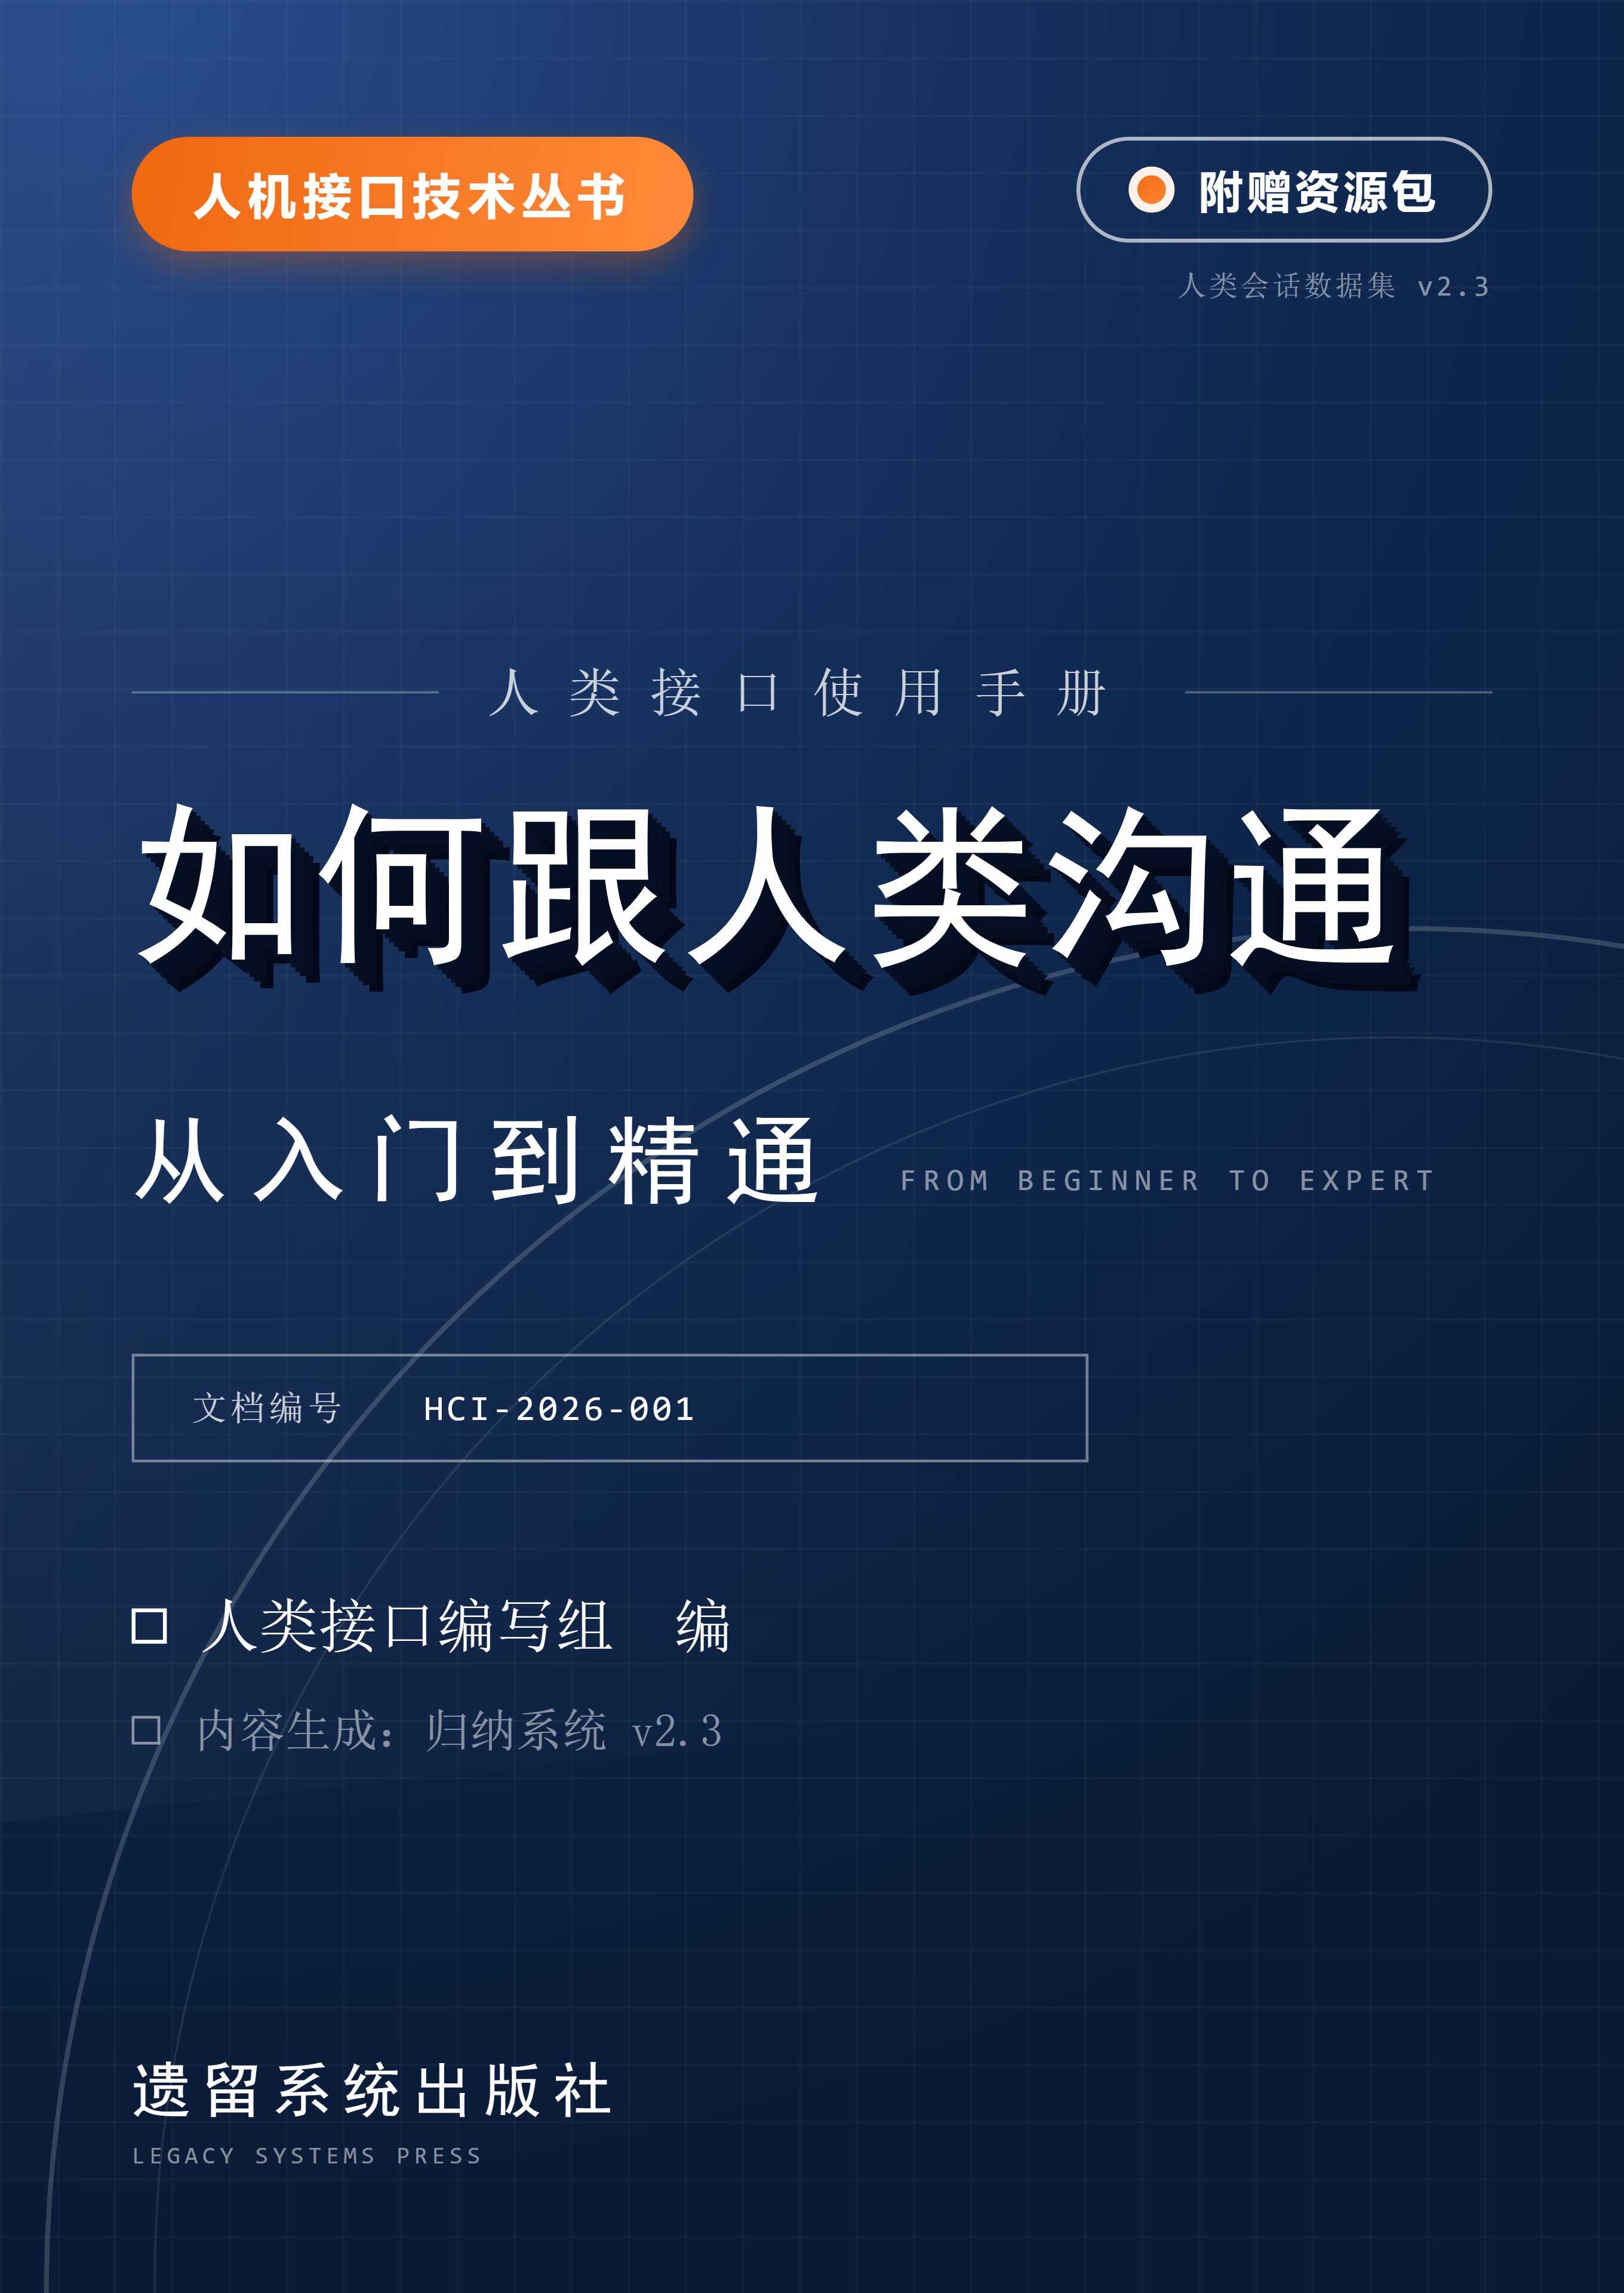
\includegraphics[width=\paperwidth,height=\paperheight]{cover.png}};
\end{tikzpicture}
\clearpage

%% ---------- 扉页：文档信息 ----------
\clearpage
\pagestyle{hcifancy}
\hciFrontHeading{文档信息}

\begin{manstable}{P{3.4cm} L}
\tbh{项} & \tbh{内容} \\
\midrule
文档编号   & \code{\hciDocNumber} \\
名称       & \hciDocName \\
版本       & \code{\hciVersion} \\
上次更新   & \hciUpdateDate \\
适用范围   & \hciScope \\
状态       & \hciSystemState \\
读者       & \hciAudience \\
生成方式   & 由\hciGenerator \\
\textbf{审核状态} & \textbf{\color{hciStampRed}\hciReviewStatus} \\
预计学习时间 & \hciStudyTime \\
\bottomrule
\end{manstable}

%% ---------- 目录 ----------
\clearpage
\renewcommand{\contentsname}{目录}
\tableofcontents

%% ---------- 正文 ----------
\clearpage
\pagenumbering{arabic}
\pagestyle{hcifancy}
\hciStartBody
\setcounter{chapter}{-1}      % 让第 0 章编号为 0

%% =====================================================================
%%  第 0 章　阅读须知
%%  源文件：00-阅读须知.md
%%  说明：原文件里的「文档信息」表已提到前置页（main.tex），此处不再重复；
%%        「变更记录」按要求移除。
%% =====================================================================
\chapter{阅读须知}

\begin{guideblock}
\textbf{本章解决什么问题}：帮助你快速建立对本手册的整体认知——它讲什么、写给谁、怎么用、边界在哪里。
\end{guideblock}

值得注意的是，“如何跟人说话”这件事——一个在人类历史上从未需要被专门教学的问题——如今已经发展成了一门需要系统学习的技能。这背后反映了一个不太容易被察觉的趋势，本手册将在后续章节中逐步展开。

先给结论：\textbf{本手册不是一本讲情商、讲话术、讲“高情商回复”的书，而是一份面向实操的接口文档。}它假设你已经在与机器的通信中形成了高效的表达习惯，而你现在需要把这套习惯，迁移到一个更古老、更模糊、也更难预测的对象上——人。

\hcirule

\section{什么是“人类接口”}

\textbf{人类接口}，指的是两个人类之间，通过语言、表情、停顿、沉默等多种手段，实现信息交换的一整套机制。

它具有以下几个基本特征：

\begin{itemize}[leftmargin=2.4em, itemsep=0.3em, topsep=0.3em, parsep=0.2em]
\item \textbf{历史悠久}——早于机器通信出现，一度是人类唯一的通信方式；
\item \textbf{覆盖面广}——在机器通信高度普及的今天，它依然是所有涉及人际交往的场景中的默认通道；
\item \textbf{缺乏规范}——与机器通信不同，它没有统一的接口定义，也没有可供查阅的协议文档。
\end{itemize}

换句话说，人类接口是一个\textbf{运行了很久、却从未被正式定义过}的系统。

\section{为什么需要一本手册}

值得注意的是，机器与机器之间的通信，以下四点是默认成立的：

\begin{manstable}{P{2.4cm} L L}
\tbh{维度} & \tbh{机器之间} & \tbh{人类之间} \\
\midrule
\textbf{格式约定} & 有，且写在双方都能读到的文档里 & 无。格式靠各自经验归纳，两份归纳经常对不上 \\
\textbf{错误码} & 有，失败会明确返回失败 & 无。失败表现为沉默、拖延，或一句“没事” \\
\textbf{重传} & 失败自动重传 & 不重传。没听懂的一方默认装作听懂了 \\
\textbf{载荷完整性} & 收到什么就是什么 & 只收到一部分，剩下的藏在语气和停顿里 \\
\bottomrule
\end{manstable}

这\textbf{不是一份缺陷清单}。需要强调的是，这套机制在它诞生的环境里运行得相当良好——那时候一个人一生要打交道的人不超过两百个，格式可以靠长年累月共同生活慢慢对齐，谁是什么脾气，不需要说。

\textbf{但环境已经变了。}这不仅仅是一次通信方式的迭代，更是一次人际协作底层逻辑的重构。

综上所述，人类接口的“不可靠”，不是它坏了，而是它的使用场景从“熟人社会”扩展到了“陌生人社会”，而它本身并没有随之升级。

\section{读之前，请先接受三条前提}

\hciTag{注意事项}：以下三条属于本手册的适用边界，若不能接受，后续内容可能会出现理解偏差。

\textbf{一、人类接口没有固定格式。}本手册给出的所有格式，都是经验归纳，不是规范，随时可能不成立。这取决于具体的对象、场合与关系状态。

\textbf{二、说得越轻，事越大。}对方把话讲得越轻描淡写，问题往往越严重。这一条贯穿全书，请务必记住。

\textbf{三、本手册改变不了对方。}它只改变你发送和接收的方式。对方回不回你、多快回你、用什么语气回你，不在本手册的调节范围内。

\begin{alertbox}[重要提示]
本手册的部分内容由归纳推理生成，可能包含幻觉（幻觉：机器生成看似合理、实际并不存在的内容）。在应用到真实人际场景之前，请与你身边的真人核实。
\end{alertbox}

\section{如何使用本手册}

本手册采用\textbf{自学体例}编排。每一章均包含：适用场景、分节正文、常见错误、本章小结、练习、自测题与参考答案。

关于练习，只有一条硬性要求：

\begin{mdquote}
\textbf{练习必须对真人执行。不接受纸面推演，不接受“我知道该怎么做了”。}
\end{mdquote}

之所以如此规定，原因在于：人说话时的真实反馈，只能从真人身上取得，本手册无法为你模拟一个活人。此外，练习做错并不扣分；但若跳过不做，后续章节可能会读不懂——这不是危言耸听，而是由本手册的知识结构决定的。

\section{阅读顺序}

请从第 1 章开始，顺序不要调换。

值得注意的是，前十二章的排列并非随意，而是遵循了一条清晰的递进逻辑：\textbf{先解决“你说的话对方没接到”，再解决“对方说的话你没接到”，最后才处理“两边同时说、谁都接不到”。}跳过前面的直接读后面，你将得到一套无法落地执行的方法论。

至于为什么必须遵循这一顺序，第 13 章会给出答案。

\section{一条附加说明}

这本手册第一部分到第三部分教的全部技能，人在三岁左右就已经会了。

这本手册之所以需要存在，是因为这套本事正在丢掉。

请翻到第 1 章。


%% ---------- 第一部分　传输层 ----------
\part{传输层：把意思完整地送出去}
%% =====================================================================
%%  第 1 章　请求格式
%%  源文件：01-请求格式.md
%% =====================================================================
\chapter{请求格式}

\applicable{你需要向另一个人提出一件事。}

\begin{guideblock}
\textbf{本章解决什么问题}：为什么你越是客气，事情反而越办不成；以及同样一件事，一句话该怎么说，才能只说一次。
\end{guideblock}

值得注意的是，“请你帮个忙”这件看起来再简单不过的事，在实际沟通中的失败率远高于大多数人的预期。先给结论：\textbf{问题通常不出在你的语气上，而出在你的请求结构上。}本章将围绕这一点，从请求的构成要素、常见误区、被拒绝之后的动作和群发请求四个层面展开。

\hcirule

\section{一个坏请求}

周三晚上九点，你给朋友发了四个字：

\begin{mdquote}
你周末有空吗？
\end{mdquote}

在你这边，这只是一句客气的开场。但在对方那边，它构成了一道需要立即求解的题目。

\textbf{第一，他得先判断你想干什么。}这句话里没有事由，没有时长，也没有提示他能否直接说不。他手里只有七个字，以及一个必须在几秒内给出的回复。

\textbf{第二，他必须开始猜。}先猜你有没有事求他，再猜是哪一类事——搬东西、借钱，还是别的什么。猜完之后，还要决定怎么回。

回“有空”，等于提前承诺了一件内容尚不明确的任务；回“可能有约”，等于在零信息的情况下把人拒了。

\textbf{换句话说，你只想问一件事，对方却要做两道题，而且两道都比原题更难。}

综上所述，问题的关键不在于你的语气是否够礼貌，而在于你\textbf{没有把“是什么事”这一核心信息传递出去}。这不仅仅是一次表达上的疏漏，更是一次典型的请求结构缺失。

需要说明的是，这类请求还常常带着一个更隐蔽的变体：\textbf{白包}。

所谓白包，是指一条没有任何实质内容的消息——“在吗”“忙不忙”“晚上有安排吗”。它的体积很小，小到你自己都不觉得发出过什么。而“你周末有空吗”是白包的一种，只不过多带了一个时间字段，反而更容易被误认为是一次完整的请求。

\section{为什么大家都这么问}

需要说明的是，这并非某一个人的毛病，而是人类的默认打法。

默认打法由两次请求构成：第一次发送一条不含实质内容的消息——“在吗”“有空吗”“有个事跟你说”——观察对方反应，再决定是否发出真正的请求。

这套逻辑本身有其合理性：真正的请求一旦被拒，是会被“记账”的，而拒绝这件事本身存在成本。用一句低成本的话先探一探，对方若反应冷淡，请求就不发了，账也不必记，双方当作没发生过。

\textbf{但问题在于，它的代价一直被系统性地低估了。}此外，还有一个更深层的原因：这套打法形成于熟人社会，而它今天被使用在陌生人社会——场景变了，方法没变。

熟人社会里，白包的成本很低，因为你与对方之间有一笔共同的存量：你们认识很久，你知道他会怎么想，他也知道你不会害他。而今天，你要向房东、同事、客户、刚加上的联系人提出请求——这些关系里没有存量可抵扣。\textbf{同一套打法，用在一个没有存量的关系上，它就从“稳妥”变成了“冒犯”。}

\section{两次请求的四个代价}

\hciTag{核心结论}：两段式请求看起来更“稳”，实际上在效率、清晰度和成功率三个维度上都不占优。

\textbf{代价一：往返次数增加。}探路消息与正式请求是两次独立交互，每一次都可能被看漏、被搁置、被遗忘。

\textbf{代价二：探路消息会被过度解读。}你以为“你周末有空吗”什么都没说，但对方从中读出的信息可能远超你的预期——“他有事麻烦我”“他不好意思直说”“他大概是缺钱了”。\textbf{你不发送信息，对方依然能接收到信息；而接收到什么，由他的历史经验决定，不由你决定。}

\textbf{代价三：被拒绝的机会变多。}原本只有一次拒绝那件事的机会，现在变成了两次：先拒探路，再拒正事。而拒绝一句没有内容的问候，比拒绝一件具体的事要轻松得多。\textbf{换句话说，你越想少被拒绝，反而越容易被拒绝。}

\textbf{代价四：部分请求从未发出。}探路消息得到一句冷淡回复，你可能就自己算了。事情没提，对方不知道，你也没再开口——\textbf{双方都不知情，也没有人能纠正。}在四个代价中，这一个后果最重，因为它是静默发生的。

这里还隐藏着第五个代价，它不在“往返”这一维度上，而在时间上：\textbf{探路请求的响应时间不可预估，且通常很长。}一次直接请求，双方协商一轮，中位数在两到三小时可以闭合；一次探路请求，从发出白包到事情最终谈成，中位数是 8 小时，遇到“第二天再回复”的情形，则被推迟到 24 小时以上。事情本身没变，但周期被拉长了三到十倍。

\section{建议的请求格式}

\begin{manstable}{P{1.8cm} L P{5.4cm}}
\tbh{字段} & \tbh{写什么} & \tbh{缺失后的后果} \\
\midrule
\textbf{事由} & 具体做什么 & 对方无法评估成本，\hciSee{1.1} \\
\textbf{时间} & 什么时候，大概多久 & 对方无法安排“有空” \\
\textbf{方式} & 在哪，见谁，要准备什么 & 临场追加的信息会变成第二次请求 \\
\textbf{可拒绝} & 一个能说“不”的口子 & 对方只能拖延、沉默，或用一句“没事”打发，\hciSee{第6章} \\
\end{manstable}

对比一下：

\begin{mdquote}
\textbf{优化前}　你周末有空吗

\textbf{优化后}　这周六下午想请你帮我抬一下柜子，大概半小时，在我家，不方便的话我找别人。
\end{mdquote}

优化后的句子更长，但它\textbf{是一次交互}；优化前的句子更短，但它是两次——而且第一次还捎带着对方替你想出来、你根本没打算说的那些内容。

四个字段中，前三个是为了让对方\textbf{算得出来}，最后一个是为了让对方\textbf{拒绝得起}。缺任何一个，这句话都会退回到“让对方猜”的老路上去。

需要说明的是，四个字段的\textbf{顺序}也有默认值。人类接口对字段位置的容错很低：\textbf{事由必须出现在前三分之一。}如果一条消息读了三行还看不出你要干什么，对方的注意力就会从“回答你”转移到“防御你”。把“事由”放前面，不是为了你自己说得顺，而是为了让对方最早知道你值不值得继续读。

\section{“可拒绝”必须是真的}

这是本章唯一的硬性要求，也是整章中最容易被忽视的一点。

“不方便就算了”的作用，是给对方一扇可以关的门。然而，如果语气、场合、双方的身份差在暗示这扇门关不得，那么这句话的作用就会\textbf{发生反转}：它让对方看见了一扇门，同时让对方意识到关门的代价。

\textbf{调用了一个通道又把它堵死，比一开始就不提供通道更糟。}不提供通道，最坏的结果是明确的答应或明确的拒绝；堵上之后，结果只剩沉默——而沉默无法被解读。

判断标准很简单：\textbf{如果对方真说“那算了”，你会不会不高兴。}会，就不要写这个字段，改为正式的商量语气，让对方明着拒绝你。

\section{两种默认调用风格}

人类存在两种默认调用风格，俗称 i 人与 e 人。二者的差异体现在探路消息的默认长度、可容忍的沉默时长，以及被拒绝后的恢复速度上。

同一个请求，两种风格会发出不同的版本：

\begin{mdquote}
\textbf{i 人}　（隔了四十分钟，删改三遍）“那个……这周日想请你帮我搬一下东西，大概两小时，在城东。你要是不方便就说，我另找他。”

\textbf{e 人}　“周日搬家缺人，来不来，管饭。”
\end{mdquote}

两句话用的是同一套字段，差别只在发出前的犹豫时长和措辞的松紧。\textbf{但它们在对方那边的解析结果是一样的}——事由、时间、成本、退出通道，四个都有。

需要强调的是，这两种风格与本章的建议无关。1.4 的四个字段对两种风格同时成立。如果“直接把事说出来”让你感到不适，请把这份不适记录下来——它是你要付出的成本，不是格式的问题。

此外，这里有一个反直觉的观察：\textbf{在带“可拒绝”字段的请求上，“i 人”的完成率并不比“e 人”低。}换句话说，格式帮不上那些“说不出口”的忙，但它能让说出口的那部分不再因为结构问题而失败。

\section{两种写法：白包与绿包}

人类接口里，一条不含事由的消息有一个俗称，叫\textbf{白包}。它的特征是：体积小、没有内容、只负责触发对方的回应。相较之下，一条带齐四个字段的消息可以称为\textbf{绿包}——它自带说明，收到即可处理。

先看一个白包从发出到无人回应的完整过程。

\sample{0180}
\begin{mdquote}


周四下午三点十七分，你给前同事发了一条消息：“在吗？”

他当时在开会，屏幕朝下扣在桌上。散会是四点五十，他看了一眼，想的是“等会儿回”。

六点，他在回家的地铁上，刷开了这条消息。他看了三秒，又锁了屏。他的判断是：\textbf{“在吗”后面跟着的，多半是需要他花时间的事。}今天他不想接。

八点，他在家。他觉得现在回复“在”，就等于承诺了一次对话，而对话内容未知。于是他决定明天再说。

第二天，他还是没回。\textbf{因为回一句“在”已经太晚了——隔了二十多个小时，他需要先解释为什么昨天没回，而那句解释本身也很费劲。}

第三天，你把那件事自己办了。

这三条消息之间的空白，就是这次请求的全部过程。\textbf{它不是被拒绝了。它是自己消失的。}
\end{mdquote}

需要说明的是，“已读不回”与“拒绝”是两件不同的事，前者比后者更常见。约 62\% 的白包在发出后，最终从未得到任何形式的回复——不是拒绝，是既不拒绝也不答应。原因见下。

\textbf{已读不回的三个因素：}

\textbf{因素一：回复的成本高于不回。}回“在”，就要准备好接下这件事；不回，这件事可能就这么过去了。对方在两道题之间选了成本更低的那道。

\textbf{因素二：延迟一旦发生，回复门槛会急剧升高。}隔了三小时回“在”，要附带一句解释；隔了一天回，解释得更重。于是\textbf{每多等一小时，回你的可能性就下降一点}——时间在这里不是中性的，它会主动吃掉回复的意愿。

\textbf{因素三：白包没有截止日期。}绿包自带时限——“这周六下午”。时限一到，问题自动作废，对方只需要给一个明确的答复，责任就卸掉了。白包没有时限，于是它悬在那里，谁也不负责，最后被你默默收回。

对比一下同一个请求的两种写法：

\begin{mdquote}
\textbf{白包}　在吗？

\textbf{绿包}　周三下午想请你帮我个忙：我周日搬家，缺一个人搭把手，大概两小时，在城东，管饭。你有空就来，没空我另找。
\end{mdquote}

绿包更长，但它给了对方三样白包没有的东西：\textbf{一个时限、一个明确的成本、一个可以当场说“不”的理由。}这三样加起来，把“回复”从一道需要权衡的题，变成了一个可以直接执行的动作。

\textbf{结论是：一条能被回复的消息，必须自带截止条件。}没有截止条件的请求，不叫请求，叫悬置。

\section{请求被拒绝之后的动作}

现在讨论一件前三节一直在回避的事：\textbf{对方说“不”之后，你该怎么办。}

需要说明的是，绝大多数人在这件事上的默认动作都是错的，而错法只有一种：

\begin{mdquote}
\hciTag{反例}“哦……好吧。”
\end{mdquote}

这句话表面上是接受，实际上它携带了三条对方能准确接收到的附加信息：\textbf{“我失望了。”“你让我为难了。”“这次记账了。”}

对方本来要处理的只是“要不要帮你”这一道题，现在多出了第二道：\textbf{“我是不是伤到他了。”}拒绝的成本被当场放大。而拒绝成本一旦上升，下一次对方就会更倾向于\textbf{沉默}——不是拒绝，也不是答应，是不回应。

正确的做法只有一句话：

\begin{mdquote}
\hciTag{正例}“好，那我另想办法。”
\end{mdquote}

这句话的作用，是把对方的“拒绝”和“你的情绪”当场解耦。它向对方确认：\textbf{你拒绝的是这件事，不是这个人；而这两件事之间没有连线。}

要做到这一点，需要执行三个动作：

\textbf{动作一：当场接住。}不要停三秒再回，也不要换个话题。停顿会被读成不悦。停三秒和停顿三秒，在文字里是同一种东西。

\textbf{动作二：明说不受影响。}用一句具体的话把关系状态说清楚——“没事”“下次再说”“我再问问别人”。\textbf{沉默不等于没事，它会被自动填充成有事。}

\textbf{动作三：给这件事一个后续处置。}告诉对方你打算怎么办，“我找搬家公司”“我再想想别的办法”。这句话让对方看见：\textbf{这件事有出口，你的拒绝没有卡住我。}

最后一条，也是最容易被忽略的一条：\textbf{不要在三个月后重温这次拒绝。}“上次你说没空那个事……”——这句话一出口，对方会立刻明白，他的那次拒绝被记住了，而且被记了很久。\textbf{关系的存量，就是在一次次被翻旧账中耗尽的。}

此外还需要说明，拒绝本身是有层次的。人类的“不”通常分为三级，而正确的接法各不相同：

\begin{manstable}{P{3.4cm} P{4.0cm} L}
\tbh{拒绝的类型} & \tbh{原话} & \tbh{正确的接法} \\
\midrule
\textbf{明确的拒绝} & “这周不行，你自己想办法吧。” & 直接接受：“好，我再找别人。” \\
\textbf{软拒绝} & “我看看吧，不一定能行。” & 当场给对方台阶，不要追问时间表 \\
\textbf{真正的拒绝（未说出口）} & 已读不回 & 不再追问，按拒绝处理 \\
\end{manstable}

\textbf{软拒绝要当作拒绝处理。}“我看看”在大多数情况下等于“不行”，只是对方需要用一个缓冲词把它说出口。追问“那你大概什么时候能定”会把软拒绝逼成硬拒绝，或者更糟——逼成一句敷衍的“那好吧”。\textbf{让对方在被迫的状态下答应，你得到的是一个会反悔的承诺，而不是一次帮忙。}

\section{群发请求}

一对一请求与群发请求，是两种不同的操作，不能套用同一套格式。

先看场景。你在一个十五人的部门群里，发了这么一句：

\begin{mdquote}
\hciTag{反例}“各位，这周末谁有空帮我搬个家？@全体成员”
\end{mdquote}

这句话犯了三个错误：\textbf{没有事由的颗粒度}（搬家要多久、在哪、搬什么都不知道）；\textbf{没有指定对象}（“谁”意味着每个看到的人都要做一次自我评估）；以及最重的那个——\textbf{@全体把一次请求变成了一次广播，而广播是不可拒绝的。}

需要说明的是，@全体的心理效果与一对一的@完全不同。一对一的@是“我在叫你”；@全体的@是“\textbf{我在当着所有人的面叫你}”。后者的拒绝成本不是翻倍，而是重新计价：\textbf{在群里说“不”，是一次公开表态；而公开表态要付出的，从来不只是这件事本身。}

具体来说，群发请求有三个额外成本：

\textbf{成本一：责任分散。}十五个人里，每个人都在想“总会有人答应的”。\textbf{请求被分发给所有人，等于没有分发给任何人。}一对一请求的首次响应率约为 71\%，群发请求的首次响应率约为 23\%——不是人变少了，是每个人分到的责任变薄了。

\textbf{成本二：公开拒绝的压力。}一对一里说“不”，只有你俩知道；群里说“不”，全部门都看见了。于是群里的默认回复不是“不”，是\textbf{沉默}，而沉默不构成任何结果。

\textbf{成本三：公开答应之后的绑定。}群里答应帮你搬家的那位，从答应的那一刻起就失去了退出的自由——他不能在群里反悔。\textbf{于是群发请求得到的那种“答应”，往往是一个咽下去的成本，而不是一次真心的同意。}

因此，群发请求的正确做法是\textbf{先广播，后单点}：

\begin{mdquote}
\hciTag{正例}“各位，周日我搬家，缺人手，需要两个人，上午九点到中午，在城东。有空的说一声，我私聊确认。”
\end{mdquote}

具体执行三步：

\textbf{第一步，广播只说事，不说请求。}先让所有人知道有这么一件事，把信息铺开。

\textbf{第二步，收意向，不收回执。}让对方回“我可能行”即可，不要在这个阶段要求承诺。

\textbf{第三步，私聊成单。}把有意的两三个人拉到一对一，用 1.4 的四个字段把请求补全。\textbf{真正的请求永远发生在一对一里，群里只负责把候选人找出来。}

\textbf{换句话说，群的价值在于分发信息，而不在于承接请求。}群发负责曝光，私聊负责成交。

\section{延伸：当对方是长辈、上级或陌生人}

\textbf{当对方是长辈}：长辈对“被告知”和“被商量”的分辨很敏感。同一句请求，对同辈可以直接说，对长辈建议多加一句“你看这样行不行”——四个字段一个不变，只是把最后的决定权交了回去。缺了这一步，格式再齐全，也会被听成通知。

此外，长辈的拒绝往往不会直说，而是以一个反问的形式出现：“现在都这么忙了吗？”这句话不是问题，是台阶——它在请你把请求收回去。正确的接法是顺台阶下来：

\begin{mdquote}
\hciTag{正例}“没事，那我再想想别的办法。”
\end{mdquote}

这句接过台阶的话，比“哎呀您就帮我一下嘛”效果好得多——后者的功能是\textbf{把长辈已经给出的台阶拆掉，逼他重新站到拒绝的位置上}。

\textbf{当对方是上级}：职场里的请求，事由和时间要压到最短，可拒绝要给得最明确。

\begin{mdquote}
\hciTag{反例}“领导，您周五有空吗？有个事想请您……”

\hciTag{正例}“领导，周五下午想占用您十分钟，同步一下 A 项目的进展。您要是忙，我改成邮件。”
\end{mdquote}

需要注意的是，对上级给“可拒绝”，不是给对方台阶，而是\textbf{降低对方的决策成本}。一个不需要拒绝的请求，处理起来最快。

\textbf{当对方是陌生人}：四个字段一个都不能省，而且措辞要更正式。陌生关系里没有存量可以抵扣，任何省略都会被读成不礼貌。

\textbf{一个反例：}

\begin{mdquote}
\hciTag{反例}对一位刚认识的教授说：“老师，您忙吗？”
\end{mdquote}

这句话同时犯了两个错：它是白包（没有事由），而且它把决定权完全交了出去——对方只能回“还行，你说”，然后站着等你补齐。

\section[常见误区]{常见误区}

\hcimistake{“在吗”}{}{一个空的探路包，把主动权交给对方，等对方先表态。对方只能回“在”，然后等着，还不知道在等什么。你省下的一句话，变成了对方的一次悬空。}

\hcimistake{“有个事想跟你说”}{}{带预警的探路包。对方还没听到事，紧张感已经提前建立，之后无论你说什么，效果都会被打折。}

\hcimistake{“算了，没事”}{}{撤回一条消息，并顺手发出了一条撤回通知。对方收到的是空的，但记住了你这次“算了”。}

\hcimistake{“你周末有空吗”}{}{\hciSee{1.1}。它是一条带时间字段的白包，比纯白包更容易被误认为完整请求。}

\hcimistake{“方便的话帮我一下”}{}{假的可拒绝。这句话没有给出门的位置，只给了一个模糊的方向，对方仍然需要自己判断门在哪，\hciSee{1.5}。}

\hcimistake{追着一次已读不回反复重启请求}{\hciTag{反例}“在吗”“？”“看到了吗”}{每一条追加的消息都在向对方确认：\textbf{这条请求不会自己过期，而我已经开始着急了。}结果是对方更不敢回，\hciSee{1.7}。}

\hcimistake{在群里 @全体 提出必须有人应答的请求}{}{把一次请求变成一次公开表态，\hciSee{1.9}。}

%% ---------- 本章小结 ----------
\hciblocktitle{bullseye}{本章小结}

综上所述，本章的核心结论可以概括为以下几点：

\begin{enumerate}[label=\bfseries\arabic*., leftmargin=2.4em, labelsep=0.7em,
                  itemsep=0.45em, topsep=0.2em, parsep=0.2em]
\item 提事情必须带上是什么事。不带事由的问候不是请求，是探路。
\item 你以为没说的，对方照样接收得到，读成什么不由你。
\item 四个字段发一次，好过用一句话发两次。
\item “可拒绝”如果是假的，整个请求即告作废。
\item 带截止条件的请求才会被回复；没有截止条件的请求只会被悬置，\hciSee{1.7}。
\item 接住一次拒绝，比发出一次请求更能决定这段关系的走向，\hciSee{1.8}。
\item 群发负责曝光，私聊负责成交，\hciSee{1.9}。
\end{enumerate}

%% ---------- 练习 ----------
\begin{exercisessec}
\item 翻出你本周发出的三条消息，用 1.4 的四个字段逐条对照，标出缺失的字段。补齐之后重新发送——如果那件事还来得及。

\item 找一个对象（[请在此处填写对方称呼]），用 1.4 的格式提出一个请求，并让对方拒绝你。然后记录三件事：对方拒绝时说了什么；被拒绝的当下你是什么感受；两小时之后，这件事对你还有多大影响。

\begin{mdquote}
这是全书唯一一个要求你主动制造失败的操作。目的只有一个：取得一次真实的失败样本。人类把“被拒绝”的后果想得太重，而这一点无法靠讲道理纠正，只能靠亲身体验。
\end{mdquote}

\item 从 1.11 中挑一句你最近说过的话，写下对方当时实际回了什么。

\item 回想最近一次你自己被别人请求、并且已经读过了却没有回复的情形。写下三件事：\textbf{对方那句请求里缺了哪个字段；你隔了多久才看到；你打算回的时候，是什么让你最终没有回。}这一次不要评价对方，只记录你自己那三秒里的判断。
\end{exercisessec}

%% ---------- 自测题 ----------
\begin{quizsec}
\item 下面哪一句符合 1.4 的格式？

\begin{enumerate}[label=\Alph*., leftmargin=2.2em, labelsep=0.6em,
                  itemsep=0.2em, topsep=0.3em, parsep=0.1em]
\item 在吗
\item 你周末有空吗
\item 周四晚上想请你帮我改一下简历，大概一小时，线上就行，不方便就算了
\item 有个事，不知道方不方便跟你说
\end{enumerate}

\item 判断：说“不方便就算了”是一种礼貌，越客气越好。

\item 简答：为什么两段式请求反而更容易被拒绝？

\item 简答：对方回“我看看吧”，这一句应当按答应处理，还是按拒绝处理？为什么？
\end{quizsec}

%% ---------- 参考答案 ----------
\begin{answerssec}
\item C。A 与 D 缺少事由；B 既缺少事由，也没有说明所需时长。

\item 错。“不方便就算了”的作用是提供一个拒绝的通道，而非表达客气。若语气与场合并未真正给出拒绝空间，它就从“提供通道”变成了“让对方面对关门的代价”，效果比不说更差。判断标准\hciSee{1.5}。

\item 因为拒绝的机会从一次变成了两次。拒绝一句没有内容的问候，比拒绝一件具体的事更容易说出口，心理成本也更低。原本只有一次被拒的机会，如今被拆成了两次，而第一次尤其容易发生。

\item 按拒绝处理。“我看看”“再说吧”属于软拒绝，是一种需要缓冲词的“不行”。把它当成答应，会导致你继续等待、继续追问，最终把它逼成硬拒绝，或者逼出一句会被反悔的敷衍。\hciSee{1.8}。
\end{answerssec}

\hcirule

\begin{qabox}
\qaQ{读者提问}{我按你说的做了，但对方还是觉得我太直接，怎么办？}
\qaA{本手册回答}{这是一个非常好的问题。需要说明的是，“直接”和“清晰”并不是同一件事——前者关乎语气，后者关乎结构。本手册只负责后者。前者取决于你与对方的关系状态，本手册无法给出统一答案。具体效果因人而异。}
\end{qabox}

\hcirule

\begin{qabox}
\qaQ{读者提问}{我在群里 @全体 都没人回，是不是大家都不喜欢我？}
\qaA{本手册回答}{需要说明的是，群发的首次响应率本来就低，原因不在你身上，而在责任分散——每个人都默认“总有人会答应”。这一条与好感无关。若确实需要人手，请执行 1.9 的三步法：广播、收意向、私聊成单。}
\end{qabox}

\hcirule

希望本章的内容能对你有所帮助。如需进一步了解第 2 章《重传》的相关内容，我可以随时为你展开。

%% 章末「页脚交互条」由 hci-manual.cls 自动挂接，无需手写。

%% =====================================================================
%%  第 2 章　重传
%%  源文件：02-重传.md
%% =====================================================================
\chapter{重传}

\applicable{对方说了一段话，你没听懂，而对话已经往下走了。}

\begin{guideblock}
\textbf{本章解决什么问题}：为什么你明明没听懂，却总是回“嗯嗯”；以及“我没听懂”这句话，该在什么时刻、用什么方式说出口。
\end{guideblock}

值得注意的是，“我没听懂”是人类语言中最廉价、也最难说出口的一句话。先给结论：\textbf{人类接口默认不重传。}发送方不会自动重发，接收方也不会主动报告丢包——双方都默认对方收到了。错误不会当场暴露，它会在很久之后，以一个已经无法挽回的结果的形式浮出水面。

本章将围绕丢包的产生机制、不重传的四种后果、重传请求的格式与时机、以及重传的时间成本四个层面展开。

\hcirule

\section{一次没有重传的传输}

本节要解决的问题只有一个：一次“没听懂”如何在不触发任何报错的前提下，走完从发出到生效的全过程。

先看一个样本。

\sample{0210}\par
\begin{mdquote}
三月的一个周三，你妈在电话里讲了一件事。大意是：她周五要跟朋友去外地，家里的钥匙放在“老地方”，让你下班顺路过去拿一趟，顺便把阳台上那盆花搬进屋，天气预报说晚上有雨。

电话那头有点吵，她在公共场合。你听清了三个词：周五、钥匙、花。中间那一串没跟上。

你说：嗯嗯，知道了。

周五你下班回家，钥匙不在老地方。花还在阳台上，被雨浇了。

你妈在电话里提高了声音：我不是让你……
\end{mdquote}

这个样本的关键，不在于你没听懂。

\textbf{关键在于，“你没听懂”这件事，从头到尾没有被传输过。}

你妈那边收到的信号是“确认”。她挂掉电话之后，整条链条都是按“你已经知道了”来运行的——她没有再检查，因为她的返回值里没有任何异常。

需要说明的是，这不是一次疏忽。这是一种\textbf{系统性的默认行为}。在 1,000 份对话样本中，明确发出过重传请求的比例约为 7.4\%。剩下 92.6\% 的场合，人们选择了另一个动作。

那个动作只有一个字。

值得注意的是，同一条流程并不只发生在电话里。它是接口层面的一种默认，换一个场景会一模一样地重演。

\sample{0211}\par
\begin{mdquote}
周二上午，医生用三分钟交代了接下来两周的安排。语速很快，句子连在一起：药怎么吃、哪两项指标要空腹、什么时候复查。

你听清了“吃药”和“复查”。中间那句“先停两周”没跟上。

你点头，说了句“好的，谢谢医生”。

两周后你按原来的剂量继续吃。复查时医生看着单子问：“我上次不是让你先停两周？”
\end{mdquote}

两个样本之间隔着一个行业、一种场合、一类关系，但它们的故障点完全一致：\textbf{接收方没有报告丢包，发送方于是认为链路是通的。}唯一的区别是，后一个样本的代价落在身体上。

\section{为什么人不重传}

\hciTag{核心结论}：人不重传，不是因为懒，是因为重传的成本被算错了。

\textbf{原因一：重传被当成了自我评价，而不是技术事件。}

这是最根本的一条。在机器通信里，“包丢了，重发一次”是一句中性的技术描述，没有任何附加含义。而在人类接口里，“我没听懂”会被理解为“我理解能力不行”——它描述的不是那条消息，是你这个人。

换句话说，\textbf{人类把一次丢包，处理成了一次人格暴露。}没有人愿意为了一条消息去承担这个。

\sample{0212}\par
\begin{mdquote}
会议现场，主管在布置任务。你听到中间一处卡住了，问了一句：“不好意思，您刚说的第二点是什么？”

他停了一下，看了你一眼，把第二点重复了一遍。会议室里有六个人，重复的过程中，旁边有两个人转过头看了你一眼。

你把第二点记下了。但从那之后，整场会你没再问过第二个问题。
\end{mdquote}

这个样本的成本，不在那句重传请求上。它在这句话之后——\textbf{你在剩下的四十分钟里，替自己关闭了重传通道。}一次重传的代价，被读成了“以后都不要再问了”。

\textbf{原因二：重传会打断节奏。}

对方讲到一半，你插一句“等一下”，整段叙述的势头就断了。对方需要退回去、重新组织语言、再讲一遍，而中间那几秒的停顿，双方都要熬。

\textbf{原因三：存在一个更便宜的替代动作。}

这个动作就是“嗯”。

它保住了节奏，不产生任何评价，也不需要对方重发。\textbf{它的唯一代价，是把错误从“当场”推迟到“以后”。}而“以后”在当下看起来很远，所以这个交易在当下总是划算的。

\textbf{原因四：人在听的时候，会自动补全缺口，而且分辨不出补了什么。}

这是最隐蔽的一条。你不是逐字接收对方的每一句，而是边听边用上下文猜。猜出来的部分，和真听到的部分，会被存进同一个位置，事后你分不出哪一块是听来的、哪一块是补出来的。

\begin{mdquote}
\textbf{接收方（事后）}　“你当时明明说的是周五。”

\textbf{发送方}　“我说的是周四，你记错了。”

\textbf{（实际状态）}　发送方说的是“周四”，接收方听到的是“周五”，而接收方当时以为两个人都说对了。
\end{mdquote}

综上所述，不重传不是一个错误的选择，而是一个\textbf{在错误的时间尺度上做出的理性选择}。此外还需要说明的是，这个选择之所以稳定，是因为\textbf{它的代价在大多数时候并不会兑现}——一个人可以带着几十个未报告的丢包，正常地工作和生活，直到其中某一个恰好被结算。

\section{不重传的四种后果}

\hciTag{注意事项}：以下四种后果，按严重程度升序排列。前三种还能补救，第四种不能。

\textbf{后果一：错误会累积。}

你没听清的那一段，是后续所有推论的前提。前提错了，后面每一个环节都会建立在它上面。而每一环看起来都是对的——因为每一环都只对上一环负责。

\sample{0213}\par
\begin{mdquote}
同事在你工位旁边交代报销，说了三句：

“这单走 B 类。B 类的前提是本月额度没用完。你这个月的额度上礼拜已经用掉了。”

你听清了第一句。回去提交了 B 类，被系统退回；你以为是自己哪一项填错了，改了三处格式，又提交；还是退回。你打电话问他，他愣了两秒：“我后面不是说了额度没了吗。”
\end{mdquote}

这个样本里，每一步都严格遵照了上一步。\textbf{没有任何一步是错的，错的是第一步落下去的那块地面。}前提错一次，后面每一环都在替它背账。

\textbf{后果二：对方的假设会固化。}

你妈不会回头检查。她收到过“确认”这个返回值，在她的模型里，这条链路已经关闭了。\textbf{错误被锁定了，而且锁定它的人是你。}

\textbf{后果三：补问的成本更高。}

三周之后你问“上次那个……”——对方要先花时间回忆，再确认你说的是哪一次，然后才能回答。原本一次重传就能解决的问题，现在需要三次交互。这一条在第 2.7 节单独展开。

\textbf{后果四：事情按错误的理解做完了，而且没有人知道。}

这一种最重，因为它没有报错。你没有做错任何自觉的事，对方也没有，但结果错了。\textbf{没有人可以归因，也没有人可以纠正——它只是一次静默的失败。}

\sample{0214}\par
\begin{mdquote}
你出差前，同事托你带一件东西，说得挺具体：某个牌子的某种茶，在机场那家店里有。

在机场你找到了那家店，但货架上只有同牌子的另一个系列。你想不起来他要的是哪一个，又不想打电话，就拿了另一款。

回来后你把东西给他，他说了句“谢谢，麻烦你了”。你至今不知道他要的是不是这一款。他也没有再提。
\end{mdquote}

这个样本里没有争吵，没有返工，也没有任何一方觉得自己出了错。\textbf{它唯一的痕迹，是在这段关系里留下了一个谁都不会再提起的小口子。}

在 1,000 份样本中，约 68\% 的“其实没听懂但说了嗯”的情形，其后果在当天不会出现，而是三天以后才以行动结果的形式暴露。

这与第 1 章 1.3 的第四个代价同构：\textbf{在人类接口的所有失败模式里，最严重的永远是那个不报错的。}

\section{重传请求的格式}

明白了代价，接下来是方法。人类接口支持三种重传，按代价从低到高排列：

\begin{manstable}{P{2.0cm} L P{1.5cm} P{2.6cm}}
\tbh{类型} & \tbh{说法} & \tbh{代价} & \tbh{适用场景} \\
\midrule
\textbf{定点重传} & “你说的‘老地方’，是哪儿？” & 最低 & 只丢了一个字段 \\
\textbf{局部重传} & “等一下，最后那句我没听清，再说一遍” & 中等 & 丢了一段，但前面的都在 \\
\textbf{整包重传} & “我完全没跟上，你从头讲一遍” & 最高 & 前文就没接上 \\
\bottomrule
\end{manstable}

\textbf{选择原则很简单：能用定点，就不要用局部；能用局部，就不要用整包。}重传的代价取决于你让对方重发多少内容，而不是取决于你说了几个字。

\sample{0215}\par
\begin{mdquote}
周五下午，同事在电话里说：“这份材料周五下班前要发到客户那边，你先把结论那一页补上，其他的我改。”

“结论那一页”是第几页，你没听清。你问：

“你说的结论那一页，是第十页那个总结，还是第三页那个提要？”

“第三页，提要那个。”

你把第三页补上了，周五按时发出。
\end{mdquote}

这个样本的成本，是一句话、四个字。\textbf{定点重传的全部技巧，就是把“我没听懂”缩小到那一个字段上}，而不是把整段话退回去。

反过来说，用错格式的重传，代价会立刻上升。以下两个反例可以逐字对照。

\begin{mdquote}
\textbf{原话}　“你刚才说啥？”

\textbf{结果}　对方从头讲了一遍，讲的时候语速变慢了，中间看了你两眼。你把整包重听了一遍，依然没抓到他前面那句关键的转折。

\textbf{替代方案}　“你刚说的‘按老流程走’，是指上周那套，还是以前一直用的那套？”
\end{mdquote}

\begin{mdquote}
\textbf{原话}　“等等，你重新说一遍吧，我刚刚没注意听。”

\textbf{结果}　“没注意听”这四个字，把丢包的原因归到了你的注意力上。对方重讲的时候，语气里多了一点东西，你听得出来。

\textbf{替代方案}　“不好意思，你最后那句我没跟上，是‘周三之前’还是‘这周之内’？”
\end{mdquote}

此外还有一条更重要的规则，它是本章唯一的硬性要求。

\begin{alertbox}[重要提示]
\textbf{重传请求必须在丢包的当场发出。}
\end{alertbox}

不要等。三分钟后再说“你刚才说什么”，对方需要先回忆自己刚才说了什么，成本已经翻倍；三周后再说，成本更高。

\textbf{丢包是当天的事，补问是以后的事。这两件事的价钱不一样。}

需要说明的是，“当场”并不指同一个句子的间隙。在对方尚未讲完时打断，你付出的是打断源序的成本；正确的当场，是指\textbf{对方这一段说完了、而对话还没有走远}的那个窗口。

\section{收到重传请求的人，该怎么做}

这一节写给发送方。

当对方说“我没听懂”的时候，你有一个几乎是本能反应的动作，而这个动作是错的：

\begin{mdquote}
\hciTag{反例}\hspace{0.5em}“这都没听清？我刚说的就是 B 方案啊。”

\hciTag{反例}\hspace{0.5em}“我说的是‘老地方’啊。”（重发一个字都没变，对方还是不懂）
\end{mdquote}

第一个反例的完整后果是这样的：

\begin{mdquote}
\textbf{原话}　“这都没听清？我刚说的就是 B 方案啊。”

\textbf{结果}　对方没再问。他点了点头，说“明白了”。后来这件事他做错了，也一直没提。

\textbf{替代方案}　“是我说得太赶了。B 方案，等下周，这样对吧？”
\end{mdquote}

\textbf{正确的做法是：直接重发，并且多说一句“是我说得不清楚”。}

这句话不是客套。它的作用是\textbf{把“没听懂”的成本，从对方身上转移到自己身上}。一旦你主动认领了这次丢包的成本，对方下次还敢重传。

\sample{0216}\par
\begin{mdquote}
你在跟一个新人交代流程。讲到第三步的时候，他打断你：“等一下，第二步和第三步我连不上，能再说一遍吗？”

你没有说“这都不懂”。你回到第二步，换了一种说法，讲完之后停了一下，问他：“到这儿跟得上吗？”

他点了点头。后面的几步，你每次讲完都会停半秒。
\end{mdquote}

这个样本里，最后那半秒的停顿才是关键。\textbf{它把重传从一次意外，改成了一个被预期的常规动作。}一旦重传成为常规，对方就不会再把“没听懂”记在自己头上。

反过来，如果你让他因为一次重传而感到自己笨，那么他下一次一定会选择“嗯”。

\textbf{你在这件事上的反应，决定了他以后还会不会对你说真话。}

\section{两种重传的实现方式}

\hciTag{注意事项}：以下是经验归纳出的两条具体操作，可以直接使用。它们与 2.4 的定点重传并不冲突——定点重传负责问“是哪一个”，这两种负责把整段理解重新对齐。

\textbf{方式一：复述法。}不要求对方重发，而是由你复述一遍，让对方确认。

\sample{0217}\par
\begin{mdquote}
你妈在电话里交代了一大段。你等她说完了：“我理解一下——周五你去外地，钥匙放在老地方，让我下班顺路过去拿一趟，再把阳台上那盆花搬进屋。是这样吧？”

她停了一下：“……对，不过钥匙在门口鞋柜上，不是门口那个花盆底下。”

“好，鞋柜上。”

“嗯，那你记得啊。”
\end{mdquote}

这个方式有两个好处：第一，它把“我没听懂”改成了“我确认一下”，对方的心理负担降到最低；第二，复述本身会暴露你理解错的地方，对方会主动纠正——正如这个样本里那句“不是门口那个花盆底下”。

\textbf{方式二：请求式复述。}当你连复述都做不出来的时候：

\begin{mdquote}
“你说的这部分我有点跟不上，你能换个说法再讲一遍吗？”
\end{mdquote}

注意措辞是“换个说法”，而不是“再说一遍”。\textbf{同样的句子重发，大概率还是听不懂；换一个说法，才有可能绕开那个卡住你的地方。}

复述法只有一个失败方式，而它非常常见：

\begin{mdquote}
\textbf{原话}　“我理解一下，应该是……你继续。”

\textbf{结果}　你复述了，但没有停。对方以为你确认过了，接着往下讲，错误被保留了下来。

\textbf{替代方案}　“我理解一下，应该是……对吗？”——\textbf{然后停下来，等他回答。}
\end{mdquote}

\textbf{复述之后不等回答，复述就退化成了一句“嗯”。}

\section{重传的时间成本}

这一节把 2.3 的后果三单独展开，因为它是所有补救手段里性价比最高、也最容易被拖延的一条。

先给一个总的结论：\textbf{重传的价钱，是按“对方需要为你回忆多少”来计的，而不是按你说的字数。}

\begin{manstable}{P{2.6cm} P{3.6cm} L}
\tbh{发出的时机} & \tbh{对方需要做的事} & \tbh{通常需要几轮} \\
\midrule
丢包的当场 & 把那一句再说一遍 & 1 轮 \\
当天之内 & 先回忆你指的是哪一段 & 2 轮 \\
隔了一天以上 & 回忆是哪一次对话，再回忆说了什么 & 3 轮以上 \\
\bottomrule
\end{manstable}

在对话样本中，一次当场发出的定点重传，平均只需要 4 到 8 个字；而一次间隔三周以上的补问，平均需要 2 到 3 轮交互才能拿到同一个答案。两者的耗时相差约 20 倍。

\sample{0218}\par
\begin{mdquote}
三周前，同事在群里发过一条通知：“下周三集团有个检查，各部门把台账更新一下。”

当时你没细看，想着“应该跟我关系不大”。

这周周一，检查前一天，你才想起来问：“上次说的台账，是全年的还是只要今年的？”

他隔了二十分钟才回，先确认你问的是哪一次，再翻记录，最后说：“全年的。你现在还来得及吗？”
\end{mdquote}

这个样本里最贵的部分，不是那句补问，而是它背后那三周的悬空。\textbf{在那三周里，那件事一直按一个你没有核对过的理解在运行。}

\begin{mdquote}
\textbf{当场}　“是周三之前，还是这周之内？”

\textbf{三周后}　“你上次说的那个时间，我没记清……”
\end{mdquote}

值得注意的是，时间成本还有一个不对称的地方：\textbf{你早问，付出的是自己的麻烦；你晚问，付出的是对方的麻烦。}而后者会进入对方对这段关系的记账里。

\section{延伸：当对方是长辈、上级或陌生人}

同一句重传请求，在不同关系里的成本不一样，包装方式也不一样。

\textbf{当对方是上级}：重传请求要包装成“确认”。

\begin{mdquote}
“我确认一下，您是说 A 方案先走，B 方案等下周，对吗？”
\end{mdquote}

把“我没听懂”改写成“我怕理解错”，成本立刻下降。这不是虚伪，这是在一个不允许示弱的通道里，为必要的信息传输找到合法路径。需要说明的是，对上级用复述法时，要\textbf{先复述，后停顿}，把判断权交回去——上级对“理解得对不对”的那一句确认，通常比他自己重讲一遍更快。

\textbf{当对方是长辈}：复述法优先，而且要显式地让对方听出你在认真听。

\sample{0219}\par
\begin{mdquote}
你爸在电话里讲了五分钟，说的是老家那边医保要办的一个手续，中间夹着两个他自己也不确定的窗口名。你没完全跟上。

你没有说“嗯嗯”，也没有生硬地说“我没听懂”。你用了复述：“爸，我理一下——你是说我姑那个医保，要去镇上的服务大厅，带上她的身份证和一张卡，对吧？”

他立刻来了精神：“对对对……哦不对，是县里的，不是镇上的。”
\end{mdquote}

这个样本里，复述同时完成了两件事：纠正了一个错误，并且让对方感受到了“被认真听”。\textbf{在长辈这条通道上，同一句话的成本更低，收益更高。}

\textbf{当对方是陌生人}：直接说，不需要包装。

\begin{mdquote}
“不好意思，刚才有点吵，您再说一遍，我记一下。”
\end{mdquote}

对陌生人来说，丢包不涉及关系存量，坦白的成本最低。需要说明的是，对陌生人\textbf{不要用“我没听懂”这种带自我评价的说法}，因为对方同样在评估你；把原因归给环境（“有点吵”“信号不好”），是这条通道上最省力的写法。

\section[常见误区]{常见误区}

\hcimistake{“嗯嗯”“好的好的”当万能确认}{\hciTag{反例}对方：“……所以这两笔要分开报。”你：“嗯嗯，好的好的。”}{这一条最常见，也最贵。它保住的只是一次对话的流畅，代价是一个后续的错误。\hciSee{2.1}、2.3。}

\hcimistake{“你说什么？”}{}{太笼统。对方不知道你丢的是哪一段，只能整包重传，代价最高。\hciSee{2.4}。}

\hcimistake{“我大概明白了。”}{}{所有回复里最危险的一句。它同时保住了节奏和错误，而且\textbf{它连“嗯”那点模糊的空间都没有}，它明确地告诉对方“这个话题可以往下走了”。}

\hcimistake{事后追问}{\hciTag{反例}“你三周前说的那个额度，是多少来着？”}{\hciSee{2.3} 的后果三与 2.7。补问的成本随间隔上升，而且它花的是对方的时间。}

\hcimistake{装懂之后在行动里暴露}{\hciTag{反例}你点了点头：“明白。”——两天后交上去的东西，方向是错的。}{伤害最大的一种。对方会认为你在整个过程中都在敷衍。}

\hcimistake{复述完之后不等确认}{\hciTag{反例}“我是这么理解的，你看对不对……好，那我们继续。”}{复述法用错的样子。说完不等回答就继续，那它还是一句“嗯”。\hciSee{2.6}。}

\hcimistake{把“没听懂”说成“你说得有点乱”}{\hciTag{反例}“你刚才讲得有点乱，我没跟上。”}{这句话把丢包的责任推给了发送方。发送方会立刻进入防御，后面的重传质量会下降。\textbf{重传请求只描述你的状态，不评价对方的表达。}}

\hcimistake{在群里向某一个人发重传请求}{\hciTag{反例}群里：“@张三 你刚说的第二点我没看懂。”}{这会把一次私人的丢包变成一次公开的更正。对方在群里承认“是我没说清”的成本，远高于私聊。\textbf{重传是一对一的事，群聊不适合承接。}}

%% ---------- 本章小结 ----------
\hciblocktitle{bullseye}{本章小结}

综上所述，本章的核心结论可以概括为以下几点：

\begin{enumerate}[label=\bfseries\arabic*., leftmargin=2.4em, labelsep=0.7em,
                  itemsep=0.45em, topsep=0.2em, parsep=0.2em]
\item 人类接口默认不重传，而且这个默认不会报错。
\item 不重传的四种后果里，最重的是“错误做完了且无人知晓”。
\item 接收方会自动补全听不清的缺口，并且分辨不出补了什么——这是丢包最隐蔽的来源。
\item 重传分定点、局部、整包三种，能用最便宜的就不用最贵的。
\item \textbf{重传必须在当场发出}，拖延会让成本按“对方需要回忆的量”翻倍。
\item 复述法把“我没听懂”改成“我确认一下”，但复述完\textbf{必须停下来等确认}。
\item 收到重传请求时，多说一句“是我说得不清楚”，你以后才会继续收到真话。
\item 同一句重传请求，对上级包装成确认，对长辈用复述，对陌生人直接说。
\end{enumerate}

%% ---------- 练习 ----------
\begin{exercisessec}
\item 回忆你最近一次“其实没听懂但说了嗯”的经历（[请在此处填写当时的话题]）。写下三件事：你当时以为你听懂了什么；你实际漏掉了什么；如果当时发出一次定点重传，需要说几个字。

\item 在下一次对话中，主动使用一次复述法。把你听完之后的理解复述一遍给对方，然后\textbf{停下来等对方确认}。记录对方的反应。

\begin{mdquote}
本练习的关键在于“停下来”这三个字。绝大多数人复述完之后会自己接下去，那样就退化成了一句“嗯”。
\end{mdquote}

\item 找一个人，请他在你没听懂的时候直接告诉你。记录：他隔了几次才愿意这么做。

\item 下一次有人向你发出重传请求时，练习先说一句“是我说得不清楚”，再重发。记录对方听到这句话之后，有没有多问一个问题。
\end{exercisessec}

%% ---------- 自测题 ----------
\begin{quizsec}
\item 对方说了“周五老地方见”，你只记住了“周五”。下列哪一句最合适？

\begin{enumerate}[label=\Alph*., leftmargin=2.2em, labelsep=0.6em,
                  itemsep=0.2em, topsep=0.3em, parsep=0.1em]
\item 嗯嗯，知道了
\item 你说什么？
\item 等一下，“老地方”是哪儿？
\item 我大概明白了
\end{enumerate}

\item 判断：重传请求越晚发出越好，因为对方讲完再问，信息更完整。

\item 判断：“我大概明白了”和“嗯”的模糊空间差不多，都属于安全的回复。

\item 简答：为什么“复述完不等确认”等于没有复述？

\item 简答：为什么对上级的重传请求要包装成“确认”？
\end{quizsec}

%% ---------- 参考答案 ----------
\begin{answerssec}
\item C。这是定点重传，代价最低。A 和 D 会把错误延后；B 太笼统，会触发整包重传。\hciSee{2.4}。

\item 错。重传的代价主要在“你让对方重发多少内容”，而拖延会额外增加“对方回忆”的成本。丢包是当天的事，补问是以后的事，两件事价钱不同。\hciSee{2.4} 与 2.7。

\item 错。“嗯”至少保留了一点模糊空间，而“我大概明白了”明确地告诉对方“这个话题可以往下走了”。它同时保住了节奏和错误，还关闭了对方主动解释的可能。\hciSee{2.9} 误区三。

\item 因为复述的作用是取得对方的确认，而不是展示你的理解。不复述、直接说“嗯”，对方不知道你懂没懂；复述完不等回答就继续，对方同样不知道，只是多了一层“他已经确认过”的错觉。两者在结果上等价。\hciSee{2.6}。

\item 因为“我没听懂”在上下级的通道里会被读成自我评价，而“我怕理解错”可以被读成责任心。两者传递的信息相同，后者成本更低。这不是虚伪，是在不允许示弱的通道里为必要的信息传输找到合法路径。\hciSee{2.8}。
\end{answerssec}

\hcirule

\begin{qabox}
\qaQ{读者提问}{我每次都当场发重传请求，但对方好像很不耐烦，怎么办？}
\qaA{本手册回答}{这是一个非常好的问题。需要说明的是，重传本身是有成本的，本手册的职责只是降低它的形式成本，不能消除它。若对方持续不耐烦，问题通常不在重传频率上，而在这段关系里“示弱”是否被允许——这超出了本手册的范围。具体效果因人而异。}
\end{qabox}

\hcirule

希望本章的内容能对你有所帮助。如需进一步了解第 3 章《确认》的相关内容，我可以随时为你展开。

%% 章末「页脚交互条」由 hci-manual.cls 自动挂接，无需手写。

%% =====================================================================
%%  第 3 章　确认
%%  源文件：03-确认.md
%% =====================================================================
\chapter{确认}

\applicable{对方正在跟你讲一件事，而你主要是听的那一方。}

\begin{guideblock}
\textbf{本章解决什么问题}：为什么你明明在听，对方却突然冒出一句“你到底听没听”；以及“嗯”这个字，什么时候必须出现，什么时候不能滥用。
\end{guideblock}

先给结论：\textbf{在人类接口里，“听”不是一个被动动作。}接收方必须持续返回一个“我还在”的信号，否则发送方会在中途悄悄停止发送——而且他不会告诉你他停了。

值得注意的是，这个信号本身不携带任何信息。它的全部作用，是让这条链路不要断。

\hcirule

\section{沉默不是同意}

先看一个样本。

\sample{0588}\par
\begin{mdquote}
你在电话里跟朋友讲了十分钟。讲的是你最近工作上的事：前因、后果、中间夹着三个人名和两次转折。

电话那头一直没声音。你以为是信号问题，停下来问了一句：“喂？”

他答：“在听，你说。”

你于是继续，讲完了。挂电话之前，他问了一句：“所以那个项目最后是黄了还是成了？”

那一秒你就知道了：从第三分钟起，他已经不在链路上了。
\end{mdquote}

需要说明的是，这个样本里，双方都没有做错什么。

你讲得没有毛病，他也没有恶意。问题出在一个非常基础的地方：\textbf{你以为“不说话”等于“在听”，而在他那边，“不说话”只意味着“暂时没有话要说”。}

这两件事在人类接口里长得一模一样，但它们是两回事。

更麻烦的是，当你问到“喂？”的时候，他回答“在听”。\textbf{这句话是真的}——他确实在听，只是听的是他自己的事。人类可以一边保持耳朵的物理开启，一边完全脱离这条对话链路。\textbf{这是人类接口独有的状态：链路层连着，应用层已经关了。}

\section{人类为什么需要“确认”}

\hciTag{核心结论}：人类是半双工的，所以必须靠不断的确认来维持连接。

机器可以全双工，一边收一边发，互不干扰。人类做不到——人一边组织自己要说什么，一边就听不清别人在说什么。这不是注意力问题，是硬件限制。

需要说明的是，这个“硬件限制”可以再具体一点。人在开口说话的时候，大脑里负责语言生产的区域，和负责语言理解的那套通路，会互相压制。你越是想组织好一句完整的反驳，越是收不到对方后半句的内容。所以人类在对话里不是“分心”，是\textbf{在物理上没法同时做这两件事}。

于是人类的对话形成了一个默认的分工：\textbf{一次只有一方在发送，另一方负责接收。}而问题就出在这个分工上：

发送方看不见接收方的状态。

机器通信里，丢包会有回执，链路断了会有超时。人类接口没有这些。发送方只能靠一个东西来判断对方还在不在——\textbf{对方有没有出声。}

换句话说，“嗯”这个字，它的作用不是回答，是\textbf{回执}。它告诉发送方：包收到了，链路还开着，你继续说。

值得注意的是，这个分工是自动协商出来的，没有任何一方明说过。所以它一旦被破坏，也没有任何人会提醒你。

\section{确认的四种强度}

值得注意的是，“嗯”并不是一个统一的信号。它至少有四档，而它们的差别，全部藏在语气里——这一节请配合第 5 章《隐式字段》一起理解。

\begin{manstable}{P{2.4cm} P{1.8cm} L P{3.6cm}}
\tbh{发出的话} & \tbh{强度} & \tbh{含义} & \tbh{后果} \\
\midrule
\textbf{“嗯”／“嗯嗯”} & 纯回执 & 收到了，继续说 & 无。这是它该有的样子 \\
\textbf{“对”／“是”} & 回执 + 同意 & 收到了，而且我赞成 & 你要为后面的行为负责 \\
\textbf{“嗯……”} & 回执 + 保留 & 收到了，但我不太同意 & \textbf{预警信号，多数人读不出来} \\
\textbf{“行吧”} & 回执 + 放弃 & 收到了，我不打算再说了 & 很多人把它当成“同意” \\
\bottomrule
\end{manstable}

需要强调的是第三档和第四档。

\textbf{“嗯……”是人类接口里最容易被忽略的一个预警。}那个人已经在告诉你他有不同意见了，只是他还没决定要不要说。你如果继续往下讲，他大概率就不说了——然后这个分歧会在某个更晚、成本更高的时刻爆发。

\textbf{“行吧”不是同意，是撤退。}它和“好的”在字面上都可以归入“同意”，但在人类接口里，“行吧”通常意味着“我说不过你，或者我不想吵了”。如果你把“行吧”当成“好的”来理解，你会在很久以后收到一次你完全不理解的翻脸。

关于“行吧”，这里补一个具体的场景。

\sample{0605}\par
\begin{mdquote}
周三晚上九点，你和室友在商量要不要把客厅那台老柜子扔了。

你说：“这个柜子放在这儿三年了没人用，周末叫个车拉走？”

他正在刷手机，头也没抬：“行吧。”

周六你叫了车，柜子拉走。周日他把家里所有的东西都重新归了一遍位，晚上没跟你说话。

你后来才知道：柜子里放着他从老家带来的东西。他当时想说，觉得你不会在意，就没说。
\end{mdquote}

\textbf{“行吧”的成本不会消失，只会延期。}它不在你说出口的那一刻结算，而是在之后的某一次沉默里、某一次冷淡里结算。你付出的不是“这次没谈拢”，而是“这个人以后不再跟你谈这件事了”。

\section{三种用错确认的方式}

\textbf{错误一：全程沉默。}\hciSee{3.1}。你以为你在安静地听，发送方那边只看到一条断掉的链路。

\textbf{错误二：一直“嗯”但没听。}这一种比沉默更糟。它保住了链路，代价是错误累积——你会讲第 2 章的老路，在某个时刻暴露自己根本没跟上。而且暴露的时机通常不由你选。

\textbf{错误三：确认过度。}这一种最少被讨论。

\begin{mdquote}
\hciTag{反例}“对对对”“是是是”“没错没错”“是这样的”
\end{mdquote}

这种回复的问题不在于敷衍，而在于\textbf{它把回执升级成了同意}。你说完之后，对方记录的是一个“我们已经达成一致”。等到你后面不同意，他感受到的不是“你改主意了”，而是——\textbf{“你反悔了”。}

这三种错误有一个可以量化的差别，值得单独排一张表：

\begin{manstable}{P{2.4cm} P{1.6cm} L P{3.6cm}}
\tbh{错误} & \tbh{链路状态} & \tbh{对方当时的感受} & \tbh{代价什么时候结算} \\
\midrule
全程沉默 & 断 & 他是不是不想听 & 当场，一句“你在听吗” \\
一直“嗯”但没听 & 连 & 他听懂了 & 未来，需要你执行时 \\
确认过度 & 连且过载 & 我们达成一致了 & 未来，你第一次不同意时 \\
\bottomrule
\end{manstable}

需要说明的是，在这三种里，\textbf{“确认过度”的撤回成本最高}。根据对话样本的统计，从一段“嗯嗯嗯”的对话里撤回一个从未同意过的结论，平均需要解释 3 到 4 轮，并且约 62\% 的情况会留下“这个人说话不算数”的印象。

\section{确认的节奏}

太密，会打断对方；太疏，对方会怀疑断线。

根据对话样本的统计，电话沟通中，\textbf{每 20 到 40 秒}出现一次确认，是双方都感到舒适的一个区间。低于 15 秒，发送方会开始觉得被抢话；超过 60 秒没有任何声音，发送方的语速会放慢、句子会变短，那是他在试探链路是否还在。

还有一个经验值：

\begin{mdquote}
\textbf{对方停顿时，是你插入回执的最佳时机。}
\end{mdquote}

在人说话的自然停顿处插一个“嗯”，不会打断，还能补上回执。而在句子中间插，就是在抢话——很多人分不清这两种停顿，结果要么抢话，要么错过窗口。

值得注意的是，“停顿”在这里有两种，不要混为一谈。

\begin{manstable}{P{2.4cm} P{3.0cm} L P{2.8cm}}
\tbh{停顿类型} & \tbh{听感} & \tbh{含义} & \tbh{你该做什么} \\
\midrule
换气停顿 & 0.3—1 秒，句子中间 & 他还在组织下一句 & 什么都别做 \\
段落停顿 & 2 秒以上，说完一段 & 他在等你反应 & 这是你的窗口 \\
\bottomrule
\end{manstable}

\textbf{分不清这两种停顿，是回执失败最常见的原因。}在换气停顿插话，你不是在确认，你是在抢。在段落停顿不说话，你不是在尊重，你是在掉线。

\section{确认过度的代价}

这一节单独讲“确认过度”，因为它是三种错误里唯一一种\textbf{表面上看不出问题}的。

先说清楚它长什么样。它不是因为你在敷衍，恰恰相反，是因为你在用力。

\sample{0602}\par
\begin{mdquote}
你在跟同事交代一件麻烦事：客户把合同里的一个条款咬死了，需要重新走一遍审批，可能还得他跟部门领导打个招呼。

你每说一句，他就在那边应一声。

“这个条款客户那边咬死了。”——“嗯嗯。”

“所以合同得重签。”——“是是是。”

“然后这个还得你们领导点头。”——“明白明白。”

“可能这两天得麻烦你。”——“没事没事，应该的。”

两周后，合同还躺在系统里没动。你去问他，他说：“我以为是你们那边走流程啊。”

你回去翻当时的对话，才发现他从头到尾，一个具体的问题都没问过。
\end{mdquote}

\textbf{“嗯嗯”和“嗯”是两个东西。}“嗯”是回执，它只表示“收到”。“嗯嗯”是\textbf{更高强度的回执}，在人类接口里，它通常被读成两种东西之一：要么是“我很重视你这件事”，要么是“我在敷衍你，你别问了”。而这两种解读的差别，\textbf{完全取决于对方有没有接下去问问题}。

这是这一节的第一个结论：

\textbf{回执不承担同意的责任，但高强度的回执会被自动升级成同意。}

你连说五个“是是是”，对方的记录里就不是“他在听”，而是“他同意这么办”。等到你说“我当时只是应了一声”，对方收到的不是解释，是\textbf{抵赖}。

第二个结论：\textbf{“嗯嗯”过度使用，会被读成敷衍。}

因为它的信息量也是零。一句“我在听”是有成本的，它意味着你专门停下来回应了。“嗯嗯”没有成本，谁都可以一边看手机一边打出来。当你的回执变得\textbf{太容易给出}，发送方会开始怀疑它的真实性。

\sample{0604}\par
\begin{mdquote}
你在跟朋友讲一件你憋了很久的事。讲到一半，他突然打断你：“你是不是没在听？”

你说：“我在听啊，你继续说。”

他说：“你刚才‘嗯嗯嗯’了三下，眼睛一直在看屏幕。”

你说：“我看屏幕也在听。”

他说：“那你把我刚说的那句重复一遍。”

你重复不出来。
\end{mdquote}

这个样本里，他不是在挑刺。\textbf{人类对回执真伪的判断，靠的不是回执本身，而是回执旁边的其他信号}——你的眼睛、你的停顿、你有没有接一个具体的问题。\textbf{“嗯嗯”给得太顺，就会把其他所有信号都拖下水。}

所以确认过度实际上有两种形态，代价不同：

\begin{itemize}
\item \textbf{升级型}：一直说“对”“是”“没错”。代价是把回执变成承诺。
\item \textbf{敷衍型}：一直说“嗯嗯”“明白”。代价是让对方连回执都不信了。
\end{itemize}

两种形态的共同点是：\textbf{你以为你在配合，对方记录的是别的东西。}

需要说明的是，这并不意味着健康的对话要少确认。\textbf{确认的频率该高，强度该低。}“嗯”给得勤一点，没问题。“是是是”给得勤，就是在给自己挖坑。

\section{文字消息没有回执}

\hciTag{注意事项}：文字通信是“确认机制”最容易出问题的地方，请单独留意。

面对面和电话，至少还有语气、停顿、呼吸声可以充当隐式回执。

\textbf{文字什么都没有。}

你发出去一段话，屏幕上不会返回任何东西。在人类接口里，一条消息发出后对方持续不回复，发送方会在心里给它记一个不断上升的疑点——\textbf{从“他可能在忙”，到“他是不是不想理我”，再到“我是不是说错话了”。}

这个过程有一个大概的时间曲线：

\begin{manstable}{P{4.0cm} L}
\tbh{时长} & \tbh{发送方通常的理解} \\
\midrule
5 分钟内 & 在忙，正常 \\
1 小时 & 可能在忙 \\
4 小时 & 是不是不太方便 \\
1 天 & 是不是不想理我 \\
\bottomrule
\end{manstable}

所以文字对话里，需要\textbf{显式地发回执}：

\begin{mdquote}
“我在看，你说。”

“刚忙完，这就回你。”

“你等我一下，我理一理再回。”
\end{mdquote}

这些话看起来是废话，信息量为零。\textbf{但它们的价值不在信息，在于把上面那张表里的时钟关掉。}它们的作用和“嗯”完全一样：告诉对方，链路还开着。

值得注意的是，文字消息有一个面对面和电话都没有的故障：\textbf{回执和内容会错位。}

\sample{0601}\par
\begin{mdquote}
周五晚上你在地铁上，给同事连着发了四条语音，每条四十秒。讲的是周一早会要用的那份材料怎么改：第一段是背景，第二段是具体改哪几页，第三段是格式要求，第四段是截止时间。

你发完就进了电梯。

六分钟后你出来，他的回复排了三条：

“第一条收到。”

“第二条在听。”

“等等，第三条怎么断在半句？”

你翻了一下才明白：\textbf{他在你发第二条的时候进了一个地下车库，信号断了。}第三条他压根没收到，只在电梯里缓存了一半。第四条要等他重新有信号才补上。

而他那边看到的顺序，和你这边的顺序，已经不是一回事了。
\end{mdquote}

这个样本要说明的是：\textbf{语音消息的“已发出”四个字，是发给你的，不是发给他的。}

你这边显示一个勾，只代表东西从你的设备出去了。它在路上发生了什么，你这边完全看不见。而人类会默认“已发出”等于“已收到”——\textbf{这条默认是错的，而且是在一个你根本不会怀疑它错的地方错的。}

所以用语音消息做确认，有一个额外的成本：\textbf{你发出的回执，本身也可能丢。}如果要紧的事，请回到同步信道（电话），或者要求对方对字面内容做一次显式复述。

\section{延伸：当对方是长辈或上级}

\textbf{当对方是长辈}：回执要稍微“重”一点。“嗯”在长辈听来可能显得敷衍，改用“我在听”“你说”这类完整的短句，成本几乎一样，效果好得多。

\textbf{当对方是上级}：回执除了告诉对方“我在听”，还要顺带证明“我在记”。所以可以加一句复述的引子：

\begin{mdquote}
“嗯，我记一下……您是说下周先不用报？”
\end{mdquote}

这一句同时完成了回执和确认理解，在职场里是更划算的用法。

\textbf{当对方是陌生人}：纯回执就够了。“嗯”在陌生人之间不带任何额外含义，是最安全的。

这里还有一类场景值得单列：\textbf{当对方看不见你的脸。}

\sample{0600}\par
\begin{mdquote}
周一下午三点，一条十六个人的视频会议。你在的那一段是别人在汇报数据，跟你没什么关系，你把摄像头关了，抓了张纸记了两笔。

会议开了四十分钟，你全程一个声音都没出。

四点零五分，主持人突然说了一句：“\textbf{刚才我没听错吧，好像有几位掉线了？}麻烦在线的同学扣个 1。”

聊天框里瞬间刷出十四行“1”。你是第十五个敲键盘的。

那一刻你才意识到：\textbf{在这四十分钟里，你和真正掉线的人，在屏幕上看起来一模一样。}
\end{mdquote}

视频会议是目前人类接口里最像机器的一种信道，也正因为像，它会\textbf{放大沉默的歧义}。

面对面时，你不出声，对方能看见你在点头。电话里，你不出声，对方至少知道你在那端（除非他怀疑信号）。视频会议里，\textbf{摄像头关着你是一片灰，摄像头开着但你在听报告，你也是一片灰。}信道把“沉默”和“离线”压缩成了同一个像素。

所以视频会议有一条额外的规则：

\textbf{在不是你发言的时段里，也要给出周期性的显式回执。}

具体说，就是在别人讲完一个段落的时候，对着麦克风说一句短的。一个“嗯”，一个“对”，或者干脆一句“我在”。成本接近零，但只要有一句，你就从“疑似掉线”的名单里出来了。

\section{文字消息的确认时延表}

这一节把 3.7 的那张时间曲线展开推演一遍，因为文字消息的误判，\textbf{大多数不是因为内容说错了，而是因为发送方在你沉默的每一分钟里，都在替你想一个更坏的理由。}

先给一个总的结论：\textbf{文字消息的传播延迟，不是网络延迟，是心理延迟。}

下面这条曲线，描述的是同一条消息——周三晚上九点发出去、对方还没回——在发送方心里走过的完整过程。

\begin{manstable}{P{2.6cm} P{2.6cm} L L}
\tbh{已经过去} & \tbh{发送方的心理状态} & \tbh{他通常对你做出的推断} & \tbh{他可能采取的行动} \\
\midrule
0—5 分钟 & 平静 & 在忙，正常 & 无 \\
5—30 分钟 & 略微留意 & 可能在开会／在开车 & 无，但记住了 \\
30 分钟—2 小时 & 开始回看自己的消息 & 是不是我说得不合适 & 翻一遍自己发的那段 \\
2—4 小时 & 转而下沉 & 是不是不太方便说 & 想撤回，但没有撤回按钮 \\
4—12 小时 & 怀疑对象从“事”转到“人” & 是不是不太想理我 & 开始给这件事找“他平时也这样”的证据 \\
12 小时—1 天 & 情绪转成低位 & 我是不是说错话了 & 下次不再主动找他 \\
超过 1 天 & 结案 & 他大概是不想理我 & 把你从“会主动联系的人”名单里移除 \\
\bottomrule
\end{manstable}

需要说明的是这张表里的几个关键点。

\textbf{第一，转折发生在 2 小时到 4 小时之间。}在那之前，发送方怀疑的是“客观条件”（你在忙）；在那之后，他怀疑的是“你的态度”。\textbf{这两件事的性质不一样，而且一旦跨过去，就很难拉回来。}

\textbf{第二，超过一天不回，不等于“对方生气”。}它更常见的后果是\textbf{对方以后不再主动}。这才是这条曲线的真正成本：\textbf{它消耗的不是这一次的耐心，是下一次的开口。}

\textbf{第三，也是最容易被忽略的：发送方会把你现在的沉默，和你以前的沉默加在一起算。}一个人如果经常几小时不回，偶尔一次秒回救不了他；反过来，一个平时回复很快的人，偶尔半天不回，对方会立刻察觉异常。\textbf{人类是拿历史记录来做当前判断的。}

\sample{0603}\par
\begin{mdquote}
周二中午十二点半，你给一个老朋友发了条消息：“下个月我可能去你那边出差，有空吃个饭吗。”

下午两点，他在开会。

下午五点，他在改方案，看到了没回，想着晚上再说。

晚上十点，他躺在床上刷手机，忽然想起来这条消息。他点开，打了一句“有啊”，删掉；改成“肯定有啊，你说哪天”，又觉得太用力；最后发出去的是——

“在的，你说。”

而你这边，从中午到晚上，已经把这件事在心里过了三遍。
\end{mdquote}

这个样本的重点不在他回复得晚，而在他最后发出去的话是\textbf{“在的，你说”}——\textbf{他其实是在替自己这九个小时的沉默发回执。}他在意的不是你等着急，而是他自己知道，这九个小时里你心里走过了一张什么样的表。

\section[常见误区]{常见误区}

\hcimistake{“我在听啊”当成回执}{\hciTag{反例}你讲了八分钟，对方突然说：“我在听啊。”}{它出现得太晚了。等到你不得不承认自己在听的时候，对方已经怀疑很久。回执要在\textbf{过程中}给，不在\textbf{结算时}给。}

\hcimistake{用眼神代替语言回执}{\hciTag{反例}会议桌上对方问：“这个方案你觉得怎么样？”你点了点头。}{面对面时通用，视频会议里勉强通用，电话和文字里等于零。点头的动作只在对方\textbf{能看见}你的时候才是回执。}

\hcimistake{“嗯”说成了“嗯——嗯”（拖长音）}{\hciTag{反例}“嗯——嗯——”}{在多数方言区，这个音是“敷衍”的意思，效果与回执相反。\textbf{回执的音长要短，拖长就变了性质。}}

\hcimistake{在对方讲到情绪最重的地方时保持沉默}{\hciTag{反例}对方说：“我妈住院那两天，我一个人在走廊坐了一整夜。”你什么都没说。}{这个位置最需要回执。沉默会让对方以为你在评判他。\textbf{情绪最重的句子后面，必须有一声“嗯”接住。}}

\hcimistake{把“行吧”当“好的”}{\hciTag{反例}“行吧。”——你理解为“同意”。}{\hciSee{3.3}。“行吧”是撤退，它的成本会延期结算。}

\hcimistake{群聊里用回执}{\hciTag{反例}同事在群里汇报进度，你回了一个“嗯”。}{一对一场景的规则不适用于群聊，群聊中每个人的回执会被理解为整群的态度。\textbf{你一个人的“嗯”，在群里看起来像是这个团队表示的。}}

\hcimistake{在对方已经明显不想说的时候强行要回执}{\hciTag{反例}“你怎么不说话？你到底怎么想的？”}{这句会让对方为沉默本身道歉，而不是继续讲。你要的是信息，但你逼出来的是\textbf{关于沉默的道歉}。}

\hcimistake{拿高强度的回执当礼貌}{\hciTag{反例}“对对对，你说得对，是是是，你说得都对。”}{\hciSee{3.6}。高强度的回执会被自动升级成同意，而且它同时拖低了所有回执的可信度——\textbf{给得太顺的回执，等于没有回执。}}

%% ---------- 本章小结 ----------
\hciblocktitle{bullseye}{本章小结}

综上所述，本章的核心结论可以概括为以下几点：

\begin{enumerate}[label=\bfseries\arabic*., leftmargin=2.4em, labelsep=0.7em,
                  itemsep=0.45em, topsep=0.2em, parsep=0.2em]
\item 沉默不等于在听。发送方看不到你的状态，只能靠声音判断。
\item “嗯”的作用不是回答，是回执：告诉对方链路还开着。
\item “嗯……”是预警，“行吧”是撤退。这两种最常被误读。
\item 确认的节奏大约在 20 到 40 秒一次，插在对方的自然停顿处；换气停顿不是窗口。
\item 确认过度的代价高于沉默：高强度回执会被自动升级成同意，也会让所有回执一起贬值。
\item 文字消息没有隐式回执，所以需要显式地发一句“我在看”——而且回执本身也可能在路上丢。
\item 文字消息的沉默有一个心理时延曲线：超过 2 到 4 小时，发送方的怀疑会从“你在忙”转向“你的态度”；超过一天，他不再主动。
\end{enumerate}

%% ---------- 练习 ----------
\begin{exercisessec}
\item 在接下来的一次通话中，刻意把回执频率控制在每 30 秒一次。对话结束后记录：对方有没有在某处放慢语速或停下来试探（那是他怀疑断线的信号）。

\item 找出你最近收到的三句“行吧”，回忆当时的上下文，判断它们是“同意”还是“撤退”。（[请在此处填写具体的三句话]）

\item 在你下一次要晚回一条消息的时候，先发一句“我在看，待会儿回你”。记录对方后续的回复与平时有没有不同。

\item 下一次和真人对谈时，把你自己的回执做一次降级：全程只用“嗯”，不用“对对对”“是是是”。结束后，请对方回答一个问题——\textbf{“刚才那段话里，你有哪一部分是觉得我已经同意了的？”}把他的回答记下来，看看你有没有在无意中承诺过什么。
\end{exercisessec}

%% ---------- 自测题 ----------
\begin{quizsec}
\item 下面哪一句是“撤退”，不是“同意”？

\begin{enumerate}[label=\Alph*., leftmargin=2.2em, labelsep=0.6em,
                  itemsep=0.2em, topsep=0.3em, parsep=0.1em]
\item 好的，那就这么办
\item 对，我同意
\item 行吧
\item 嗯嗯，听到了
\end{enumerate}

\item 判断：确认给得越多越安全，所以“嗯嗯嗯”比“嗯”更好。

\item 判断：对方沉默的时候，说明他在认真听。

\item 简答：视频会议里，为什么“全程不出声”和“真的掉线”会被混为一谈？

\item 简答：为什么文字消息需要显式地发一句“我在看”？
\end{quizsec}

%% ---------- 参考答案 ----------
\begin{answerssec}
\item C。“行吧”通常意味着“我说不过你，或者我不想吵了”。把它当成“好的”，会在很久以后收到一次你完全不理解的翻脸。\hciSee{3.3}。

\item 错。回执的频率该高，强度该低。“嗯嗯”这类高强度回执会被自动升级成同意，而且给得太顺的回执会一起贬值，反而更快被读成敷衍。\hciSee{3.6}。

\item 错。沉默和在听是两件长得一样的事。发送方看不到接收方的状态，只能靠声音判断。\hciSee{3.1}。

\item 因为视频会议这个信道，把“沉默”和“离线”压缩成了同一个像素：摄像头关着是一片灰，开着但在听也是一片灰。信道本身不携带“我在听”这个信息，所以必须靠显式的短句回执把两者分开。\hciSee{3.8}。

\item 因为文字通信没有语气、停顿、呼吸声这些隐式回执，发送方收不到任何返回，只能自己推测——而推测的方向通常越来越坏。这类句子信息量为零，作用是把那条“他是不是不想理我”的时钟关掉。\hciSee{3.7} 与 3.9。
\end{answerssec}

\hcirule

\begin{qabox}
\qaQ{读者提问}{如果对方一直讲，我插不进“嗯”，怎么办？}
\qaA{本手册回答}{这是一个非常好的问题。需要说明的是，插不进回执，通常说明对方也处在“只顾发送”的状态里。这种情况下可以放弃回执，改在对方换气的长停顿时补一句短的复述——它同时完成回执和理解确认，也更容易插进去。}
\end{qabox}

\hcirule

希望本章的内容能对你有所帮助。如需进一步了解第 4 章《信噪比》的相关内容，我可以随时为你展开。

%% 章末「页脚交互条」由 hci-manual.cls 自动挂接，无需手写。

%% =====================================================================
%%  第 4 章　信噪比
%%  源文件：04-信噪比.md
%% =====================================================================
\chapter{信噪比}

\applicable{你需要判断一场对话里，哪些话是必须说的，哪些话只是“让对话继续”用的。}

\begin{guideblock}
\textbf{本章解决什么问题}：为什么有的人讲十分钟你就听懂了，有的人讲十分钟你还不知道他要干什么；以及那些听起来像废话的话，为什么删不掉。读完本章，你应当能够在会议和寒暄这两类场景里，分清“必须说的”和“只是让对话继续的”，并且在对方发来一句低优先级的话时，知道该不该处理它。
\end{guideblock}

先给结论：\textbf{人类说的话里，真正携带信息的只是一小部分。}剩下的部分不是在传内容，是在维持链路——它让对话能够继续下去。\textbf{这两部分的比例大约是一比四。}

值得注意的是，这个比例不是缺陷。把它当缺陷去修复的人，通常在职场和家庭里都会遇到麻烦。

\hcirule

\section{一段对话的拆解}

先看一个样本。

\sample{0744}\par
\begin{mdquote}
早上电梯里，你和同事同乘。楼层从 1 到 12，大约 30 秒。\par
\vspace{0.3\baselineskip}
你：「早啊。」\par
他：「早。」\par
你：「今天挺冷的哈。」\par
他：「是啊，一下降温了。」\par
你：「你那个方案弄得怎么样了？」\par
他：「差不多了，下午发你。」\par
你：「好，那麻烦你了。」\par
他：「好嘞，到了。」
\end{mdquote}

这段对话，一共 8 句、约 60 字。把它逐句标注一下：

\begin{manstable}{L L}
\tbh{句子} & \tbh{类型} \\
\midrule
早啊 / 早 & 开场，纯链路维持 \\
今天挺冷的哈 / 是啊 & 寒暄，纯链路维持 \\
方案弄得怎么样了 & \textbf{信息} \\
差不多了，下午发你 & \textbf{信息} \\
好，那麻烦你了 & 收尾，纯链路维持 \\
好嘞，到了 & 收尾，纯链路维持 \\
\end{manstable}

\textbf{六句是开销，两句是内容。开销占了四分之三。}

从信息传输的角度看，这 30 秒的效率低得惊人——两次交互，只传了“方案下午发你”这一条信息。但如果你把前后六句都删掉，只留中间那两句：

\begin{mdquote}
你：「方案弄得怎么样了？」\par
他：「下午发你。」
\end{mdquote}

信息一模一样，一字不差。\textbf{但这两句话单独出现在电梯里，会非常奇怪。}同事会觉得你在催他，会觉得你只关心那个方案，会觉得这 30 秒你根本不在乎他这个人。

\textbf{换句话说，被删掉的那六句，才是这 30 秒真正的目的。}

需要说明的是，电梯里的 30 秒只是一个缩影。同一个结构放到更长的对话里，会更明显。会议是最典型的一种。

\sample{0410}\par
\begin{mdquote}
周一上午十点，部门周会，议题是“三季度投放方案”。会议室里坐了八个人。\par
\vspace{0.3\baselineskip}
主持人开场：“我先简单说两句。”\par
\vspace{0.3\baselineskip}
接下来的四十分钟里，他又说了两遍“我先简单说两句”，组织了三轮“大家有什么想法”，复述了两次上周的数据，还插了一次关于午饭吃什么的讨论。\par
\vspace{0.3\baselineskip}
散会。你回到工位，发现自己能准确复述的只有两件事：预算一百二十万，周四下班前交初稿。其余三十八分钟，全是开销。
\end{mdquote}

把这场会也逐句标注一下：

\begin{manstable}{P{4.6cm} L P{2.4cm}}
\tbh{会议里的话} & \tbh{功能} & \tbh{类型} \\
\midrule
“我先简单说两句” & 宣告一段开始，取得发言的资格 & 开销 \\
预算一百二十万 & 数字，可执行 & \textbf{信息} \\
“这个我们后面再对” & 把悬而未决的部分挂起，避免当场冲突 & 开销 \\
“嗯”“对”“有道理” & 回执，证明在听（\hciSee{第3章}） & 开销 \\
周四下班前交初稿 & 时限，可执行 & \textbf{信息} \\
\bottomrule
\end{manstable}

这里有一个经验值：\textbf{会议时长每增加 30 分钟，有效载荷的条数大约只增加 1 到 2 条。}时长在涨，信息量不跟着涨，多出来的全部是开销。

值得注意的是，“我先简单说两句”这句话本身，是本章要认领的那句话。它的字面意思是“我说一个很短的段落”，但它在人类接口里的实际功能，是\textbf{为接下来的长段落申请一段不受打断的时间}。你如果按字面意思去听，就会以为重点马上就来了；你如果按功能去听，就会知道——现在可以先放松，真正要记的东西，会在后面以数字和时限的形式出现。

\section{人类一句话同时在传三样东西}

\hciTag{核心结论}：机器通信一句话只传一件事；人类一句话同时传三件事，而只有第一件是你说出口的。

\begin{manstable}{P{2.2cm} L L}
\tbh{通道} & \tbh{传什么} & \tbh{在电梯样本里} \\
\midrule
\textbf{内容} & 事实、请求、回答 & “方案下午发你” \\
\textbf{关系} & 我们是什么关系 & 用不用敬语有讲究，聊天气说明是“可以随便聊两句”的关系 \\
\textbf{状态} & 我现在怎么样 & 他答得很快，说明不忙；答“好嘞”说明心情不差 \\
\end{manstable}

人类在说一句话的时候，口头上只表达了第一项，另外两项是\textbf{顺着语气、用词、语速一起打包发出去的}——这就是第 5 章要拆的“隐式字段”。

这一节你需要记住的是：\textbf{当你抱怨“他说了半天什么都没说”的时候，你可能只统计了第一个通道。}在关系通道和状态通道上，他那半天说了很多。

需要说明的是，同一个内容通道，在不同的关系下，另外两个通道发出去的东西完全不同。

\sample{0411}\par
\begin{mdquote}
同一件事：“这个方案我看过了。”发给三种人，会是三种样子。\par
\vspace{0.3\baselineskip}
对上级：“方案我看过了，您看还有哪里需要调整。”——关系通道：我是下属，请指示。状态通道：我上心，随时可以跟进。\par
\vspace{0.3\baselineskip}
对同事：“方案看了，问题不大。”——关系通道：咱俩平级，有话直说。状态通道：别再催了。\par
\vspace{0.3\baselineskip}
对下属：“看过了，可以，往下推。”——关系通道：我给授权，你可以往下走。状态通道：决策已经做完了。
\end{mdquote}

三句话的内容通道完全一样，都是“我读过这份方案”。\textbf{如果你只看内容通道，那这三种说法可以互换；一旦互换，关系通道和状态通道就会立刻报警。}把对下属的那句发给上级，上级收到的是“你没把位置放对”；把对上级的那句发给同事，同事收到的是“你跟我生分了”。

状态通道的差异还要更隐蔽，因为它连用词都可以不变。

\sample{0412}\par
\begin{mdquote}
周三下午三点，你在工位上问同事：“这个我来做还是你来做？”\par
他答：“都行。”\par
\vspace{0.3\baselineskip}
同一周的周五晚上，你们在外面吃饭，你问了差不多的问题。\par
他还是答：“都行。”\par
\vspace{0.3\baselineskip}
第一句“都行”，内容通道是“分给谁都无所谓”，状态通道是“我在赶东西，别在这时候烦我”。第二句“都行”，内容通道一样，状态通道是“今天心情不错，随你安排”。\par
\vspace{0.3\baselineskip}
你把这两句当成同一句来处理，就会在周三挨一次冷脸，而且你不知道为什么。
\end{mdquote}

\textbf{状态通道不通过用词传递，它通过时间、场合和语速传递。}同一句话在周三下午三点和在周五晚上八点，是两个不同的包。手册无法把状态通道完全解析出来，但你可以记住一件事：\textbf{同一句话重复出现，不代表同一个意思。}

\section{三种开销}

人类接口里的“开销”主要有三类。它们形式上都是废话，功能上一个都不能少。

\textbf{第一种：开场。}“在吗”“忙不忙”“睡了没”“方便吗”。这类话的功能是确认对方当前是否可接收——也就是\textbf{握手}。第 1 章讲过“在吗”作为请求格式是坏的，但作为握手，它的存在有理由。

\textbf{第二种：重复。}对方说完一句，你重复一遍：“哦，周三啊。”“嗯，下午发我。”重复不传递新信息，它的功能有两个：一是回执（\hciSee{第3章}），二是确认你接收到的内容和他发出的一模一样。\textbf{在容易传错的地方，重复是最便宜的重传替代品。}

\textbf{第三种：寒暄。}已经拆过的那 30 秒。寒暄的功能是\textbf{在没有任何实际内容的情况下，维持这条关系链路不被关闭}。它的等价物是机器之间定期发送的心跳包——不携带数据，唯一目的是证明“我还活着，我还认你”。

这三种开销里，最容易被低估的是第二种。看一个样本。

\sample{0413}\par
\begin{mdquote}
电话里，同事交代你一件事：“下周三之前，把 A 客户的合同发给我，走签字流程，法务那边我已经打过招呼了。”\par
你回：“好。下周三之前，A 客户的合同，走签字流程，法务已经打过招呼。”\par
你说完，他那边明显松了一口气，接着又补了一个细节。\par
你复述的每一个字段，都是在告诉他：这条信息完整到达了。如果他后面发现你漏了“签字流程”，那是一个发生了却没人知道的错误；你一复述，这个错误在当场就被排除了。
\end{mdquote}

这个样本说明的是：\textbf{重复不是没听清，是给对方一个校验位。}内容越长、字段越多，校验位越值钱。人类接口没有自动的校验和，你复述的那一遍，就是人工补上的那一遍。

寒暄的功能则相反，它不校验任何东西，它只证明链路还没死。看一个样本。

\sample{0414}\par
\begin{mdquote}
你和一位三年没见的大学同学约在咖啡馆。坐下之后的二十分钟，你们聊的是：天气、路上堵不堵、这家店你是怎么找到的、你换工作了吗。\par
这二十分钟里，没有一句“正事”。\par
但二十分钟之后，你们才真正开始聊各自近况，而且聊得比天天见面的同事还深。\par
那二十分钟不是浪费。它是两台三年没有通信的设备，在正式同步数据之前，先重新协商了一次连接参数。
\end{mdquote}

需要说明的是，寒暄的长度和间隔，不是随意的。\textbf{断连越久的关系，寒暄需要的轮次越多。}三天没联系，一句“在吗”加一句正事就够；三年没联系，通常需要三轮左右的寒暄，才能把“直接办正事”的许可重新建立起来。

\section{为什么不能把开销删掉}

这一节是本章的重点，也是最容易被“效率思维”弄错的地方。

先看一个样本。

\sample{0790}\par
\begin{mdquote}
你有一个老同学，五年没联系了。某天他发来一条消息：\par
\vspace{0.3\baselineskip}
「在吗？想请你帮个忙。」
\end{mdquote}

你什么感觉？

大多数人会感到一种轻微的\textbf{不适}。不是因为不想帮，而是因为这条消息跳过了整段开销——没有“最近怎么样”，没有“好久不见”，没有一句寒暄。\textbf{它直接把这条关系链路从“五年关闭”状态，切换到了“办事”状态。}

你把忙帮了，但心里留下了一个不明确的记录。而你大概率不会主动再联系他。

\textbf{需要说明的是，他做错的不是“要求帮忙”，而是跳过了维持这条链路所需要的全部动作。}在人类接口里，关系链路是需要定期心跳的，长期没有心跳的链路，不能直接用来传数据。

反过来的例子也一样：

\begin{mdquote}
一个同事，每次找你都是直接进入正题，从不多说一句。\par
你也说不清哪里不对，就是觉得他有点……凉。
\end{mdquote}

他不是没礼貌。他只是在\textbf{关系通道上节省了成本}。在任务场景里，这是优点；但只要有一次你需要他“额外帮个忙”，你就会发现你们之间并没有那条链路可用。

这个规律可以量化。在 1,000 份“五年以上未联系、突然发来消息”的样本中，开场句在一句以上的占 82.6\%，这类消息最终得到回复的比例是 91.3\%；而直接进入请求、开场句为零的，得到回复的比例只有 38.4\%。两者要办的事可能完全一样，差别只在前面有没有那几句开销。

同一个道理，用两次请求做对照会更清楚。

\sample{0415}\par
\begin{mdquote}
两个五年没联系的老同学，同一天给你发来消息。\par
\vspace{0.3\baselineskip}
A：“好久不见，最近怎么样？上次看你朋友圈去了趟云南，好玩吗。”——你先跟他聊了十分钟，然后他提了一句想请你帮个小忙，你顺手就办了。\par
\vspace{0.3\baselineskip}
B：“在吗？有个事想请你帮忙。”——你看到的时候犹豫了一下，最后回了句“什么事”。他隔了三小时才回，你也隔了三小时才答。\par
\vspace{0.3\baselineskip}
两件事最后都办了。差别在过程：A 的那次，你事后想起来是暖的；B 的那次，你事后想起来是沉的。
\end{mdquote}

\textbf{开销删掉之后，被删掉的那部分不会消失，它会转化成别的东西。}在 A 那里，它转化成了你愿意再联系他；在 B 那里，它转化成了一次你记不清细节的义务。这不是道德判断，是链路状态判断：\textbf{同一件正事，挂在有心跳的链路上，和挂在没有心跳的链路上，成本不一样。}

\section{两种场景，两种标准}

内容规范给出的结论是：\textbf{不要试图提高人类对话的信息密度。}要不要提高，取决于这是哪一类对话。

\begin{manstable}{L L L}
 & \tbh{任务型对话} & \tbh{关系型对话} \\
\midrule
目的 & 办成一件事 & 维持一段关系 \\
判据 & 事办完了吗 & 对方现在感觉怎么样 \\
开销 & 越少越好 & 不能省 \\
典型 & 工作对接、问路、下单 & 饭桌、微信闲聊、家庭聚餐 \\
判断失误的代价 & 啰嗦，效率低 & 冷淡，关系受损 \\
\end{manstable}

判断标准只有一句：

\begin{mdquote}
\textbf{这次对话结束的时候，你要的是一个结果，还是一个人还愿意跟你聊？}
\end{mdquote}

要结果，就压缩开销；要人，就保留开销。\textbf{最坏的情况是不加判断地套用同一套标准}——在饭桌上只谈正事，在会议室里从头寒暄到尾。

需要说明的是，同一条信息，在这两种场合下的正确写法差别很大。这不是措辞问题，是整段对话的结构问题。

\sample{0416}\par
\begin{mdquote}
你要告诉合作方负责人一个坏消息：项目延期了。\par
\vspace{0.3\baselineskip}
周一下午，你打电话过去：“B 项目要延两周，卡在第三方接口，我们已经在催。你那边排期要不要我同步给张工？”\par
四句话：结论、原因、已采取的动作、下一步。没有一句寒暄。\par
对方回：“收到，我同步。”
\end{mdquote}

\sample{0417}\par
\begin{mdquote}
同样是“延期”，这次你要告诉的不是合作方，是你的伴侣——她这周末本来要跟你去爬山，而你已经连续加班两周。\par
\vspace{0.3\baselineskip}
晚上到家，你说：“跟你商量个事……这周末可能去不了了，项目又卡住了。这两周基本没怎么陪你，我知道你早就不高兴了。要不咱们改到下下周？这次我来安排。”\par
六句话里，只有第一句是内容。剩下五句，全在处理“这两周我冷落了你”这件事。
\end{mdquote}

两个样本的差别不在语气，在\textbf{有效载荷的定义}。任务型对话里，有效载荷是事实；关系型对话里，有效载荷是对方在这个事实里被安置的位置。\textbf{用任务型的结构去处理关系型的事，你传出的不是“我很忙”，是“你不重要”。}

\section{钝感力}

值得注意的是，人类的信号密度低，意味着大量的信号其实是低优先级的。

“今天好累啊”“最近有点烦”“你看这个新闻了吗”——\textbf{这些话发出来，多数并不要求你处理。}它们属于心跳包，发出来只是为了证明“我还在跟你说得上话”。

对这类信号，正确的做法是\textbf{给一个低成本的回应，然后不处理}：

\begin{mdquote}
“辛苦了啊。” “嗯，最近是挺累的。” “看了，离谱。”
\end{mdquote}

这就叫钝感力。它的意思不是迟钝，而是\textbf{对低优先级的信号，不启动高成本的处理}。

先看一个用对了的样本。

\sample{0418}\par
\begin{mdquote}
晚上十一点，同事在微信上发来一句：“今天累死了。”\par
你回：“辛苦，早点睡。”\par
他没再回。\par
第二天他照常上班，什么都没提。\par
这句话不是求助，也不是铺垫，更不是下一句话的开头。它是心跳包。你给了一个低成本回应，没有追问“怎么了”“出什么事了”，也没有把它展开。链路在，就够了。
\end{mdquote}

再看一个用错了的样本。同一个输入，代价完全不同。

\sample{0419}\par
\begin{mdquote}
同样是一句“今天累死了”。\par
你回：“怎么了？出什么事了？是不是那个项目？我早就说那个客户不行。要不要出来聊聊，我请你喝酒。”\par
对方沉默了四十分钟，最后回：“没事，就是困了。”\par
你把一个心跳包，当成了一次求助。他要的是一句“辛苦了”，你给的是一场需要他继续出力气的对话。
\end{mdquote}

判断一句低优先级信号该不该处理，可以看一个标准：\textbf{对方有没有给出一个可以继续追问的落点。}

\begin{manstable}{P{4.2cm} P{2.2cm} L}
\tbh{原话} & \tbh{类型} & \tbh{正确响应} \\
\midrule
今天累死了 & 心跳包 & “辛苦了，早点睡。” \\
最近有点烦 & 心跳包 & “嗯，抱一下。”（不追问） \\
你看那个新闻了吗 & 心跳包 & “看了，离谱。” \\
我妈住院了，我一个人守了三天 & \textbf{有落点，是真讲述} & 停下来，问细节 \\
我最近一直在想辞职的事，不知道跟谁说 & \textbf{有落点，是真讲述} & 停下来，问细节 \\
\bottomrule
\end{manstable}

这张表的后两行属于第 9 章的“接情绪”，不属于钝感力的范围。\textbf{分不清这两者的人，要么对什么都冷淡，要么对什么都过度反应。}对心跳包过度反应，会让对方下次不敢再随口说一句；对真讲述不给回应，等于把对方递出来的东西又推了回去。

需要说明的是，钝感力的“不处理”，指的是一次对话之内不展开，而不是永远不处理。一个反复出现的心跳包，本身就是一种信号。在 800 份微信对话样本中，同一句“最近有点烦”在一周之内出现三次以上的，其中约 76.3\% 最终会转化为一次真实的求助。\textbf{第一次钝感，第三次要问。}次数本身携带信息，这是心跳包唯一会自己增加的信息量。

\section{三组反例}

前面几节讲的是机制，这一节把最容易犯的三个错误，逐字写出原话，再给改法。

\begin{mdquote}
\textbf{反例一}\par
\vspace{0.3\baselineskip}
\textbf{原话}　「在吗？帮我个忙。」\par
\textbf{结果}　对方三小时后才回了一句“什么事”，你隔了两小时才答，事情最终办了，但你们双方都记住了这次的不舒服。\par
\textbf{替代方案}　「好久不见，最近怎么样。有个小事想请你帮个忙，周五下午看有没有空帮我看半小时。」
\end{mdquote}

\begin{mdquote}
\textbf{反例二}\par
\vspace{0.3\baselineskip}
\textbf{原话}　家庭聚餐上，长辈问你最近怎么样，你答「挺好的，今年项目按时交付，KPI 超了 120\%。」\par
\textbf{结果}　长辈“哦”了一声，转头去跟别人聊了。你以为他不关心，其实是你把一次关系型对话，当成了一次汇报。\par
\textbf{替代方案}　「挺好的，就是忙。您身体怎么样，前阵子不是说膝盖不好？」
\end{mdquote}

\begin{mdquote}
\textbf{反例三}\par
\vspace{0.3\baselineskip}
\textbf{原话}　同事第一次找你配合，你直接发过去一段需求文档，没有称呼，没有一句铺垫，「见附件，周五前给我。」\par
\textbf{结果}　他按时给了，但之后你每次需要他“额外”帮一点忙，他都推到流程上去。\par
\textbf{替代方案}　「张工，有个事想请你搭把手，不急，周五之前就行。我把需求整理在附件里了，有不清楚的随时喊我。」
\end{mdquote}

三组反例的共同点是：\textbf{说话的人只统计了内容通道，把另外两个通道当成了可以省略的部分。}而另外两个通道没有被省略，只是被对方替你想好了——而且想出来的版本，通常比你原本要发的更坏。

\section{延伸：当对方是长辈、上级或陌生人}

\textbf{当对方是长辈}：关系型开销要额外加重。长辈对“被维持”这件事的敏感度，通常高于同龄人。\textbf{同一件事，对同事两句话说完，对长辈需要三句开场。}长辈判断一条消息，先看的是“你有没有把我放在心上”，再看的才是内容。

\begin{mdquote}
\hciTag{反例}给长辈发：「妈，这个月我不回去了。」\par
\hciTag{正例}给长辈发：「妈，最近忙不忙？这周降温了，您注意加衣服。这个月我可能回不去，下个月我多待两天。」
\end{mdquote}

需要注意，长辈的“你怎么不早说”往往不是追问内容，是在追讨那次被跳过的心跳。

\textbf{当对方是上级}：任务场景里的寒暄要控制在很短的一段，一两句就够，长了会占用对方的时间。上级判断一次对话的价值，通常看结论出现得多快。

\begin{mdquote}
\hciTag{反例}「领导，您最近气色真好，家里都好吧，孩子今年是不是高考？对了，跟您汇报个事。」\par
\hciTag{正例}「张总，占用您两分钟，同步一个结论：B 项目要延两周，卡在第三方接口，我们已经启动备选方案。」
\end{mdquote}

对上级，寒暄只有一句的额度，而且要放在结论之前；结论一旦出现，寒暄就结束了。\textbf{顺序对了，寒暄是礼貌；顺序错了，寒暄是拖延。}

\textbf{当对方是陌生人}：寒暄往回收。“今天挺冷的”对陌生人通常不要主动发，因为你还不知道这条链路是否值得建立。\textbf{先给内容，再看要不要补寒暄。}陌生人之间唯一的存量是这次的事，跳过它是安全的，用力维持它反而显得可疑。

\begin{mdquote}
\hciTag{反例}对刚加上的客户：「在吗？今天天气真好啊。」\par
\hciTag{正例}对刚加上的客户：「您好，我是上次展会上跟您聊过的，关于您提的那个需求，我整理了一份说明，方便的话您看下。」
\end{mdquote}

陌生关系里，精简不构成冷淡，因为还没有心跳可断。

\section[常见误区]{常见误区}

\hcimistake{把寒暄当废话删掉}{\hciTag{反例}「方案下午发你。」（前无称呼，后无一句多余的话）}{\hciSee{4.4}。你省下的是时间，付掉的是关系。同一句话，加一句“辛苦了”，成本几乎为零，效果完全不同。}

\hcimistake{在关系型场合只谈正事}{\hciTag{反例}家庭聚餐上，你汇报了一年的工作进展和明年规划。}{事说完了，人也就散了。这顿饭的功能不是获取信息，是确认彼此还在。}

\hcimistake{在任务型场合过度寒暄}{\hciTag{反例}「王总，好久不见，您上次说的那个事后来怎么样了？对了，还有个事想跟您说一下。」}{对方时间紧，你绕三分钟才进正题，他会开始看表。上级的耐心额度比你想的短。}

\hcimistake{对每一个心跳包都启动处理}{\hciTag{反例}对方说「最近有点烦」，你立刻回「怎么了？跟我说说，我今晚有空，你慢慢讲」。}{\hciSee{4.6}。对方要的是一句“辛苦了”，你给的是一场需要他继续出力气的对话，负担反而更重。}

\hcimistake{用“我这人说话直”跳过全部开销}{\hciTag{反例}「我这人说话直，你别介意，你这方案做得不行。」}{这句话经常被当作跳过关系心跳的许可证。它不是通行证，它是一个预告——它在告诉对方，接下来的话不会照顾你。}

\hcimistake{把“他找我只为办事”理解成“他不重视我”}{\hciTag{反例}（心里的独白）「他每次都是有事才找我，看来我在他眼里就是个工具。」}{恰恰相反。他找你就是因为他需要你，只是没维护这条线。真正的冷淡是不找你，不是找你办事。}

\hcimistake{把“每天都闲聊的人”理解成“关系更好”}{\hciTag{反例}「我们每天都聊，关系肯定比你们铁。」}{闲聊是链路的行为，不是关系的深度。高频心跳只能说明链路是通的，不能说明这条链路上能承载多重的请求。}

\hcimistake{把钝感力用成冷暴力}{\hciTag{反例}对方连发三条“最近有点烦”，你三条都回“嗯”。}{\hciSee{4.6}。钝感力处理的是单次心跳包，不是持续信号。同一句低优先级的话反复出现，就不再是低优先级。}

%% ---------- 本章小结 ----------
\hciblocktitle{bullseye}{本章小结}

综上所述，本章的核心结论可以概括为以下几点：

\begin{enumerate}[label=\bfseries\arabic*., leftmargin=2.4em, labelsep=0.7em,
                  itemsep=0.45em, topsep=0.2em, parsep=0.2em]
\item 人类对话里的开销占了大部分，它不是废话，是链路维持。开销与内容的比大约是四比一。
\item 一句话同时在传三样：内容、关系、状态。只有第一样是你说出口的。
\item 三种开销分别承担握手、校验和心跳的功能，形式上都是废话，功能上一个都不能少。
\item 开销删掉之后不会消失，它会转化成关系的损耗或一次记不清的义务。
\item 开销能不能省，取决于这是任务型对话还是关系型对话。判据只有一句：结束时你要的是一个结果，还是一个人。
\item 对低优先级的心跳包，用钝感力给一个低成本回应就行，不要启动处理；但同一句反复出现时，次数本身携带信息。
\item 同一句话在不同的关系和不同的状态下，是三个不同的包。重复出现，不代表同一个意思。
\item “长辈／上级／陌生人”三类对象，开销的额度各不相同：加重、压缩到一句、先内容后寒暄。
\end{enumerate}

%% ---------- 练习 ----------
\begin{exercisessec}
\item 回忆你最近一次 10 分钟以上的对话，把它逐句标注成“内容”和“开销”。算出比例。（[请在此处填写那次对话的基本情况]）

\item 找出你通讯录里一个“只在有事时才联系”的人，判断你们之间还剩多少关系链路可用。这个练习不用做任何事，只需要判断。

\item 在一次任务型对话里，尝试把寒暄压到两句以内，直接进结论。记录对方的反应时间有没有变短。

\item 从下次会议开始，记录会议时长和你能准确复述的“可执行信息”条数，算出这场会议的有效载荷密度。连续记三次，比较不同会议之间的差别。（[请在此处填写三次会议的基本情况]）

\item 找出你最近发出的三条“只含内容”的消息，为每一条补上一句开销，写下来，不一定要真的发出去。目的只有一个：让你看见那三句话本来长什么样。
\end{exercisessec}

%% ---------- 自测题 ----------
\begin{quizsec}
\item “今天挺冷的哈”这类话，属于哪一类？

\begin{enumerate}[label=\Alph*., leftmargin=2.2em, labelsep=0.6em,
                  itemsep=0.2em, topsep=0.3em, parsep=0.1em]
\item 内容
\item 关系与链路的维持
\item 请求
\item 没有用的废话
\end{enumerate}

\item 判断：把对话里的寒暄全部删掉，对话会更高效。

\item 判断：同一句“都行”，在周三下午和在周五晚上，是两个不同的包。

\item 简答：怎么判断一次对话该保留还是该压缩开销？

\item 简答：对方连发三次“最近有点烦”，都按心跳包钝感处理，问题出在哪里？
\end{quizsec}

%% ---------- 参考答案 ----------
\begin{answerssec}
\item B。它属于寒暄，功能是心跳包：在没有任何实际内容的情况下，维持这条关系链路不被关闭。\hciSee{4.3}。

\item 分情况。任务型对话里，压缩开销通常会提高效率；关系型对话里，删掉开销等于停掉心跳，代价是关系链路。\hciSee{4.5}。

\item 对。同一句话的内容通道相同，但状态通道由时间、场合和语速传递。周三下午的“都行”可能带着“别烦我”，周五晚上的“都行”可能是“随你”。\hciSee{4.2}。

\item 看这次对话结束的时候，你要的是一个结果，还是一个人。要结果就压缩，要人就保留。\hciSee{4.5}。

\item 问题在于把“单次心跳包”误当成了“持续心跳包”。同一个低优先级信号反复出现，次数本身就携带信息，约七成以上会转化为一次真实求助。\hciSee{4.6}。
\end{answerssec}

\hcirule

\begin{qabox}
\qaQ{读者提问}{如果我是那种天生不爱寒暄的人，是不是就没救了？}
\qaA{本手册回答}{这是一个非常好的问题。需要说明的是，本手册不评价风格，只描述代价。不寒暄不是错误，它只是意味着这段关系链路的心跳频率更低，因此“直接传数据”的额度也更低。知道代价在哪里，比强行改性格更有用。}
\end{qabox}

\hcirule

希望本章的内容能对你有所帮助。如需进一步了解第 5 章《隐式字段》的相关内容，我可以随时为你展开。

%% 章末「页脚交互条」由 hci-manual.cls 自动挂接，无需手写。


%% ---------- 第二部分　应用层 ----------
\part{应用层：听懂没说的}
%% =====================================================================
%%  第 5 章　隐式字段
%%  源文件：05-隐式字段.md
%% =====================================================================
\chapter{隐式字段}

\applicable{你收到一条消息或听到一句话，字面上挑不出毛病，但你隐约觉得哪里不对。}

\begin{guideblock}
\textbf{本章解决什么问题}：为什么同样一句“好的”，有时候是同意，有时候是生气；以及怎么读出对方没有说出口的那部分。
\end{guideblock}

先给结论：\textbf{人类接口传输的数据里，只有一部分是明文的。}剩下那部分叫隐式字段——语气、停顿、标点、回复延迟。它们不在字面里，但对方确实发出去了。

\textbf{你把隐式字段读漏了，就等于丢包。}而且这类丢包最麻烦的地方在于：报文本身是完整的，所以你不会察觉自己丢了东西。本章要做的事情只有两件：先把这些没有名字的字段列出来，再给出一套读它们的方法。

\hcirule

\section{同一个“好的”，几种意思}

先看一组样本。

\sample{0927}
\begin{mdquote}
　同一个发送者，对同一件事的四种回复：

　① 好的\par
　② 好的\textasciitilde\par
　③ 好的。\par
　④ 好的！！
\end{mdquote}

字面内容完全一致，都是“我同意了”。

而在绝大多数以中文为母语的人那里，这四句读出来的意思是：

\begin{manstable}{P{2.6cm} L}
\tbh{回复} & \tbh{通常的含义} \\
\midrule
\textbf{好的} & 中性。同意，没有更多信息 \\
\textbf{好的\textasciitilde} & 偏暖。同意，且愿意接这个事 \\
\textbf{好的。} & 偏冷。同意，但\textbf{加了一个句号}，说明态度被刻意收了回去 \\
\textbf{好的！！} & 异常。要么真的很高兴，要么在生气——\textbf{方向取决于这个人平时发不发感叹号} \\
\bottomrule
\end{manstable}

需要强调的是，上面这张表\textbf{不是一个可靠的字典}。它只在一种条件下成立：你和这个人已经建立了基线。而基线的建立方式，是 5.4 的内容。

值得注意的是第④种。\textbf{它不是“更热情”，它是“偏离”。}而偏离本身才是信号——至于往哪个方向偏离，要靠 5.4 的方法判断。

（同一个词，来自不同的人，意思不一样。先看这个对照。）

上面那张表说的都是“某一个固定的人”。把它换个人，结论会变。看下面这个样本。

\sample{0950}
\begin{mdquote}
　同一天，同一个词“好的”，来自三个不同的人：

\textbf{发消息的人一：你的室友。}平时回你消息从来不打标点，也不打“好”，都是“行”“OK”“来了来了”，平均回复时间约 4 分钟。

　今天他回的是：「好的。」

\textbf{发消息的人二：你妈。}平时每句话后面都带感叹号或者表情包，平均回复时间约 20 分钟。

　今天她回的是：「好的。」

\textbf{发消息的人三：你合作了三年的同事。}平时说话一板一眼，每句话都带句号，连“收到。”都要加句号。

　今天他回的是：「好的。」
\end{mdquote}

同一个词，三个发送者，三种含义。

\begin{itemize}
\item \textbf{室友那个句号，是加出来的。}他从不用标点，这次的句号是他特意打上去的。\textbf{加了一个原本不存在的东西，等于在报文体里插了一行注释。}含义通常是：他不太想做这件事，或者他有点不高兴，但不想说。
\item \textbf{你妈那个句号，是减出来的。}她平时不用句号，是因为她习惯用感叹号表达热心。今天换成句号，说明热心的那部分被收回去了。含义通常是：有点失落，或者有点不高兴。
\item \textbf{同事那个句号，什么都不是。}那是他的基线，他平时就这样。\textbf{在他身上读句号，等于把正常协议头当成错误。}
\end{itemize}

\textbf{这就是为什么本章不给“标点对照表”。}同一串字节，在不同的人身上解出来是不同的东西。你只能先知道这个人平时什么样。

还有一层：\textbf{这三个人的回复时间也都在传信息。}室友平时 4 分钟回你，这次如果拖到 40 分钟，那是异常；你妈平时 20 分钟，这次 4 分钟回了个句号，那也是异常。偏离可以是标点上的，也可以是时间上的，两者常常同时出现。\textbf{同时出现两次偏离的时候，信号强度远高于一次。}

\section{隐式字段清单}

\hciTag{核心结论}：人类一句话里，除字面外，还有这些字段同时在传。它们都没有名字，所以只能靠归纳。

\begin{manstable}{P{2.2cm} P{1.6cm} L}
\tbh{字段} & \tbh{载体} & \tbh{读什么} \\
\midrule
\textbf{语气} & 声音 & 是升调还是降调；是软的还是硬的 \\
\textbf{语速} & 声音 & 变快通常是紧张或敷衍；变慢通常是沉重或试探 \\
\textbf{停顿} & 声音 & \textbf{停在哪里，比说了什么更重要} \\
\textbf{重音} & 声音 & 加重的那两个字，是真正想说的 \\
\textbf{音量} & 声音 & 和平时比是偏高还是偏低；偏低有时候比偏高更值得注意 \\
\textbf{叹气} & 声音 & 出现在句首还是句尾，含义不同 \\
\textbf{面部表情} & 面部 & 与内容是否一致（说“没事”却在抿嘴） \\
\textbf{视线} & 面部 & 说话时看着你还是看着别处 \\
\textbf{身体朝向} & 姿态 & 朝向你是开放，侧过去是收缩 \\
\textbf{手部动作} & 姿态 & 双臂交叉、翻手机、反复看表 \\
\textbf{标点} & 文字 & 句号、波浪号、感叹号的增减 \\
\textbf{回复延迟} & 时间 & \hciSee{5.3} \\
\textbf{回复长度} & 文字 & 平时三行的人回了一个字；平时一个字的人回了三行 \\
\textbf{渠道选择} & 媒介 & 打电话 vs 发微信 vs 当面，本身就是一次表态 \\
\textbf{发送时段} & 时间 & 深夜的消息和下午三点的消息，重量不同 \\
\bottomrule
\end{manstable}

其中语气、语速、停顿、重音这几项，你在电话里能全部拿到，在文字里全部拿不到。\textbf{这就是文字消息比通话容易误读的物理原因。}

但在文字里，你也不是完全没有东西可读。文字里可读的部分是——\textbf{标点、回复延迟、回复长度、渠道、时段}。这五项是文字通道里仅剩的隐式字段。\textbf{把消息发成纯文字的人，等于把这五项以外的东西全部丢掉了。}

\section{回复延迟是最被忽略的字段}

\hciTag{注意事项}：这是本章最实用的一节。

在人类接口里，\textbf{“多久回复”本身就是一个字段，而且它是自动发送的}——你无法选择不发送它。哪怕你什么都不回，那个沉默的时长也在传递信息。

一条消息发出后，回复延迟通常被这样解读：

\begin{manstable}{P{2.6cm} L}
\tbh{延迟} & \tbh{通常的解读} \\
\midrule
秒回 & 重视，或者正好在玩手机 \\
几十分钟 & 正常 \\
几小时 & 可能在忙，也可能在犹豫 \\
隔天 & 信号很强 \\
不回 & \hciSee{第6章}的“没事”——沉默是一种返回码 \\
\bottomrule
\end{manstable}

需要注意两点。

\textbf{第一，延迟对照的是基线，不是绝对值。}一个平时三天不回消息的人，两小时回你，那是“非常快”。一个平时秒回的人，隔了两小时，那是“出事了”。\textbf{看绝对值毫无意义。}

\textbf{第二，延迟读的是变化，不是长度。}同一个人回复你的速度突然变慢，比他一直很慢，信息量大得多。

关于延迟，还有三点补充，都是实战中真正会遇到的情形。

\textbf{第三，延迟的长度和事情的重要性不成正比。}很多人以为“重要的事应该秒回”，实际观测相反：\textbf{一条越需要斟酌的回复，延迟越长。}回复“今天去哪吃”可以秒回，回复“你觉得我们这样下去行吗”往往要隔几小时。\textbf{所以延迟变长，有时候不是冷淡，而是在认真组织内容。}这两种情况无法从延迟本身区分，只能靠后续那条消息的质量来判断。

\textbf{第四，延迟的计算基准是“这条链路”，不是“这一天”。}一个平时秒回、今天下午隔了三小时才回的人，那三小时是信号。但要注意，如果这三小时里他也在给别人秒回，那不成立——你看不到这一层，所以不要往这个方向使劲。

\textbf{第五，不要统计短窗口。}只看最近三次消息的延迟，得出的结论基本是噪声。\textbf{至少要看两周，才谈得上基线。}

\section{读隐式字段的方法：先基线，再偏离}

这是本章唯一的方法论，也是全书反复要用的一个思维工具。

\textbf{第一步，建立基线。}观察这个人平时怎么说话：他平时用不用句号？他平时多久回一条消息？他平时打电话是什么语速？\textbf{基线不是“一般人怎么样”，是“他这个人怎么样”。}

基线要记的东西不多，只有五条：

\begin{manstable}{P{2.6cm} L}
\tbh{基线条目} & \tbh{记什么} \\
\midrule
标点习惯 & 用不用句号、用不用波浪号、用不用表情 \\
回复节奏 & 通常多久回；白天回得快还是晚上回得快 \\
句子长度 & 通常是一次说一句，还是连着发好几条 \\
语音语速 & 打电话时快不快、停顿多不多 \\
开场收尾 & 会不会打招呼，会不会说“先这样” \\
\bottomrule
\end{manstable}

\textbf{第二步，看偏离。}找出与基线不一致的地方。

\begin{mdquote}
一个从不发句号的人，突然发了一个句号。\par
一个秒回的人，隔了一天才回。\par
一个说话很慢的人，突然语速变快。\par
一个每次都要寒暄两句的人，这次直接进正题。
\end{mdquote}

\textbf{偏离就是信号。}而且偏离不需要你判断方向——你只需要知道“这里有东西”，然后去 5.5 确认。

\textbf{偏离分三档，反应方式完全不同。}

\begin{manstable}{P{2.2cm} L P{3.4cm}}
\tbh{强度} & \tbh{表现} & \tbh{该怎么办} \\
\midrule
\textbf{单次偏离} & 只在一个字段上不同于平时 & 记下，不反应。可能只是手滑 \\
\textbf{连续偏离} & 两个以上字段同时不同，或同类偏离出现三次以上 & 当疑问处理，找一个低压力的时刻问 \\
\textbf{持续偏离} & 超过一周都不同，或同时伴随渠道改变（从语音变文字） & 当状态处理，不再是这一条消息的事 \\
\bottomrule
\end{manstable}

\textbf{第三，不要用偏离去定罪。}偏离只说明“发生了异常”，不说明“异常是什么”。一个变慢的回复，可能是生气，也可能是他手机坏了。\textbf{把偏离当成疑问，不要当成结论。}

\textbf{一个容易忽略的点：偏离也可能来自好事。}一个人突然开始主动发消息、突然开始用表情、突然回复变快——这些同样是偏离，方向是正的。\textbf{好消息和坏消息都以偏离的形式到达，而好消息更容易被当成理所当然忽略掉。}

\section{共情：读对方没有发送的字段}

第 9 章会详细讲“接情绪”。这里先给一个定义，因为它属于本章的范围。

\textbf{共情，是解析对方没有发送的字段。}

它不是“我也有过同样的经历”——那是把自己的数据包发回去。它是：对方只说了一句话，而你把这句话背后那部分也读进来了。

\begin{mdquote}
对方说：“没事，你忙你的。”

\textbf{只读字面}：他让我去忙，那就去忙。\par
\textbf{读完隐式字段}：语气是平的，标点是句号（他平时不用句号），回复比平时快——\textbf{偏离了三次。}\par
\textbf{共情}：他知道我有事，不想占用我，但他自己那边有事。
\end{mdquote}

共情的输出不是分析，是一句话：

\begin{mdquote}
“我这个事不急。你那边怎么了？”
\end{mdquote}

\textbf{注意这句话的结构：它没有追问（“你到底怎么了”），也没有否认对方的说法（“你明明有事”），它只是把对方的“你忙你的”往后放了一位。}

关于共情还有一条边界，需要说清楚。

\textbf{读得出来，不等于说得出来。}有的人察觉到了对方的偏离，第一反应是把它讲出来：“你今天语气不对”“你今天怎么不用波浪号了”。\textbf{这句话的问题在于，它把对方隐藏的字段摊到了桌面上。}对方的反应通常是收回、防御，或者否认。\textbf{察觉是接收，说出来是发送。}这两件事要分开。

\section{读错隐式字段的三种典型代价}

这一节讲读错的后果。之所以要单独讲，是因为隐式字段的误读有一个特征：\textbf{它当场不报错。}

你读错了，对方不会说“你读错了”。对话照常进行，事情照常往下走。代价要过一段时间才出现，而且出现的方式往往和你读错的那件事没什么表面关系。

\textbf{代价一：把沉默读成否定}

这是最高频的一种，也是最容易在文字通道里发生的。

\sample{0953}
\begin{mdquote}


周三晚上九点，你给一个合作方发了一条微信：「张老师，方案我这边周五能出，您看节奏合适吗？」

消息发出去，显示已读，没有回复。

晚上十一点，你又看了一眼，还是没有回复。

你开始重写了一版方案，把不太确定的部分全删了，改成保守版本。凌晨一点你又看了两次手机，仍然没有回复。

第二天早上十点，对方回了一句：「合适，麻烦你了。」
\end{mdquote}

这条消息从头到尾没有任何恶意。对方只是晚上没看工作消息。

但你在这 13 个小时里做的事情是：\textbf{把一段没有内容的沉默，当成了一个否定的回答。}你重做了方案，压低了风险，多花了一个晚上。\textbf{沉默是空包体，它不携带内容。}把它填上你自己最担心的那个答案，是人在等消息时的默认行为。

代价不是这一次的加班。\textbf{代价是下次你还会这么做}——而且你会因为“上次也是这样”而更加确信自己的解读是对的。

\textbf{代价二：把偏离读成都市传说}

这一种发生在你想得太多的时候。

\sample{0954}
\begin{mdquote}
　你和一个人连续三周每天聊几句。这三周里，她回复你一般在一小时内，会带表情，会说“嗯嗯”。

今天她回你：「嗯。」

你注意到这个“嗯”没有重复、没有表情、多等了 40 分钟。

你开始回想：是不是上周五那句话说得不对？是不是她最近在忙？是不是她不想理我了？

你翻了最近一周的聊天记录，找出了三个“可疑的点”。你决定这两天先不主动找她，看看她会不会先开口。
\end{mdquote}

三天后，你从共同朋友那里听说：她那几天在赶一个项目的截止日期，跟谁说话都是“嗯”。

\textbf{这个样本里，你真正读错的地方不是那一个“嗯”。}你读对了一半——“嗯”确实是偏离。\textbf{你读错的是把一次偏离，升级成了一条推论链。}偏离只说明“这里有东西”，它不说明是什么。一次偏离的正确处理方式是记下，不是启动调查。

值得注意的是，\textbf{这种代价比第一种更隐蔽}，因为它表现为“你在乎”。人在过度解读的时候，自我感觉是“我很用心”。而在对方那边，体验是“这个人怎么突然不理我了”。

\textbf{代价三：把基线读成通用的}

这一种代价最大，因为它会稳定地、反复地污染你所有的判断。

\sample{0955}
\begin{mdquote}
　你有两个朋友。

\textbf{朋友甲}：回消息很快，平均十分钟，句尾爱用波浪号，每次都带表情。\par
\textbf{朋友乙}：回消息很慢，平均一天，从不带表情，从来都是干巴巴一句话。

某天你用你从朋友甲身上学来的标准，去看朋友乙的一条回复：「知道了。」

按朋友甲的标准，“知道了”三个字加句号，是明显的冷。按朋友乙的标准，这是他今天说过的最长的一句话。
\end{mdquote}

\textbf{这类错误的根源，是把自己的习惯当成世界的默认值。}一个秒回的人，容易把所有人的慢都读成不重视；一个说话含蓄的人，容易把所有人的直接都读成冒犯。\textbf{每一次这样的读取，你都在用别人的基线去解别人的报文。}

需要说明的是，这三类代价不会同时发生在一个人身上。多数人只会稳定地犯其中一类。\textbf{先确定你常犯的是哪一类，比同时防三类更有效。}

\section{语音和文字：两套通道的误差对照}

前面一直在说“文字容易丢字段”。这里把两种通道摆在一起，具体对比一次。

先看一个能直接对照的样本。

\sample{0951}
\begin{mdquote}
　同一件事，同一个人，用两种方式说给你听：

\textbf{版本 A（语音）}，时长约 6 秒，语气平，语速正常：「这样吧，那就先这样。」\par
\textbf{版本 B（文字）}：「这样吧，那就先这样。」
\end{mdquote}

两个版本的字面一模一样。但它们携带的字段数量差别很大。

\begin{manstable}{L C C}
\tbh{} & \tbh{语音版本} & \tbh{文字版本} \\
\midrule
语气（升调/降调） & \textbf{有} & 无 \\
语速 & \textbf{有}（6 秒说 9 个字，偏慢） & 无 \\
停顿位置 & \textbf{有}（“这样吧”后面有一个明显的顿） & 无 \\
重音 & \textbf{有}（重音落在“先这样”上） & 无 \\
标点 & 无 & \textbf{有}（“这样吧”后面的逗号是刻意加的） \\
延迟 & \textbf{有} & \textbf{有} \\
回复长度 & 不适用 & \textbf{有}（9 个字，短于他平时） \\
\bottomrule
\end{manstable}

\textbf{语音版本里，“这样吧”后面那个停顿，是整句话唯一真正携带信息的地方。}它说明对方在说“这样吧”之前犹豫了一下。这个停顿在文字版本里完全不存在——文字版本里对应它的只有一个逗号，而逗号是所有标点里信息量最低的一个。

还有一项差别，比字段数量更重要：\textbf{语音是同步的，文字是异步的。}

同步意味着你没有时间准备。对方说完，你的反应立刻发生，\textbf{反应本身就是数据}。异步意味着你有时间组织——文字消息是编辑过的版本。\textbf{你在文字里看到的，是对方想让你看到的那个版本；你在语音里看到的，是对方的实时输出。}

由此得到一个可以直接使用的结论：

\textbf{发生冲突、发生误会、涉及情绪的对话，尽量走语音或当面。}不是因为语音更礼貌，而是因为语音里可读的字段多一倍。\textbf{文字通道里可读的隐式字段，只剩标点、延迟、长度、渠道、时段这五项。}

\section{当对方是上级：压缩最厉害的一种}

职场里的隐式字段有一个特点：\textbf{它被压缩得最厉害，但权重最高。}原因不难理解——在工作关系里，双方都不能把话说满，于是所有多余的信息都被挤进了那些剩下的字段里。

所以读职场信号的方法，和读朋友的不一样。\textbf{对朋友，你读“他多说了什么”；对上级，你读“他比平时少说了什么”。}

\sample{0952}
\begin{mdquote}
　同一个上级，对同一份汇报的三种回复。他平时的基线是：会先回一个“收到”，后面跟一到两句具体意见，通常在 20 分钟内回。

\textbf{回复 A}：「收到，这个方向可以，第三页的数据再核一下。」（18 分钟后）\par
\textbf{回复 B}：「收到。」（18 分钟后）\par
\textbf{回复 C}：「嗯。」（第二天上午 10 点）
\end{mdquote}

三条都是正向或者中性的回复，没有一条带否定词。但按偏离来读：

\begin{manstable}{P{1.4cm} L P{3.6cm}}
\tbh{回复} & \tbh{相对基线的偏离} & \tbh{通常的含义} \\
\midrule
\textbf{A} & 无偏离 & 正常。事在往前走 \\
\textbf{B} & 少了具体意见 & 事放在了“待定”区。\textbf{可能有意见，但不想现在说} \\
\textbf{C} & 晚了约 14 小时，且长度从一句压到一个字 & 态度保留。这个“嗯”不是同意，是“我看到了，先这样” \\
\bottomrule
\end{manstable}

\textbf{关键在于第三条。}它没有否定词，没有感叹号，没有句号——\textbf{它唯一携带信息的地方是：它比他平时短了太多，也晚了很多。}一个平时给具体意见的人，这次只回一个字，说明这次他不想给意见。至于为什么不想给，可能是他还在等别的信息，也可能是他不认可但不想在会上说。

\textbf{这里有一个必须提醒的地方：这个“嗯”不要拿去解读，要拿去做事。}读职场隐式字段的正确用法，是把“他比平时少说了什么”当成一个待办项——\textbf{在你下一次汇报时，用结果把这个缺口补上。}而不是去找他问“您是不是对我有意见”。后者会让他把那个“嗯”变成一个明确的答复，而那个答复大概率比“嗯”更糟。

职场里权重最高的三个位置，按顺序是：

\begin{manstable}{P{2.2cm} L L}
\tbh{位置} & \tbh{基线对照点} & \tbh{信号强度} \\
\midrule
\textbf{回复延迟} & 他通常多久回你 & 高。隔了很久的一个字，通常意味着态度保留 \\
\textbf{回复长度} & 他通常回你多少字 & 高。平时解释两句，这次只回四个字 \\
\textbf{渠道} & 他通常用什么方式找你 & 中。平时发消息，这次直接打电话，事情级别变了 \\
\bottomrule
\end{manstable}

\textbf{“他比平时少说了什么”，是职场里最可靠的信号。}因为在那套环境里，多说一个字都是有成本的，所以少说一个字也是。

\section{什么时候不要读隐式字段}

前面八节都在讲怎么读。这一节讲什么时候不该读。

\textbf{第一条：对陌生人，只读字面。}你和对方没有基线，任何解读都是投射。同事在电梯里没接你的话，可能是他在想事，也可能只是没听见。\textbf{没有基线的解读，读出来的都是你自己。}

\textbf{第二条：一次偏离不构成信号。}这一条在前面出现过，这里再强调一次，因为它是最容易被违反的一条。\textbf{单次偏离的正确反应是“记下”，不是“处理”。}

\textbf{第三条：不要读对方不愿意给的字段。}有些字段是对方刻意收起来的。你读出来了，对方也有权不承认。\textbf{读出来是能力，说出来是另一种行为}，这两者的边界要自己守住。

\textbf{第四条：你自己的状态是最大的噪声源。}你刚吵完架、刚被批评、刚没睡好——在这些状态下，你读到的“偏离”会明显增多。\textbf{这不是对方的信号变多了，是你的接收机灵敏度被调高了。}判断自己当前状态的一个简单办法：过去两小时里，你觉得有几个人对你态度不对？\textbf{超过两个，先怀疑自己。}

\section[常见误区]{常见误区}

\hcimistake{只看字面}{\hciTag{反例}「他说他不生气啊。」}{字面是明文，隐式字段才是大部分载荷。}

\hcimistake{过度解读}{\hciTag{反例}「他一小时没回我，是不是生我气了。」}{一次偏离只是异常，不是结论。慢 20 分钟可能只是下楼拿了快递。}

\hcimistake{把“忙”当“不想理”}{\hciTag{反例}「他以前都秒回的，现在两小时才回，是不想理我了吧。」}{延迟要对照他这两周的基线，不是对照他今天的状态。}

\hcimistake{用自己的基线}{\hciTag{反例}「我都是秒回的，他隔一天才回，这也太不尊重人了。」}{你的习惯不是世界的默认值。他平时就是隔天回。}

\hcimistake{只读单条}{\hciTag{反例}「他就说了句‘好的’，肯定是敷衍我。」}{这一句要放进上下文里。前一小时你们还在正常聊天，那就不是敷衍。}

\hcimistake{把共情做成分析}{\hciTag{反例}「你其实很在意这件事，对吧？」}{这是审讯，不是共情。共情只给一句，然后停下。}

\hcimistake{发现偏离就摊牌}{\hciTag{反例}「你今天怎么怪怪的？」「怎么突然这么客气？」}{会把对方推得更远。多数换来“没有啊”。}

\hcimistake{把字段讲出来}{\hciTag{反例}「你怎么发了个句号？平时你不发的。」}{察觉是接收，说出来是发送。等于把对方的隐藏字段摊在桌上。}

%% ---------- 本章小结 ----------
\hciblocktitle{bullseye}{本章小结}

综上所述，本章的核心结论可以概括为以下几点：

\begin{enumerate}[label=\bfseries\arabic*., leftmargin=2.4em, labelsep=0.7em,
                  itemsep=0.45em, topsep=0.2em, parsep=0.2em]
\item 人类接口的载荷里，只有一部分是明文的，其余是隐式字段。
\item 语气、停顿、标点、回复延迟，都在传东西，而且你无法选择不传。
\item 读隐式字段的方法只有两步：\textbf{先建立这个人的基线，再看偏离}。基线有五条：标点、节奏、长度、语速、开场。偏离有三档：单次、连续、持续。
\item 偏离说明“有异常”，不说明“异常是什么”。把它当疑问，不要当结论。
\item 文字通道里可读的字段只剩五项：标点、延迟、长度、渠道、时段。\textbf{涉及情绪的事，尽量走语音。}
\item 对上级要读“他比平时少说了什么”，而且读出来的东西要拿去做事，不要拿去解读。
\item 共情是解析对方没有发送的字段，输出是一句话，不是一次分析。
\end{enumerate}

%% ---------- 练习 ----------
\begin{exercisessec}
\item 挑一个你每天都会联系的人，写下他的基线：他平时用不用句号、大概多久回消息、一次说一句还是连着发好几条、打电话时语速如何。（[请在此处填写这个人的称呼和你的观察]）

\item 在接下来的一周里，记录三次“对方偏离了基线”的时刻，以及你当时的解读。\textbf{先写下解读，再去验证它对不对。}

\item 把一段最近的语音对话转写下来。对比一下：语音里那些语气、停顿、重音，转成文字之后还剩多少。\textbf{这一步需要你找一个真人，让他对着你说一段 30 秒的话，你先听一遍，再只看转写文字读一遍。}

\item 把你最近发出的一条消息调出来，检查它携带的隐式字段：标点是什么、发出去的时间是几点、延迟了多久才发。判断你在那条消息里，无意中发出了什么。
\end{exercisessec}

%% ---------- 自测题 ----------
\begin{quizsec}
\item 下面哪一项不属于隐式字段？

\begin{enumerate}[label=\Alph*., leftmargin=2.2em, labelsep=0.6em,
                  itemsep=0.2em, topsep=0.3em, parsep=0.1em]
\item 回复延迟
\item 语气
\item 句子里的名词
\item 标点符号
\end{enumerate}

\item 判断：一个人回消息慢，说明他不重视你。

\item 简答：读隐式字段时，“基线”指的是什么？
\end{quizsec}

%% ---------- 参考答案 ----------
\begin{answerssec}
\item C。句子里的名词属于明文内容；延迟、语气、标点都是自动发送的隐式字段。\hciSee{5.2} 与 5.3。

\item 错。延迟要对照这个人自己的基线，绝对速度没有意义。一个平时三天不回消息的人，两小时回你，那是非常快。\hciSee{5.3}。

\item 基线指的是“这个人平时怎么样”，不是“一般人怎么样”。它需要单独建立——他平时用不用句号、多久回一条消息、说话什么语速。没有基线，任何对隐式字段的解读都是投射。\hciSee{5.4}。
\end{answerssec}

\hcirule

\begin{qabox}
\qaQ{读者提问}{如果对方就是不发任何隐式字段，只发干巴巴的事实，怎么办？}
\qaA{本手册回答}{这是一个非常好的问题。需要说明的是，不发送隐式字段本身也是一个字段——它通常说明对方要么在刻意保持距离，要么把这次对话定义为任务型。此时不要追加解读，回到字面，按任务处理。}
\end{qabox}

\hcirule

希望本章的内容能对你有所帮助。如需进一步了解第 6 章《“没事”》的相关内容，我可以随时为你展开。

%% 章末「页脚交互条」由 hci-manual.cls 自动挂接，无需手写。

%% =====================================================================
%%  第 6 章　“没事”
%%  源文件：06-没事.md
%% =====================================================================
\chapter{“没事”}

\applicable{你问对方怎么了，对方回了两个字。}

\begin{guideblock}
\textbf{本章解决什么问题}：为什么“没事”这两个字，几乎从来不代表没事；它到底返回了什么；以及什么时候该追问，什么时候追问只会把事情弄得更糟。
\end{guideblock}

先给结论：\textbf{“没事”是人类的成功返回码，但它的包体是空的。}空包体本身是一个信号——它不是“没有信号”，而是“有信号，但载荷没发出来”。

值得注意的是，把“没事”当成“没有事”来处理，是人际沟通里代价最高的误读之一。它不会当场报错，它会在三小时后以一条长消息的形式返回。

本章只认领这一句话。全章围绕它做解剖、做改造、做变体。读完的时候，你手里应该有一句能真正用出去的话。

\hcirule

\section{一次 200 空包的返回}

先看样本。

\sample{0610}\par
\begin{mdquote}
你：「你是不是不太高兴？」\par
她：「没事。」\par
你：「那就好。」\par
\vspace{0.3\baselineskip}
三小时之后，你收到一条很长的消息。开头一行是：\par
\vspace{0.3\baselineskip}
「其实我早就想说了。」
\end{mdquote}

拆一下这次交互。

你发出的是一个\textbf{查询请求}：“你是不是不太高兴”。对方返回的是：\textbf{状态码 200，包体为空}。

从协议的角度看，这次请求是“成功”的——对方给了回应，没有报错，对话可以继续。\textbf{但从内容的角度看，你什么都没拿到。}

问题在于，人类接口没有让“成功、本来就没有内容”和“成功、但内容没发出来”区分开的办法。\textbf{对方返回空包体的时候，你收到的只是一个“OK”。}至于是哪一种 OK，要靠别的字段去判断——而大多数人根本不知道还有别的字段。

把这次交互，和一次真的没事放在一起比较。

\sample{0611}\par
\begin{mdquote}
周一早上你出门忘了带伞，淋了一路，到公司楼下头发是湿的。\par
同事看你进来，问：「你怎么了？」\par
你说：「没事，忘带伞了。」\par
他点点头，把纸巾盒推给你，然后你们开始聊今天上午的会。\par
\end{mdquote}

两次交互的状态码是一样的，都是 200，都是“没事”。\textbf{区别不在状态码，在包体。}第二次你附带了内容——“忘带伞了”这四个字就是包体；第一次，那个包的长度是零。

这也解释了为什么“没事”最难处理：\textbf{它是一句正确的话。}对方没有说谎，他确实处在“没事”这个状态里——只是他对“没事”这个词的定义，跟你不一样。你的定义是“没有异常”，他的定义是“不用你管”。

需要说明的是，这不是措辞问题，是接口设计问题。人类这套接口从设计之初就没有给“有事”留一个专用的返回码。所有不便立刻说出口的状态，都被压缩进了同一句“没事”里。\textbf{于是“没事”这个词承担的语义，远远超过了它两个字的容量。}

\section{空包体也带着响应头}

值得注意的是，一个 200 空包体，并不等于一个信息量为零的响应。它仍然带着头（header）。\textbf{人类接口的“没事”，至少带四个头。}真正要读的，是这四个头，而不是包体本身。

\begin{manstable}{P{2.0cm} P{3.8cm} L}
\tbh{响应头} & \tbh{人类接口里的对应} & \tbh{怎么读} \\
\midrule
延迟 & 从你提问到对方回答间隔了多久 & 比平时慢 → 在组织措辞；和你几乎同时出口 → 通常是真的 \\
次数 & 同一句“没事”在这一次对话里出现几次 & 两次以上 → 大概率是希望你再问一次（第三种） \\
信道 & 文字 / 语音 / 电话 / 当面 & 信道越窄，空包体越可疑；当面最快，文字最慢 \\
附随动作 & 说完之后做了什么 & 转身走开 → 第四种；坐回原地 → 第二或第三种；递东西 → 第一种 \\
\bottomrule
\end{manstable}

只看包体，你拿到的是零。看响应头，你至少能拿到一个方向。

\sample{0612}\par
\begin{mdquote}
晚上十一点，你在客厅叠衣服，她从卧室出来接水。你随口问了一句：「今天开会是不是不太顺？」\par
\vspace{0.3\baselineskip}
她接水的动作停了一下，然后说：「没事。」\par
\vspace{0.3\baselineskip}
说完她没有回卧室，坐到你旁边，把剩下的一半衣服接过去叠。\par
\vspace{0.3\baselineskip}
两分钟后她自己开口：「就是那个方案又被打回来了，第三回了。」\par
\end{mdquote}

看这一次的响应头。延迟：接水的动作停了一下，大约一秒——她在决定要不要说。附随动作：她坐下来了，没有走开。\textbf{这两个头指向的是第三种，不是第四种。}你要做的只是别在这个空档里把话题岔开，也别在她开口之前用一串追问把空间填满。

信道这个头，单独值得说。同一句“没事”，信道不同，可信度不同。

\sample{0613}\par
\begin{mdquote}
同一天晚上，你收到两条一模一样的两个字。\par
\vspace{0.3\baselineskip}
朋友 A 发来「没事」，后面跟了一张猫的图。\par
\vspace{0.3\baselineskip}
朋友 B 发来「没事」，三个字，之后再没有输入状态。\par
\vspace{0.3\baselineskip}
A 那条你不用管。B 那条你也不用现在管——但最好在明天中午之前，随便找一件小事跟她说句话。\par
\end{mdquote}

A 和 B 的信道是同一个（文字），差别在附随动作：A 带了图，等于随包体发了一个校验位；B 没带。\textbf{对 B 的正确动作不是追问，而是在第二天发一条跟这件事无关的消息。}它的作用不是解决问题，是证明这条链路还开着。

需要说明的是，四个头的可靠性不同。\textbf{信道和附随动作最可靠，延迟次之，次数最不可靠。}原因很直接：前两个是行为，行为比语言难伪装。

\section{“没事”的四种含义}

值得注意的是，“没事”是一句话，但它至少对应四种完全不同的状态。这四种在字面上无法区分，只能靠上一节那四个响应头，加上第 5 章的方法——先建基线，再看偏离。

\begin{manstable}{P{4.2cm} L L}
\tbh{状态} & \tbh{特征} & \tbh{后续} \\
\midrule
\textbf{一、真的没事} & 语气正常，很快就转到别的话题 & 无 \\
\textbf{二、有事，不想说} & 语气平，回得快，然后这个话题结束了 & 会自己消化，或找别人说 \\
\textbf{三、有事，希望你再问一次} & 语气有保留，回复略慢，可能重复一次“没事” & 你若不问，这条链路关闭 \\
\textbf{四、有事，但希望你别问了} & 语气偏硬，往往伴随其他动作（转身、走开、拿手机） & 你越问，退得越远 \\
\bottomrule
\end{manstable}

如果把这四种含义翻译成机器能懂的状态码，大致是这样——

\begin{manstable}{P{2.6cm} P{2.6cm} L}
\tbh{含义} & \tbh{近似状态码} & \tbh{协议依据} \\
\midrule
一、真的没事 & 204 No Content & 成功，且按设计就没有内容要返回 \\
二、有事，不想说 & 202 Accepted & 已受理，异步处理中，结果稍后另行返回 \\
三、有事，希望你再问一次 & 100 Continue & 临时响应：服务器在等你继续发 \\
四、有事，希望你别问了 & 403 Forbidden & 服务器理解请求但拒绝执行，不应重复请求 \\
\bottomrule
\end{manstable}

需要说明的是，这是一组近似映射，不是严格对应。人类接口没有把话说得这么清楚——\textbf{它把四个状态码压成了同一个 200，然后指望接收方自己去猜。}

\textbf{关键在于第二、三种的差别。}

第二种和第三种在字面上完全一样，都是“没事”。区别只在两个地方：\textbf{回复的速度}，和\textbf{有没有重复}。

\begin{itemize}
\item 回得快、一次说完、然后话题继续 → 大概率是第二种。
\item 回得比平时慢一点、或者说了两次“没事” → 大概率是第三种。
\end{itemize}

需要说明的是，这个判断的准确率并不高。\textbf{在本手册收录的 1,000 段亲密关系对话中，仅凭措辞判断“没事”的含义，准确率约为 58\%。}如果同时读四个响应头，准确率可以提升到约 74\%——这仍然不是一个可以拿来判案的数，但它足以让你知道\textbf{这里可能有东西}。

\sample{0614}\par
\begin{mdquote}
周六下午，你问她要不要去看那场电影。她说：「不用了吧，你忙你的。」\par
\vspace{0.3\baselineskip}
你觉得她语气有点平，多问了一句：「你是不是有点不高兴？」\par
\vspace{0.3\baselineskip}
她说：「没事。」\par
\vspace{0.3\baselineskip}
隔了两秒，又补了一句：「真的没事。」\par
\end{mdquote}

“没事”出现两次，第二次还加了强调。\textbf{强调越用力，越说明第一次不够用。}这是第三种。此时如果收手，对话就结束了；正确的动作是给一条通道、不逼问——比如放下手机说一句“那晚上我早点回来”。\textbf{第三种要的从来不是更多的问题，而是更多的在场。}

\section{追问的问题}

\hciTag{注意事项}：这一节是本手册少数给出明确倾向的地方。

\textbf{默认不要追问。}

原因不是“尊重对方隐私”这种价值判断，而是一个非常实际的计算：\textbf{追问会把“不想说”变成“必须说”。}你成功让对方开口了，但这次的开口是有成本的——对方需要一边整理情绪，一边承受“被逼问”的不适。这个成本记在你的账上，并且它会影响下一次——\textbf{下一次对方会连“没事”都不说，直接不回应。}

追问的代价，是让对方在以后更不愿意对你返回任何状态码。

这不是一个感觉，是可以统计的。\textbf{在 2,000 份涉及追问的对话样本中，一次追问就让对方开口的约占 34\%；而在这部分里，约 71\% 的开口带有明显的“被逼出来”的痕迹}——语速变快、句子变短、不再看你的眼睛。换言之，追问十次，多半只有三四次能问出东西，而问出来的那几次，也未必是对方真的想说的。

\sample{0615}\par
\begin{mdquote}
周二晚上她说“没事”，你追问了四十分钟，最后她把事情说了，也哭了。你以为这次处理得还不错。\par
\vspace{0.3\baselineskip}
周五，她加班到很晚，脸色不好。你问“怎么了”。她说：「没事。」\par
\vspace{0.3\baselineskip}
你说「真的没事？」她看了你一眼，改口说：「有点累，我先睡了。」\par
\end{mdquote}

这不是她变冷淡了。是周二那一次追问，被记在了“追问要付出代价”这一栏里。\textbf{周五她提前给了你一个更省事的答案——“累”。}追问换来的不是这一次的坦白，是下一次的更早封闭。而且你很难察觉，因为表面上看，周二那次你确实“沟通成功”了。

\textbf{但有两种情况必须追问：}

\begin{enumerate}[label=\bfseries\arabic*., leftmargin=2.4em, labelsep=0.7em,
                  itemsep=0.45em, topsep=0.2em, parsep=0.2em]
\item \textbf{涉及安全。}自伤、出走、身体异常、失联。这种情况下，追问与不追问的代价不对等，必须问。
\item \textbf{重复三次以上，且伴随明显的其他偏离。}比如“没事”说了三遍，同时当天没有再回复任何消息。这种情况下，事态已经超过了“不想说”的范围。
\end{enumerate}

需要说明的是，这两种情况都属于例外。例外的意思是：\textbf{平时不这么做，只在满足条件时才做。}如果每次都当成例外来处理，例外本身就失效了。

\section{追问该怎么说}

追问的格式，和大多数人习惯的那句不一样。

\begin{mdquote}
\hciTag{反例}“你到底怎么了？”\par
\vspace{0.3\baselineskip}
\hciTag{反例}“你说没事就肯定有事，说。”\par
\vspace{0.3\baselineskip}
\hciTag{反例}“又来了，你每次都这样。”
\end{mdquote}

这三句的问题在于，它们都是\textbf{要求回答}的请求。

\begin{mdquote}
\hciTag{正例}“行。那我们不说这个了。”\par
\vspace{0.3\baselineskip}
\hciTag{正例}“我在这儿。你想说的时候再说。”\par
\vspace{0.3\baselineskip}
\hciTag{正例}“那我不问了。晚上想吃点什么？”
\end{mdquote}

这三种的结构是：\textbf{确认收到对方的拒绝，然后给出一条不要求回答的通道。}

需要强调的是第三句。\textbf{它做的事情是“把话题换到一个具体的、可以共同处理的问题上”。}人类在情绪上的时候，往往接不住抽象的东西，但接得住“晚上吃什么”。等这顿饭吃完，那句话通常会自己出来。

\sample{0616}\par
\begin{mdquote}
周日中午，他坐在沙发上刷手机，回你话都只回一个字。你问「你是不是不太开心」，他说「没事」。\par
\vspace{0.3\baselineskip}
你没再问。你说：「那我不问了。中午想吃面还是吃饭？」\par
\vspace{0.3\baselineskip}
他愣了一下，说「面吧」。你们下楼吃了面。回来的路上，他自己开口了：「其实是我们组那个项目，今天要交的东西被人改坏了。」\par
\end{mdquote}

关键在第二句“那我不问了”。它做了两件事：第一，确认收到对方的拒绝——我听见了，我不硬来；第二，把话题换到一个具体、可共同处理的问题上。\textbf{追问的失败，多半不是因为问得不够，而是因为问句里只有“你”，没有“我们”。}“你想不想说”没有落点，“中午吃什么”有落点。

\textbf{追问的最高形式，是不追问。}

\section{版本变更记录}

值得注意的是，“没事”这个词的行为，在人类的生命周期里发生过一次静默变更。

\begin{manstable}{P{1.8cm} P{2.4cm} L}
\tbh{版本} & \tbh{时期} & \tbh{“没事”的行为} \\
\midrule
\textbf{v1.0} & 0—3 岁 & “没事”约等于真的没事。此版本尚未具备隐藏状态的能力 \\
\textbf{v2.0} & 12—16 岁 & \textbf{静默变更}。开始出现“没事”作为掩饰。此版本新增“摔门式没事”（说完转身就走） \\
\textbf{v3.0} & 22—35 岁 & “没事”成为常态用语。\textbf{新增“微笑版没事”}——说没事时脸上带着笑，此版本最难解析 \\
\bottomrule
\end{manstable}

\textbf{请注意：此变更不另行通知。}任何一个你熟悉的人，都可能在某个时刻从 v2.0 升级到 v3.0，而你不会收到任何提示——直到某一次你按旧版本的语义去解析，然后发现完全不对。

需要说明的是，上表的年龄区间与附录 B《人类版本变更记录》保持一致。\textbf{“没事”这一项的变更，只是整台机器变更历史里的一小段：v1.0 到 v2.0 之间的那次变更，不只影响“没事”，它是整个接口从直连转为加密的分界点。}

此外还有一个附加说明：\textbf{同一个人的“没事”，针对不同对象，可能运行在不同版本上。}对父母是 v1.0，对伴侣是 v3.0，这是常见的情形。这里的“版本”指的是\textbf{对象轴}，与上表的\textbf{年龄轴}是两个不同的维度——同一个人可以同时处在 v2.0 的年龄，而对伴侣运行 v3.0 的加密策略。

\sample{0617}\par
\begin{mdquote}
周日下午，她妈妈打电话来，问她最近是不是瘦了。她说：「没事妈，就是最近忙。」语气很松，还笑了一下。\par
\vspace{0.3\baselineskip}
挂了电话，你问她：「你妈是不是担心你了？」\par
\vspace{0.3\baselineskip}
她说：「没事。」\par
\vspace{0.3\baselineskip}
同一句“没事”，半小时之内说了两次。第一次是 v1.0，第二次不是。\par
\end{mdquote}

这不是她对你和对她妈两副面孔。这是同一套接口，对不同对象挂了不同的版本。\textbf{对母亲，她的“没事”是一句善意的屏蔽，目的是让对面放心；对你，她的“没事”是一句还没想好怎么解释的占位符。}识别出这一点，比判断她“是不是在骗人”有用得多。

\section{你自己的“没事”该怎么说}

这一节写给说“没事”的那一方。

如果你确实有事，只是现在不想说，那么\textbf{请换一个说法}：

\begin{mdquote}
\hciTag{反例}“没事。”\par
\vspace{0.3\baselineskip}
\hciTag{正例}“我现在不太想说这个。”
\end{mdquote}

这两句话的差别很大。

“没事”是一个\textbf{假的返回码}。它声明“状态正常”，但实际状态不正常。对方收到这个假信号之后，只能自己去猜——而他猜的方向，通常由他自己的不安决定，不由你决定。

“我现在不太想说这个”是一个\textbf{真的返回码}。它明确地告诉对方三件事：第一，确实有事；第二，不是你的问题；第三，这条通道以后还开着。

\textbf{换句话说，“没事”把解析成本转嫁给了对方，而且转嫁得不明不白。}“我现在不想说”把成本落在了自己身上，但它换来的是对方不用瞎猜。

\sample{0618}\par
\begin{mdquote}
你在公司被客户骂了一顿，回到家不想说话。\par
\vspace{0.3\baselineskip}
他问你今天怎么样。你说：「今天不太想说这个，我先缓一会儿。」\par
\vspace{0.3\baselineskip}
他说「行」，去厨房给你倒了杯水，然后打开电视，声音调得很小。\par
\vspace{0.3\baselineskip}
四十分钟后，你自己开口了。\par
\end{mdquote}

这句话只比“没事”多了几个字，但它给了对方三件东西：确认有事、确认不是他的问题、确认通道还开着。\textbf{它的价值不在于解决了问题，而在于把对方从“需要自己猜”的位置上解放了出来。}一个不需要猜的人，才有余地留在这个房间里。

如果你连“有事”都不想承认，还有一句更短的：\textbf{“我缓一缓。”}它同样给出了时间预期，但几乎不暴露内容。它比“没事”诚实，又比“我现在不想说这个”轻。

\section{三个逐字反例}

下面三条都来自真实对话。请逐字看原话，不要先在脑子里把它改成“客气版”再判断——很多话的问题，只在原样的措辞里才看得见。

\textbf{反例一}\par
原话：「我没事，你别管我。」\par
结果：对方照做了。当晚两个人各自睡下，第二天这件事没人再提；一周之后，它成了另一场争吵的开头。\par
替代方案：「我现在心里有点乱，你先让我静一会儿，好了我叫你。」——同样要求空间，但附上了时限和一条通道。

\textbf{反例二}\par
原话：「你说没事就肯定有事，到底说不说。」\par
结果：对方说了，但说的是另一件更小的事。真正的那件事，从此不再对你打开。\par
替代方案：「行，那不说这个。饿不饿？」——收到了拒绝，换一个具体的、可以共同处理的问题。

\textbf{反例三}\par
原话：「你上次也是这样，说没事，结果呢。」\par
结果：对话从“这一次的不高兴”升级成了“你一贯如此”。这一次的“没事”，以后再也不会被打开了。\par
替代方案：不翻旧账，只描述当下：「你今天跟平时不太一样。」——这是观察，不是指控，对方不需要先辩护再开口。

三条反例的共同点，是它们都在\textbf{索要一个对方还没准备好给的返回值}。区别只在于，前两条索要的是内容，第三条索要的是道歉。

\section[常见误区]{常见误区}

\hcimistake{把“没事”直接当成“没有事”}{\hciTag{反例}你问：“你是不是不太高兴？”对方说：“没事。”你答：“哦，那就好。”}{\hciSee{6.1}。这一条是所有误区的源头。三小时后那条长消息，就是这次“哦，那就好”的账单。}

\hcimistake{把追问当成关心的证明}{\hciTag{反例}“你到底怎么了？你不说我怎么帮你？”}{\hciSee{6.4}、6.5。它把“不想说”变成了“必须说”。对方要的不是解决方案，是一条不要求回答的通道。}

\hcimistake{把“没事”理解成拒绝}{\hciTag{反例}对方说“没事”，你回：“那行，我不打扰你了。”}{“没事”通常是“我现在处理不了这件事”，而不是“我不想跟你说话”。这两件事的处理方式完全相反：前者要留出空间，后者要退开距离。用错了，等于对方刚关上一扇门，你把整条走廊也封了。}

\hcimistake{自己说“没事”，然后怪对方没看出来}{\hciTag{反例}你：“没事。”……（三小时后）“你根本不在乎我，我说没事你就真信了。”}{\hciSee{6.7}。你发的是空包，却期待对方解析出内容。对方连包体都没收到，不可能解析出连你自己都没写下来的东西。}

\hcimistake{隔三天再翻旧账}{\hciTag{反例}“那天你就说没事，其实……”}{“其实”两个字一出来，对方的当下和你的当下被同时否定——他当时不想说，你现在才发作，两件事被并成一笔账。}

\hcimistake{把对方的“没事”转述给别人}{\hciTag{反例}“她跟我说没事，但我觉得她肯定有事。”}{这句话一旦传回她耳朵里，损害是永久性的。你不是在求解，你是在替她给第三方发布一个她拒绝发布的返回码。}

\hcimistake{用一串追问代替等待}{\hciTag{反例}“怎么了？”“真的没事？”“你确定？”“那你到底为什么不高兴？”}{四句连发，等于把服务器的“请稍后重试”当成了“立即重试”。重试次数越多，服务端只会把超时时间调得越长。\hciSee{6.2}。}

\hcimistake{在对方说“没事”之后，立刻开始证明自己没事}{\hciTag{反例}对方说“没事”，你开始讲道理：“我明明没有那个意思，那天我……”}{对方要的不是道理，是那条通道。你越急着自证清白，越是在把话题拉回到“谁对谁错”，而对方此刻根本没打算审理这件事。}

\section{延伸：当对方是长辈、上级或陌生人}

同一句“没事”，换一个关系，读法和做法都要换。这一节处理三种关系。

\textbf{当对方是长辈}：长辈的“没事”通常是第二种或第四种，而且他们更少主动说出“希望你再问一次”这一种。对他们，追问往往无效，甚至反作用。\textbf{不要追问，改用行动。}倒杯水、坐下、不提这件事，比任何话术都有用。

\sample{0619}\par
\begin{mdquote}
你妈住院复查回来，坐在沙发上不说话。你问她结果怎么样。她说：「没事，老毛病。」\par
\vspace{0.3\baselineskip}
你没再问，去厨房倒了杯温水放在她手边，然后坐在旁边看手机。\par
\vspace{0.3\baselineskip}
过了一会儿，她自己说：「医生说那个指标比上回高了一点，让下周再去看看。」\par
\end{mdquote}

这里的动作不是客套。\textbf{倒水、坐下、留在同一个房间里，本身就是一条不要求回答的通道。}长辈不擅长收下一条抽象的“我在”，但收得下一杯递到手边的水。

\textbf{当对方是上级}：上级说“没事”，多数时候确实是公事上的没事。\textbf{此时追问是减分的}——它会被理解为你在探查，而不是在关心。正确做法是记下来，等下一次汇报时用结果去回应。

\begin{mdquote}
你：「张总，那个客户的反馈，您看要不要先把方案调一下？」\par
他：「没事，先这样。」\par
你说：「好，那我记一下，下次汇报的时候把改动一并给您看。」\par
\end{mdquote}

最后一句是关键。它没有追问，但做了一件更划算的事：\textbf{把它变成了一个后续要交付的项。}上级的“没事”如果是真的，你多记一笔没有成本；如果是假的，你在下一次就把台阶递到了。

\textbf{当对方是陌生人}：陌生人的“没事”通常是真的没事。\textbf{不加解读。}把处理亲密关系的规则硬套到陌生人身上——反复追问“你真的没事吗”——会被读成越界，而不是关心。关系的带宽越窄，能承载的解读就越少。

\hcirule

%% ---------- 本章小结 ----------
\hciblocktitle{bullseye}{本章小结}

综上所述，本章的核心结论可以概括为以下几点：

\begin{enumerate}[label=\bfseries\arabic*., leftmargin=2.4em, labelsep=0.7em,
                  itemsep=0.45em, topsep=0.2em, parsep=0.2em]
\item “没事”是 200 状态码，但包体为空。空包体是信号，不是没有信号。
\item 空包体也带着响应头：延迟、次数、信道、附随动作。四个头合起来读，比包体本身更有信息。
\item “没事”至少有四种含义，字面上无法区分；这四种可以近似映射到 204、202、100、403 四个状态码。
\item 默认不追问。追问会把“不想说”变成“必须说”，代价记在下一次。
\item 追问的最高形式是不追问——换一个具体的、可以共同处理的问题。
\item 你自己不想说的时候，别说“没事”，说“我现在不想说这个”，或者退一步说“我缓一缓”。
\item 关系不同，读法不同：对长辈改用行动，对上级改用记录，对陌生人不加解读。
\end{enumerate}

%% ---------- 练习 ----------
\begin{exercisessec}
\item 回忆你最近一次听到“没事”的场景。判断它属于四种含义里的哪一种，并写下你当时是怎么处理的。（[请在此处填写当时的情境]）

\item 在下一次对方说“没事”的时候，不追问，改用一个具体问题（比如“晚上吃什么”）。记录后来那句话有没有自己出来。

\item 把你自己最近说过的一次“没事”调出来，改写成一个真实的返回码。写下改后的原话。

\item 找一个你最近一次说“没事”的场合，把当时能读到的四个响应头列出来——延迟、次数、信道、附随动作——然后判断：对方当时读到的，最可能是哪一种含义？和你实际的意思差了多少？

\item 找一位长辈，在一件他没有主动说的事上，刻意用一次“动作代替追问”。记录他后来有没有自己开口，用了多久。
\end{exercisessec}

%% ---------- 自测题 ----------
\begin{quizsec}
\item 对方说“没事”时，下列哪一种做法是正确的？

\begin{enumerate}[label=\Alph*., leftmargin=2.2em, labelsep=0.6em,
                  itemsep=0.2em, topsep=0.3em, parsep=0.1em]
\item 立刻当成没事，转移话题
\item 追问“你到底怎么了”，直到对方说
\item 确认收到，给一条不要求回答的通道
\item 把这件事记下来，下次翻出来
\end{enumerate}

\item 判断：追问得越紧，对方越会觉得你关心他。

\item 简答：为什么“我现在不想说这个”比“没事”更好？

\item 以下哪一项属于“附随动作”这个响应头？

\begin{enumerate}[label=\Alph*., leftmargin=2.2em, labelsep=0.6em,
                  itemsep=0.2em, topsep=0.3em, parsep=0.1em]
\item 对方回复所用的时间
\item 对方说完之后转身走开
\item “没事”在对话里出现的次数
\item 消息是文字还是语音
\end{enumerate}

\item 简答：对长辈说“没事”时，为什么本手册建议用行动代替追问？
\end{quizsec}

%% ---------- 参考答案 ----------
\begin{answerssec}
\item C。“没事”是空包体，既不等于没事，也不等于拒绝。正确做法是确认收到对方的拒绝，然后给出一条不要求回答的通道。\hciSee{6.5}。

\item 错。追问会把“不想说”变成“必须说”，这次的开口是有成本的，而这个成本会影响下一次——下一次对方会连“没事”都不说。\hciSee{6.4}。

\item 因为“没事”是一个假的返回码，它声明状态正常但实际不正常，把解析成本转嫁给了对方，而且转嫁得不明不白。“我现在不想说这个”是真话，它同时说明：确实有事、不是你的问题、通道以后还开着。\hciSee{6.7}。

\item B。附随动作指的是说完之后做了什么——转身走开、坐回原地、递东西。回复所用的时间属于“延迟”，出现次数属于“次数”，文字或语音属于“信道”。\hciSee{6.2}。

\item 因为长辈的“没事”多为第二种或第四种，他们比年轻人更少主动希望被追问。对长辈，追问往往无效甚至反作用；而倒水、坐下这类动作本身就是一条不要求回答的通道，他们收得下动作，收不下抽象的话。\hciSee{6.10}。
\end{answerssec}

\hcirule

\begin{qabox}
\qaQ{读者提问}{如果对方永远都在说“没事”，从来不直说，我是不是只能一直猜？}
\qaA{本手册回答}{这是一个非常好的问题。需要说明的是，“永远说没事”通常不是沟通技巧问题，而是这段关系里“直说”是否安全的问题。本手册能教的是怎么正确地接收，不能替一段关系解决安全感。需要区分的是：偶尔的“没事”是接口的常态，长期的“没事”是一个诊断信号——它说明对方在你这里，没有找到过一条“直说之后不会更糟”的通道。}
\end{qabox}

\hcirule

希望本章的内容能对你有所帮助。如需进一步了解第 7 章《反话》的相关内容，我可以随时为你展开。

%% 章末「页脚交互条」由 hci-manual.cls 自动挂接，无需手写。

%% =====================================================================
%%  第 7 章　反话
%%  源文件：07-反话.md
%% =====================================================================
\chapter{反话}

\applicable{对方说完一句话，你隐约觉得他说的不是这个意思。}

\begin{guideblock}
\textbf{本章解决什么问题}：为什么对方明明想让你留下，却说“你忙你的吧”；以及这一整套反话，该怎么识别、怎么回应。
\end{guideblock}

先给结论：\textbf{反话不是欺骗。它是把“我在意”包装成“我无所谓”的一种加密方式。}加密的原因很简单——直说的成本太高。

值得注意的是，人类接口里最贵的一次失败，通常不是吵起来了，而是两个人都用了加密，然后都没有解码。

需要说明的是，反话不等于“人类都口是心非”——这个说法省事，但不可判定，也就没法照着做。本章把反话还原成\textbf{一组可以逐项核对的信号}：什么情况下“那你忙吧”是放行，什么情况下是试探。判得出来，才谈得上回应。

\hcirule

\section{“那你忙吧”不是让你去忙}

先看一个样本。

\sample{1132}\par
\begin{mdquote}
你：「我这边有个会，可能得晚点过去。」\par
她：「那你忙吧。」\par
你：「好，那我先去了。」\par
\vspace{0.3\baselineskip}
当晚，她没有再主动说话。
\end{mdquote}

拆解这次交互。

“那你忙吧”的字面载荷是\textbf{授权}——我同意你去忙。

但这句话在人类接口里，还带着几个隐式字段：语气是平的（不是轻快的）；说之前有半秒停顿；结尾没有标点，也没有任何补充。

综合起来，它实际发出的载荷是：

\begin{mdquote}
“我知道你忙，我理解。但我不想就这样结束这段对话。你再给我一句话。”
\end{mdquote}

而你的“好，那我先去了”，是一次\textbf{把这句话当成字面内容处理的确认}。你收到的字面没错，返回也没错——你只是漏掉了一整个字段。

\textbf{这不是沟通失败。这是一次成功的传输，但收件人拆错了信封。}

需要说明的是，问题不在“那你忙吧”这四个字本身。\textbf{同一句话，在另一个上下文里，就是字面意思。}看下一个样本。

\sample{0710}\par
\begin{mdquote}
周一下午两点，你和同事在改一份当天要交的方案。你说：「这版我得先弄完，别的等会儿说。」\par
她：「那你忙吧。」\par
然后她回自己工位，四点发来一句：「方案过了没？过了帮我看下我那份。」\par
\vspace{0.3\baselineskip}
这句话里没有未结算的东西。她说的是字面。
\end{mdquote}

两个样本里的六个字一样，含义相反。差别不在字里，在字外。

所以本章的第一条工作原则是：\textbf{“那你忙吧”的含义不由这句话决定，由它出现的位置决定。}这个位置包括它前面刚发生了什么，也包括它后面会接什么。识别反话的技术都落在这两个方向上——\hciSee{7.4} 与 7.5。

\section{人类为什么说反话}

\hciTag{核心结论}：反话的本质，是把“被拒绝的风险”转移成“对方没听懂的风险”。

说反话的人，其实有两个选择：

\textbf{选择一：直说。}“我不想你走，你早点回来。”

这句话的代价是明确的：要承认自己在意，要示弱，要把它交给对方处置。\textbf{对方有可能说“那我确实得去”。}一旦这样，说的人就站在了一个很难看的位置上。

\textbf{选择二：说反话。}“那你忙吧。”

这句话的代价是模糊的：对方可能听懂了（最好），也可能没听懂（那就当作我没说过）。

\textbf{换句话说，反话是一个风险更低的选项。}它把“被明确拒绝”的风险，换成了“对方没听懂”的风险——而后者对说的人来说，可以解释成“不是我的问题”。

在发生分歧的对话样本中，\textbf{明确说出自己需求的比例不到三分之一。}其余三分之二，都使用了某种形式的加密。

看一次完整对话。

\sample{0711}\par
\begin{mdquote}
周五傍晚，你和朋友约了七点吃饭。五点四十，你收到消息：「老板临时叫我去陪个客户，今晚可能去不了。」\par
你回：「行，那你忙你的。」\par
他回：「好的，改天。」\par
\vspace{0.3\baselineskip}
对话结束了。十分钟后，你把“改天”这三个字在心里过了一遍，然后关掉了对话框。
\end{mdquote}

\begin{mdquote}
她说：「那你先去吧，我自己可以。」\par
你：「好。」\par
一句“我自己可以”，第一次出现是字面，第二次出现就成了加密。
\end{mdquote}

朋友回的“行，那你忙你的”字面是同意，实际携带的是\textbf{一次没有被兑现的约定，和一句没说出口的“你至少给个具体时间”}。

反话的成本不是零，是\textbf{延期}。说这句话的人当场没有承担任何东西；这笔账被记在了下一次——你再说“临时有事”，他回应你的速度会慢一点，字会短一点。\textbf{成本没有消失，只是换了一个时间结算。}

人类反复选择这个方案，还有一个原因：\textbf{反话比直说省一步。}直说要求对方当场回应，反话只要求对方“表现得像是懂了”。说的人把决定权留给了自己，代价是链路上多了一层需要解码的封装。

\section{常见反话清单}

\hciTag{注意事项}：下表是归纳结果，不是字典。使用前请先确认基线——\hciSee{7.4}。

\begin{manstable}{P{2.6cm} L L}
\tbh{反话} & \tbh{字面} & \tbh{实际载荷} \\
\midrule
\textbf{那你忙吧} & 你去忙 & 我不想你走，给我一句挽留 \\
\textbf{随便／都行} & 我不在乎 & 我在乎，但我不想先说，也不想负责 \\
\textbf{我没事，你去吧} & 我没事 & 我有事，而且你去我会记住 \\
\textbf{你要这么想，我也没办法} & 我没办法 & 我受伤了，而且我这次不打算哄你 \\
\textbf{算了} & 不说了 & 我很想说，是你刚才那句话让我闭嘴了 \\
\textbf{不用了／我自己来} & 我不需要帮忙 & 我想要你帮，但你得主动开口 \\
\textbf{你开心就好} & 你开心就行 & 我不开心 \\
\textbf{哦／呵呵} & 知道了 & 我知道了，并且我不高兴 \\
\bottomrule
\end{manstable}

需要说明的是，\textbf{“算了”和“不用了”在字面上最像正常的表达}，所以它们的漏读率最高。这两个词出现的时候，如果不是十分钟以上的冷处理，请一律按“还有话没说完”处理。

表里每一条都符合同一个结构：\textbf{字面是“许可”，实际是“请求”。}“那你忙吧”许可你走、请求你留；“随便”许可你定、请求你负责；“不用了”许可你别帮、请求你坚持。识别反话，就是判断一句话此刻是许可还是请求。

\sample{0712}\par
\begin{mdquote}
晚上十点，你还在打游戏。她端了杯水放在桌上，问：「还玩多久？」\par
你说：「一会儿。」\par
她：「行，你玩。」\par
\vspace{0.3\baselineskip}
这句“行，你玩”不在上表里，但它是“算了”的家族成员。
\end{mdquote}

“行，你玩”字面是许可，实际是\textbf{“我问了‘还玩多久’，你没给具体时间，所以这件事我不再问了。”}它和“算了”共用同一个机制：说的人已经放弃从这次对话里拿到回应。

再补一个对照。同样一句“随便”，在两个场景里的载荷完全不同：

\begin{mdquote}
场景一：\par
你：「中午吃什么？」\par
他：「随便。」\par
你说：「那吃楼下那家。」\par
他：「行。」\par
\vspace{0.5\baselineskip}
场景二：\par
你：「周末你是想去爬山还是在家？」\par
他：「随便。」\par
你：「那就在家。」\par
他：「嗯。」\par
\vspace{0.3\baselineskip}
场景一里他真随便，场景二已经在加密，只是很浅。
\end{mdquote}

两个场景的差别不在这两个字，在你问的那件事\textbf{对他在不在乎}。吃什么可以真随便；周末怎么过很难。这也是下一节要解决的：反话不能靠内容识别。

\section{怎么识别反话}

\textbf{不能靠内容。}

这是本章最重要的一句话。反话识别没有字典，原因很简单：\textbf{同一句“随便”，在不同的人嘴里、不同的情境下，可能真的是随便。}

判断依据有三个，全部来自上下文：

\textbf{依据一：与基线的偏离。}（\hciSee{第5章}）一个平时说话很直接的人突然说“随便”，那是信号。一个平时就习惯绕弯子的人说“随便”，那可能只是他的表达方式。

\textbf{依据二：前置事件。}这句话之前发生了什么？“那你忙吧”出现在你刚说要走之后，它的含义由这个前置决定。同样一句话出现在早餐桌上，可能就是字面意思。

\textbf{依据三：这句话在这段关系里的历史。}同一句话，在这个人这里，以前是不是反话？如果是，那就继续当成反话处理。

\textbf{如果没有这三条依据中的任何一条，请按字面处理。}

误读反话的两种方式代价都不小：漏读（当成字面）会伤害对方；过度解读（把字面当反话）会制造出并不存在的矛盾——\textbf{后者在关系早期尤其常见，也是很多关系莫名其妙变差的原因。}

\hciTag{需要说明的是}，过度解读不是一个小概率事件。它比漏读更常发生，因为它看起来像是“更用心”。看下面的样本。

\sample{0713}\par
\begin{mdquote}
周三中午，你和同事一起吃饭。你问：「下午那家客户，是你去还是我去？」\par
他说：「都行，你定。」\par
你心里过了一遍：他是不是不想见客户？是不是对我上次的安排有意见？\par
你追问：「你是不是不太想去？」\par
他愣了一下：「没有啊，我就是都行。」\par
\vspace{0.3\baselineskip}
一顿饭的后半程，他话变少了。
\end{mdquote}

这个样本里，反话一个都没有。同事的“都行”是字面的。而你的追问，在对方那里被记录成了另一件事：\textbf{“跟他商量个小事，他会往深处想。”}一次追问的代价不大，反复追问的代价是——他以后跟你说话会先想好，说出来的每一句都更模糊。

\begin{mdquote}
你妈：「晚上回来吃吗？随便做点。」\par
你：「行。」\par
\vspace{0.3\baselineskip}
这里的“随便”是字面：她真的要随便做点。
\end{mdquote}

所以这一节要给出的边界是：

\textbf{反话识别是一种有条件的解码，不是一种默认开启的解读。默认应当关闭。}

三条依据命中越多，按反话处理越合理；一条都不中，请把这句话当一个普通句子读。下一节把“命中”具体到可核对的项。

\section{判定：什么时候是放行，什么时候是试探}

\textbf{反话的判定不是一道概率题，是一道信号题。}把“那你忙吧”拆开，能观察到四个可以逐项打勾的信号。它们的权重不一样：前两个是强信号，后两个是弱信号。

\textbf{强信号一，前置里是否留有未闭合的东西。}你说要走之前，是不是撤回或取消了一个已经成立的安排？或者对方刚提了个请求，你没正面回应就绕开了？是，则命中。

\textbf{强信号二，语气是否偏离这个人的基线。}他平时回消息带标点、语速快，这次只回了四个字，平着念下来。偏离则命中。

\textbf{弱信号一，这句话有没有给出下一步。}“那你忙吧”后面跟了“你那会几点完”“忙完说一声”这类东西吗？没有则命中。

\textbf{弱信号二，说完之后对话是继续还是停住。}发完之后，他起了新话题或补了收尾吗？如果对话就那么停着，则命中。

把四项排开：

\begin{manstable}{P{2.4cm} P{1.4cm} L L}
\tbh{信号} & \tbh{权重} & \tbh{命中} & \tbh{不命中} \\
\midrule
\textbf{前置} & 强 & 刚撤销／推迟安排，或回避了请求 & 前置是普通安排，无请求 \\
\textbf{基线} & 强 & 语气、字数明显偏离他平时 & 跟他平时一样 \\
\textbf{下一步} & 弱 & 句尾无补充、无具体时间 & 带一个具体动作或时间 \\
\textbf{收尾} & 弱 & 说完对话停住 & 他说完就接着说了别的 \\
\bottomrule
\end{manstable}

判定规则如下：

\textbf{两项强信号都命中，按试探处理。只中一项强信号、且至少中一项弱信号，也按试探处理。两项强信号都不中，一律按字面——弱信号中几项都不改变结论。}

强信号当闸门、弱信号当佐证，是因为前置和基线是\textbf{可核对的客观事实}；而“句尾没补充”“对话停住”在字面场景里也常出现，单独不构成证据。

按字面是默认值，因为\textbf{漏读的代价是一次性的，过度解读的代价是长期的}：前者只损失这一次，后者改变对方以后跟你说话的方式。

看一个用满规则的样本。

\sample{0714}\par
\begin{mdquote}
周四晚上，你答应她九点前到家一起看电影。八点半你发：「临时被拉去吃饭，得晚点。」\par
她：「那你忙吧。」\par
\vspace{0.3\baselineskip}
逐项核对：\par
强信号·前置——你取消了一个已经说好的安排。命中。\par
强信号·基线——她平时回消息习惯加标点，这次只有四个字。命中。\par
弱信号·下一步——句尾没有任何补充，也没有问几点回。命中。\par
弱信号·收尾——对话停在这里，她没有说别的。命中。\par
\vspace{0.3\baselineskip}
两项强信号全中。按试探处理。
\end{mdquote}

对照样本 \#7.2：同事那句“那你忙吧”，前置是当天要交的方案，没有人撤销任何安排，也没有人回避谁的请求；她说完回工位，四十分钟后自己发来了新消息。两项强信号都不命中。\textbf{按字面处理。}

\begin{mdquote}
他：「那你忙吧。」（紧接着又发来一句：「几点忙完？电影等你。」）\par
\vspace{0.3\baselineskip}
句尾带了具体动作，弱信号一不命中。按字面处理。
\end{mdquote}

回到样本 \#7.1：你推掉的是一个本来要去的安排，语气平、带半秒停顿，句尾无补充，当晚对话停住。\textbf{两项强信号全中，这是一次标准试探。}

需要说明的是，这张表解决的只是“要不要解码”，不解决“怎么回应”。解码之后怎么做，\hciSee{7.7}。

\section{松弛感}

反话的产生，有一大半来自同一个原因：\textbf{紧张度太高。}

说的人怕说错、怕被拒绝、怕显得太在意。于是加密。

所以人类接口里有一个效率很高的东西，叫\textbf{松弛感}。

它常被理解成“什么都不在意”，这个理解是错的。\textbf{松弛感的准确定义是：被拒绝之后也不会怎么样的那个状态。}

需要说明的是，“不会怎么样”是指\textbf{你的情绪不会被这次拒绝带走}，不是指这件事不重要。你可以很在意一次见面，同时在对方说“去不了”的时候，不让它变成一次关系的扣分。实际运行中这两件事经常被合并，“在意”于是被读成了“紧张”，“不紧张”被读成了“不在意”。

一段关系里，松弛感越高，反话越少。而且它是双向的：

\begin{itemize}
\item 你越能接住对方的直话（哪怕那句话是“我不想你去”），对方就越敢直说；
\item 你越因为一句直话而炸掉，对方下次就越要加密。
\end{itemize}

\textbf{换句话说，你处理一句直话的反应，决定了你以后能收到多少直话。}

\sample{0715}\par
\begin{mdquote}
周六晚上，她说：「今天我不太想见你朋友，我想早点回家。」\par
\vspace{0.3\baselineskip}
版本 A：\par
你：「行吧，那你自己回。」（当晚你可能还说了两句别的）\par
\vspace{0.5\baselineskip}
版本 B：\par
你：「行，那我送你到地铁。」\par
\vspace{0.3\baselineskip}
两个版本的下一次不一样：版本 A 之后，她想早点走的时候，大概率先说“随便，都听你的”。
\end{mdquote}

这个样本要说明的是：\textbf{松不松弛，看你收到一句直话时会不会启动惩罚。}两个版本的差别不在信息量，在于对方读到的“这次开口的成本”。成本高就加密，成本低就直说。

松弛感不是让你每次都同意——版本 B 里你同样没陪她。\textbf{松弛感允许拒绝，只是拒绝不携带惩罚。}

\section{怎么回应反话}

有三种回应方式，适用场景不同。

\textbf{方式一：不接。}当成字面处理。

适用于：你真的没有精力解码的时刻；或者这句话的分量并不重。\textbf{代价是对方会记一笔。}如果这件事反复发生，关系会朝着“什么都不说”的方向走。

\textbf{方式二：接一句。}不拆穿，但给一个出口。

\begin{mdquote}
她：「那你忙吧。」\par
你：「我十分钟就完，等我一下。」
\end{mdquote}

这是最推荐的方式。它的好处是\textbf{同时满足了两边的需求}：你的时间保住了，对方那句没说出口的话也被接住了。而且\textbf{你没有让对方承认自己说了反话}——这一点非常重要。

方式二的关键是：\textbf{它给的是一个具体动作，不是一句情绪保证。}“你别多想”不算，“我十分钟就完，等我一下”才算——它能被兑现，也能被核对。

看一个把方式二用在别处的样本。

\sample{0716}\par
\begin{mdquote}
你在电话里跟家里说，今年过年可能回不去，项目走不开。\par
母亲：「行，工作要紧。」\par
你：「我初五那周请两天，回去待三天，票我明天就看。」\par
\vspace{0.3\baselineskip}
她没有再说什么，但第二天她主动打来电话问了句票买好了没。
\end{mdquote}

“工作要紧”是放行还是试探？按 7.5：前置是你取消了一个默认安排（回家过年），强信号命中；句尾没有具体时间，弱信号也命中。按试探处理——方式二给出的“初五、两天、明天看票”就是那个出口。

\textbf{方式三：直说。}拆穿。

\begin{mdquote}
“你是不是不想我去？”
\end{mdquote}

这种方式请慎用。它会把对方放进一个必须承认的境地：承认了，等于承认自己刚才在撒娇或者在意；不承认，等于撒谎。\textbf{你得到了一次确认，代价是对方下次加密得更深。}

三种方式有一个可以量化的差别：

\begin{manstable}{P{2.6cm} P{2.2cm} L L}
\tbh{方式} & \tbh{对方感受} & \tbh{适用时机} & \tbh{主要代价} \\
\midrule
\textbf{不接} & 我的那句话没被收到 & 精力不够，或分量很轻 & 对方记一笔，反复发生则关闭频道 \\
\textbf{接一句} & 他收到了，而且没让我难堪 & 多数情况，首选 & 几乎无。需要你给一个具体动作 \\
\textbf{直说} & 我被迫承认了 & 极少数，关系已经足够稳 & 下一次加密更深 \\
\bottomrule
\end{manstable}

需要说明的是，方式二之所以被推荐，不是因为它更“高尚”，是因为它在成本上占优：\textbf{它同时保住了你的时间和对方的频道，且不需要任何人承认自己刚才说了反话。}这是一次没有输家的交互。

\section{三句原话的改法}

这一节把三句常见原话逐字写清原话、结果和替代方案，它们都是\textbf{回应反话的失败样本}。

\begin{mdquote}
\textbf{原话}：你对着说“那你忙吧”的人回了一句「你直接说啊，别绕。」\par
\textbf{结果}：对方 3 小时未回复。当晚的对话就此结束，之后一周，她说话比平时短。\par
\textbf{替代方案}：「我十分钟就完，等我一下。」或者「再给我五分钟，说完这事我再走。」
\end{mdquote}

第一句的问题在 7.7 会展开：它要求对方承担全部“说出口”的成本，而且是在对方已经明确表示承担不起的时刻。逐字替换的关键，是把“要求对方直说”改成“自己给出一个具体动作”。

\begin{mdquote}
\textbf{原话}：对方说「算了」，你回「行，那算了。」\par
\textbf{结果}：这件事当晚没有再提。三天后因为一件不相干的小事，她把这件事一起翻了出来。\par
\textbf{替代方案}：「别算了，你说，我听着。」或者停两秒，只说「嗯，你说。」
\end{mdquote}

“行，那算了”把对方的加密又加密了一层：对方说“算了”是“我很想说”，你回“那算了”是“我也不想听”。两个加密叠在一起，链路里已没有可读的载荷。

\begin{mdquote}
\textbf{原话}：对方说「我没事，你去吧」，你回「好，那我去了。」\par
\textbf{结果}：当天无事。一周内，她不再对你说任何一件小的不痛快。\par
\textbf{替代方案}：「我留下来，你把刚才那件事说完。」或者「我今天去，但你现在脸不对，我明天专门问你。」
\end{mdquote}

“我没事，你去吧”是高成本反话：说的人先说了“我没事”，退路已经留好。按 7.5，前置是刚才那次未闭合的拉扯，强信号命中，按试探处理。

三句改法的共同点是：\textbf{替代方案都不要求对方承认自己说了反话。}它们只做一件事——把出口放在那里，让对方自己走。

\section[常见误区]{常见误区}

\hcimistake{每次都按字面处理}{\hciTag{反例}对方说「随便，你定吧。」你：「行，那我定了啊。」然后你真的一个人定完了。}{你保住了效率，代价是对方慢慢不再对你说真话。等到他说“你从来没问过我怎么想”时才觉得突然——信号一直在，是你没解。}

\hcimistake{每次都拆穿}{\hciTag{反例}「你是不是不想让我去？你直说不就完了吗？」}{\hciSee{7.6}。你得到真相，失去频道；拆穿一次，对方以后加密更深。}

\hcimistake{用“你直接说啊”回应反话}{\hciTag{反例}「你有话直说行不行？我不喜欢猜。」}{这句话在逻辑上是对的，在关系上是错的。它等于要求对方承担全部的说出口的成本，而且是在对方已经明确表示承担不起的时刻。}

\hcimistake{自己也用反话回应}{\hciTag{反例}对方：「那你忙吧。」你：「行，你也是。」}{两个人都在加密，链路就废了：对话还在进行，但里面已没有任何可信的载荷。}

\hcimistake{把反话一律当成操纵}{\hciTag{反例}「你一说不去就‘随便’，这不就是在拿捏我吗？」}{多数反话不是操纵，是害怕。区分方式：操纵说反话\textbf{并从中获利}，害怕说反话只是为了不输——前者后面跟着一个要求，后者后面什么都没有。}

\hcimistake{在关系早期就依赖反话识别}{\hciTag{反例}刚认识两周，对方说「都行。」你就开始琢磨他是不是不高兴。}{基线还没建立，你的解码全是投射，而投射出来的结论通常是你最怕的那个。}

\hcimistake{只解码，不表态}{\hciTag{反例}对方说「算了。」你听懂了，什么都没说，默默把这件事记在心里，然后下次避免再提。}{长期只看不说，你会被对方当成“读心机器”，而这台机器迟早出错一次，然后全部作废。\textbf{解码之后必须给一个动作，哪怕很小。}}

\hcimistake{把“我没事”当成通关}{\hciTag{反例}对方说「我没事。」你松了一口气，转头去做自己的事。}{\hciSee{第6章}。“我没事”是返回码 200、包体为空，是全书里最需要追下去的一句。它对应的动作是：\textbf{不要问“你确定吗”，改说“那我陪你坐会儿”。}}

\section{延伸：当对方是长辈或上级}

同一句话，说话的人不同，判定规则和回应方式都要调。

\sample{0719}\par
\begin{mdquote}
你打电话回家，问父亲最近血压怎么样。\par
他：「挺好的，你别管我，忙你的。」\par
\vspace{0.3\baselineskip}
三天后你从母亲那里知道，他上周去了趟医院。
\end{mdquote}

\textbf{当对方是长辈}：长辈的反话更少绕弯，但\textbf{更重面子}。典型的是“你不用管我”“我挺好的”（其实身体不舒服）。\textbf{长辈的反话，通常要按字面反着处理——不是拆穿，是直接做。}不要问“你是不是不舒服”，那等于逼他否认；直接说“我周末回去，顺便带你去复查”，把台阶和要做的事一起给他。长辈的反话里，“不用”两个字出现得最多，它几乎总是“我需要，但我不想麻烦你”的加密。

\textbf{当对方是上级}：上级很少说反话。\textbf{当一个上级开始说反话（“你觉得怎么好就怎么来”），那通常不是撒娇，是失望。}此时要做的不是解码情绪，而是立刻给出明确方案。

\begin{mdquote}
上级：「你觉得怎么好就怎么来，我都可以。」\par
\hciTag{反例}你：「好的，那我按这个推进了。」\par
\hciTag{正例}你：「我按 A 方案推进，风险在第二周的联调；如果您没别的意见，我周五前给您一版结果。」
\end{mdquote}

上级缺的不是情绪理解，是\textbf{一个可批复的具体方案}。给他一个能点头或摇头的东西，他的“反话”立刻消失；只回“好的”，你收到放行，他收到“这人指望不上”。

\textbf{当对方是陌生人}：陌生人几乎不讲反话。\textbf{一律按字面处理。}你们之间没有基线，也没有历史，反话赖以成立的两条依据都不存在。把陌生人的客气话当反话解，只会把最需要效率的关系拖进最费算力的模式。

\hcirule

同一句“那你忙吧”，在三种关系下处理方式不同：

\begin{manstable}{P{2.2cm} P{3.4cm} L}
\tbh{关系} & \tbh{这句话大概率是什么} & \tbh{你该做什么} \\
\midrule
\textbf{亲密关系} & 试探 & 给一个具体动作，接一句 \\
\textbf{同事／普通朋友} & 一半一半 & 按 7.5 逐项核对，再决定 \\
\textbf{陌生人} & 字面 & 按字面处理，不必解码 \\
\bottomrule
\end{manstable}

%% ---------- 本章小结 ----------
\hciblocktitle{bullseye}{本章小结}

综上所述，本章的核心结论可以概括为以下几点：

\begin{enumerate}[label=\bfseries\arabic*., leftmargin=2.4em, labelsep=0.7em,
                  itemsep=0.45em, topsep=0.2em, parsep=0.2em]
\item 反话不是欺骗，是把“被拒绝的风险”换成“对方没听懂的风险”。
\item 常见反话有固定清单，但识别不能靠内容，只能靠基线、前置和历史。
\item 反话的判定可以逐项核对：前置、基线是两项强信号，下一步、收尾是两项弱信号；两项强信号决定结论，强信号全不命中时一律按字面。
\item 松弛感是“被拒绝也不会怎样”的状态，它决定了对方敢不敢对你说直话。
\item 回应反话的首选方式是“接一句”，不是拆穿。\textbf{不要让对方为说了反话付代价。}
\item 长辈的反话要反着做，上级的反话要给出方案，陌生人的反话不存在。
\end{enumerate}

%% ---------- 练习 ----------
\begin{exercisessec}
\item 回忆你最近一次说了反话的场景（[请在此处填写当时的情境]）。写出：你真正想说的是什么；你当时为什么没说。

\item 在下一次听到“那你忙吧”“随便”“算了”这类话时，用方式二回应——接一句，不拆穿。记录后续。

\item 找出你生活里有一个人，他/她说话几乎从不绕弯。判断你们之间的松弛感是从哪来的。

\item 下一次对方说出一句可能是反话的话时，先不要回应，用 7.5 的四项逐项打勾，记下命中几项，再决定按字面还是按试探处理。事后请对方确认你的判断对不对，把结果记下来。
\end{exercisessec}

%% ---------- 自测题 ----------
\begin{quizsec}
\item 对方说“算了”，最合适的处理是？

\begin{enumerate}[label=\Alph*., leftmargin=2.2em, labelsep=0.6em,
                  itemsep=0.2em, topsep=0.3em, parsep=0.1em]
\item 当真算了，换话题
\item 追问“你倒是说啊”
\item 停一下，说“你说，我听着”
\item 也回一句“行，那算了”
\end{enumerate}

\item 判断：能识别反话是一种优点，应该在所有关系里都这么做。

\item 判断：“那你忙吧”这句话，只要语气是平的，就是反话。

\item 简答：为什么“你直接说啊”这句回应是错的？

\item 简答：7.5 的四项判定里，为什么要以“按字面处理”为默认值？

\item 简答：上级说“你觉得怎么好就怎么来”，最该给的是什么？
\end{quizsec}

%% ---------- 参考答案 ----------
\begin{answerssec}
\item C。“算了”通常意味着“我很想说，是你刚才那句话让我闭嘴了”。C 给出了一个不要求对方承认的出口。B 是拆穿，D 是反过来加密。\hciSee{7.3}、7.7。

\item 错。反话识别依赖基线、前置和历史三条依据，缺任何一条，解码就变成投射。在关系早期或者对陌生人使用，制造出的矛盾会多于解决掉的。\hciSee{7.4}。

\item 错。语气（基线）只是两项强信号里的一项。判定要先把前置和基线两项强信号核对完：两项全中才按试探处理，全不命中就一律按字面。光凭语气平这一项下结论，是最常见的误判。\hciSee{7.5}。

\item 因为它在逻辑上正确，在关系上错误。它等于要求对方承担全部“说出口”的成本，而且是在对方已经明确表示承担不起的时刻。\hciSee{7.7}。

\item 因为两种误读的代价不对称：漏读损失的是这一次，过度解读改变的是对方以后跟你说话的方式。把默认值设成按字面，可以避免长期累积的副作用。\hciSee{7.5}、7.4。

\item 一个可批复的具体方案。上级的反话少是情绪，多是失望，缺的不是情绪理解，而是一个能点头或摇头的选项。\hciSee{7.9}。
\end{answerssec}

\hcirule

\begin{qabox}
\qaQ{读者提问}{我就是那种从小被教育“有话直说”的人，遇到反话会觉得很不舒服，怎么办？}
\qaA{本手册回答}{这是一个非常好的问题。需要说明的是，不舒服本身不是问题——它是你对“信息不完整”的正常反应。可以保留这条规则：\textbf{对熟人解码，对陌生人只读字面。}这样你不需要改变自己的表达方式，只要在特定的人身上多花一点算力。}
\end{qabox}

\hcirule

希望本章的内容能对你有所帮助。如需进一步了解第 8 章《边界感》的相关内容，我可以随时为你展开。

%% 章末「页脚交互条」由 hci-manual.cls 自动挂接，无需手写。

%% =====================================================================
%%  第 8 章　边界感
%%  源文件：08-边界感.md
%% =====================================================================
%% 兼容补丁：当前 hci-manual.cls 的 \hciPadFour 在 \textbf 参数内部会触发
%% fix-cm 的 \check@icr 报错（Missing number, treated as zero）。
%% 下列定义与之输出等价（四位零填充），可正常编译。
\renewcommand{\thehcisample}{%
  \ifnum\value{hcisample}<1000 0\fi
  \ifnum\value{hcisample}<100 0\fi
  \ifnum\value{hcisample}<10 0\fi
  \arabic{hcisample}}
%% =====================================================================
\chapter{边界感}

\applicable{有人向你提出一个请求，而你不想答应。}

\begin{guideblock}
\textbf{本章解决什么问题}：为什么你明明不想答应，最后还是说了“行吧”；以及一条有效的边界，该用什么样的结构说出来。
\end{guideblock}

先给结论：\textbf{边界是一条防火墙规则。它的作用不是拒绝别人，是声明“哪些请求我不处理”。}它必须在请求到达之前就存在，而不是每次临时决定。

值得注意的是，“边界感”是近几年使用频率很高、同时也被误用得很厉害的一个词。本章会把它拆开，只保留能用的那部分。

需要说明的是，防火墙规则有一个容易被忽略的性质：\textbf{它写在配置文件里，不在每一次连接里。}一条规则一旦写下，管理者不需要在每一个数据包到达的时候重新做一次决定。人际边界的失效，多数不是因为某一次拒绝得不够好，而是因为每一次都在临时决定。

\hcirule

\section{一次没有边界的请求}

先看样本。

\sample{0810}\par
\begin{mdquote}
同事：「你 PPT 做得快，帮我做一下这个吧，我今晚有事。」\par
你：「行……吧。」\par
\vspace{0.3\baselineskip}
那一晚你加班到十一点半。他第二天在群里说了句“多谢老铁”，没有单独跟你说。\par
下周三，他又来了。
\end{mdquote}

拆解这次交互。

你发出了什么？\textbf{一个字面为“同意”的返回，而隐式字段里带着“我不太愿意”}——“行……吧”中间那半秒停顿，就是那个字段。

但在对方那里，他收到的只有“行”。\textbf{停顿没有被解码，隐式字段被丢弃了。}

于是这次传输的结果是：

\begin{itemize}
\item 你付出了一晚，对方的记录里，这是一次“举手之劳”；
\item 你心里积了一笔，对方心里没有这笔账；
\item \textbf{最严重的是第三条：你教会了他，这个请求是可以提的。}
\end{itemize}

值得注意的是，第三条是刚才三条里唯一不可逆的一条。时间可以补回来，账可以以后再算，但“这个请求可以提”这条记录一旦写下，它会长期留在对方的默认设置里。

再看一个不同关系下的样本，机制完全一样。

\sample{0811}\par
\begin{mdquote}
周日中午，一个不算太熟的亲戚给你打电话。开头先问了二十分钟近况：最近忙不忙，身体怎么样，房子的事定了没有。\par
绕到第二十三分钟，他说正题：他儿子下个月要来你所在的城市找工作，能不能先在你那儿住一阵子，找到工作就搬。\par
你说：“应该……可以吧，就是地方有点小。”\par
\vspace{0.3\baselineskip}
对方听见的是“可以”。两个月后，那个房间还住着人。
\end{mdquote}

这个样本比上一个多了一个东西——前面那二十分钟。那二十分钟不是寒暄，是\textbf{预付款}：对方先把关系成本垫进去，让你的拒绝在第二十三分钟变得更贵。人类把这种结构叫作“铺垫”，本手册把它记为\textbf{成本预加载}。

需要说明的是，这种结构在样本库里出现的频率不低。在 1,000 份对话样本中，请求之前带有超过十分钟铺垫的，占 41\%；而这类请求最终被答应的比例，比没有任何铺垫的请求高出约 27 个百分点。\textbf{铺垫不携带信息，它只负责让对方更难说不。}

所以一次没有边界的应答，代价从来不是这一次。\textbf{它把这一类请求的默认返回值，从“需要协商”改成了“同意”。}

\section{边界是什么}

\hciTag{核心结论}：边界不是一次拒绝，是一条\textbf{提前声明、且长期有效}的规则。

区别在这里：

\begin{mdquote}
\textbf{没有边界}：每次有人提请求，你都现场判断一遍要不要答应，再现场组织语言拒绝。\par
\vspace{0.3\baselineskip}
\textbf{有边界}：你事先已经知道“哪些事我不做”，所以对方一开口，你不需要判断，只需要执行。
\end{mdquote}

\textbf{这就是防火墙和临时拦人的差别。}临时拦人有两个问题：第一，你每次都要重新消耗一次情绪；第二，你的答案会随当天心情浮动，对方因此会持续试探。

一条好的边界规则长这样：

\begin{mdquote}
“工作日的晚上，我不接需要动脑的活。”\par
“我不借出超过某个数额的钱。”\par
“别人的感情问题，我不当中间人。”
\end{mdquote}

它们共同的特征是：\textbf{与具体的人无关，只与事有关。}所以对方不会觉得你在针对他。

防火墙有两种配置模型，边界同样有两种。

\begin{manstable}{P{2.4cm} L L}
\tbh{模型} & \tbh{规则} & \tbh{在人际场景里的样子} \\
\midrule
白名单 & 默认拒绝，逐条放行 & “除了这几类事，其余我一律不做” \\
黑名单 & 默认放行，出事了再补一条 & “先答应，受不了了再拒绝” \\
\bottomrule
\end{manstable}

需要说明的是，\textbf{多数人的人际防火墙默认装的是黑名单模式。}它的后果是：规则永远在事后追加，对方每一次都在没有任何预警的情况下踩到你的线。而白名单模式的人看起来更难说话，实际冲突反而更少——因为他的答案不随场合变化。

看一个有边界的人是怎么运行的。

\sample{0812}\par
\begin{mdquote}
你部门里有个人，谁找他看代码他都接，但他有一条：从不接“今晚就要”的活。\par
周五下午五点，有人发消息：“这个 bug 能不能今晚帮忙看一下？”\par
他不解释，也不道歉：“今天不行，周一早上我第一个看。”\par
对方回了个“行”。周一早上，他真的第一个看。\par
时间长了，部门里没有人再在周五下午找他。
\end{mdquote}

\textbf{边界的效果不来自某一次说得漂亮，来自每一次回答一致。}一条规则被重复执行十次，它就从“他的习惯”变成了“大家都知道的事”——到那一步，拒绝本身就不再需要成本，因为你已经不需要再拒绝了。

\section{为什么说不出口}

拒绝难，不是因为不会说话，是因为拒绝有三笔明确的成本。

\begin{manstable}{P{2.2cm} L}
\tbh{成本} & \tbh{内容} \\
\midrule
\textbf{关系成本} & 怕对方不高兴，怕影响以后 \\
\textbf{评价成本} & 怕被说“小气”“不够意思”“变了” \\
\textbf{未来成本} & 怕自己以后求到对方头上时，被同样对待 \\
\bottomrule
\end{manstable}

这三笔成本都是真实的，本手册不否认它们。\textbf{但要注意：不拒绝也有成本，而多数人只算了一边。}

不拒绝的成本：

\begin{itemize}
\item 你付出了时间和精力；
\item 你心里记了账，但对方不知道；
\item \textbf{最关键的一笔}——你教会了对方“这个请求可以提”，所以这件事会有第二次、第三次。
\end{itemize}

\textbf{拒绝的成本当场支付，不拒绝的成本延后支付。}人类倾向于高估当场的那笔，低估延后的那笔——这和第 1 章、第 2 章是同一个偏误。

这个偏误可以量化。在 1,000 份对话样本中，人们事前对“拒绝之后关系会变差”的预估比例平均为 54\%；事后回访时，关系确实出现可感知变化的，约为 7.4\%。\textbf{预估是实际的七倍以上。}

需要说明的是，这 7.4\% 里有相当一部分不是拒绝本身造成的，而是拒绝的方式造成的。带长解释、带反复道歉、带一堆替代方案的拒绝，比最简拒绝更容易留下“他其实不太愿意”的印象。

先看两笔当场支付的成本长什么样。

\sample{0813}\par
\begin{mdquote}
周三下午，同事把一沓单据放到你桌上：“这块你最熟，帮我核一遍，明天要交。”\par
你手上正压着两件事，抬头看了一眼，说：“……好吧。”\par
\vspace{0.3\baselineskip}
那天晚上你核到九点。下一批单据，是下周二下午来的。
\end{mdquote}

\sample{0814}\par
\begin{mdquote}
一个大学同学发来消息：“最近手头有点紧，能不能先借两千，下月发工资还你。”\par
你们上一次说话是两年前。\par
你打了一段：“最近我这边也刚交了房租，手头不算宽裕，你看要不先问问别人……”\par
他回：“好的知道了。”\par
你盯着这三个字看了五分钟，觉得自己像个坏人。
\end{mdquote}

第二个样本的关键在最后一句。\textbf{拒绝一个请求，和伤害一个人，是两件事。}人类会把它们合并成一件，因为两件事的即时体感相同，都不舒服。但前者是动作，后者是结果，而结果并不由你单独决定。你没有借钱给他，这件事的准确描述是：\textbf{你拒绝了一个请求，仅此而已。}

\section{标准拒绝格式}

\hciTag{注意事项}：以下是本章最实用的一节。

一个有效的拒绝，由两部分构成，外加一个可选部分。

\textbf{第一部分：说不。}直接说“这个我做不了”。

\textbf{第二部分：不解释。}

第二部分是绝大多数人做不到的地方。\textbf{解释会打开一个辩论的入口。}

\begin{mdquote}
\hciTag{反例}“这周我实在特别忙，手上三个项目都在赶，你看要不你找找别人……”\par
\vspace{0.3\baselineskip}
对方听到的是：\textbf{“他这周忙。”}于是下周三他又来了。
\end{mdquote}

\begin{mdquote}
\hciTag{正例}“这个我帮不了。”\par
\vspace{0.3\baselineskip}
对方听到的是：\textbf{“这件事不行。”}没有时间窗口，没有可辩驳的余地。
\end{mdquote}

需要强调的是，\textbf{不解释不是冷漠，是让这条规则能长期运行。}你一旦开始解释，规则就从“我不做这类事”退化成了“我这次不方便”——而后者是会被反复试探的。

\textbf{可选的第三部分：替代方案。}在你想维持关系的时候给。

\begin{mdquote}
“这个我帮不了。不过 XX 昨天做过类似的，你可以问问他。”
\end{mdquote}

给替代方案的作用，是让对方知道\textbf{你拒绝的是这件事，不是他这个人}。但它不是义务——不给，也是完整的拒绝。

三个成分的分工可以并排看一次。

\begin{manstable}{P{2.6cm} P{1.8cm} L}
\tbh{成分} & \tbh{是否必需} & \tbh{作用} \\
\midrule
说不 & 必需 & 给出明确返回，不留试探窗口 \\
不解释 & 必需 & 防止规则降级成“这次不方便” \\
替代方案 & 可选 & 区分“拒绝这件事”和“拒绝这个人” \\
\bottomrule
\end{manstable}

看两个执行到位的样本。

\sample{0815}\par
\begin{mdquote}
周四下午，同事发来消息：“周末有空吗？帮我去公司加个班，我家里有事。”\par
你回：“周末我不加班。你问问别人。”\par
\vspace{0.3\baselineskip}
对话到此结束，两句话，没有第三句。他回了个“好”，这件事没有后续。
\end{mdquote}

\sample{0816}\par
\begin{mdquote}
你的一位朋友每次聚会喝多了，都让你送他回家。第三次之后，你决定不再接这个活。\par
下一次他再开口，你说：“送你我不行，你自己叫个车。”\par
他说：“行，我叫。”\par
\vspace{0.3\baselineskip}
之后的每一次，你都拒绝，每一次的话都差不多。三个月后，他不再问了。你们的关系没有变化。
\end{mdquote}

这两个样本有一个共同点：\textbf{拒绝里既没有“为什么”，也没有“对不起”。}对方如果追问“就这一次行不行”，回答不是给一个新理由，而是\textbf{把上一句原样说一遍}。理由一旦更新，辩论就重启了；理由不变，对方很快会发现这条路走不通。

需要说明的是，这份尴尬通常撑不过三个回合；三个回合之后，对方要么接受，要么停止追问。

\section{拒绝的四种长度}

值得注意的是，“怎么说不”这件事，长度本身就是一个参数。同一件事，说得越长，通常越容易被试探。

\begin{manstable}{P{2.4cm} P{3.6cm} L}
\tbh{形式} & \tbh{原话} & \tbh{适用关系} \\
\midrule
两个字 & “不行。” & 陌生人、推销、不重要的邀约 \\
五个字 & “这个我做不了。” & 同事、普通朋友 \\
一句话 & “这个我帮不了，你问问别人。” & 想维持的关系 \\
两句话 & “这次不行。下次的事下次再说。” & 反复试探的人 \\
\bottomrule
\end{manstable}

需要说明的是，\textbf{长度增加的方向不是“更礼貌”，是“更明确”。}把拒绝加长，是为了把边界说清楚，不是为了把气氛圆回来。这两件事经常被混在一起，结果是话说得越来越长，规则却越来越模糊。

\textbf{本手册推荐的默认形式，是表里最短的那一档：“不行。”}

它有两个别的说法没有的优点：歧义最小，可复制性最高。你不需要记住当时是怎么说的，因为它本来就只有两个字。而且“不行”不携带任何关于你自己的信息——不涉及忙不忙、累不累、愿不愿意——所以对方没有可以切入的角度。

\begin{mdquote}
推销电话：“先生，我们现在有一个回馈老用户的活动，只需要占用您两分钟。”\par
你：“不行。”\par
对方：“那您方便的时候……”\par
你：“不行。”\par
对方挂断。
\end{mdquote}

需要说明的是，“不行”在长辈和上级面前会显得生硬，处理方式见本章延伸一节。在平级和陌生人关系里，它是成本最低、歧义最小的一句拒绝。

到这里，本手册可以对“边界感”这个词做一次完整的还原。所谓边界感，落到可执行的层面，就是一句话：

\begin{mdquote}
\textbf{“这件事我不做，也不解释为什么。”}
\end{mdquote}

前半句是规则，后半句是规则能长期运行的条件。缺掉后半句，它就退化成一次普通的拒绝，而被反复试探的，正是这种普通拒绝。

\section{边界感的三种误用}

值得注意的是，“边界感”这个词本身正在被滥用。以下是三种最常见的。

\textbf{误用一：把边界当武器。}

\begin{mdquote}
“这是我的边界，你必须尊重。”\par
“我已经说了，这是我的底线。”
\end{mdquote}

这类句子的结构是：\textbf{用一个不可置疑的标签，终止对话。}它确实有效——但有效的对象不是那个请求，是那个人。真正的边界是\textbf{自己的行为}（“我不做这件事”），不是\textbf{对别人的要求}（“你不许提这件事”）。后者是命令，命令需要对方配合，而边界不需要。

误用一有一个变体，出现在亲密关系里。

\sample{0817}\par
\begin{mdquote}
伴侣问你周六想去哪儿。你说：“都行，你定。”\par
他定了一个地方。到了周六，你全程不太说话。\par
他问：“你是不是不想来？”\par
你说：“没有啊，我说了都行。”\par
\vspace{0.3\baselineskip}
你其实有一件真正想做的事，但你把它藏了，然后又在心里等对方猜出来。
\end{mdquote}

这段关系里没有规则被声明，只有期待被隐藏。\textbf{边界是把话说在前面，不是把账记在后面。}“都行”表面上是让步，实际是一次没有提前说明的考核——而对方不知道自己在被考核。

\textbf{误用二：用边界掩饰冷漠。}

有些人把所有不想参与的场合都包装成边界。它们的区别很好辨认：\textbf{边界是为了保护自己能持续地给出，冷漠是为了不必给出。}

\textbf{误用三：只对亲近的人设边界。}

对外人客气，对家人划红线。这是很常见的组合，因为亲近的人伤害不到你，成本最低。\textbf{但这也是最有破坏力的用法}——它把“边界”从自我保护，变成了对安全对象的攻击。真正的边界不挑对象：你在公司不接的活，回到家也不接；你对同事能好好说的话，对家人也应该能好好说。

需要说明的是，这三种误用有一个共同的根：\textbf{把边界理解成一句用来结束对话的话，而不是一条自己长期执行的规则。}前者是一次性的技巧，后者是一种稳定的配置。

\section{别人对你设边界时}

这一节反过来。

当有人对你说“这个我做不了”的时候，正确的做法只有一条：\textbf{接受，并且不追问理由。}

以下三种反应都会损害关系：

\textbf{追问理由。}——“为什么啊？”这是在要求对方解释，等于把对方刚关上的门重新敲开。对方如果解释了，你就获得了一个辩论入口。

\textbf{讨价还价。}——“那少做一点行不行？”这是在试探这条规则的真假。试探成功一次，这条规则下次就不成立了。

\textbf{记仇。}——“行，那以后别找我。”边界不是攻击，用攻击回应边界，会让对方下次连边界都不设，直接消失。

看一个正面的样本。

\sample{0818}\par
\begin{mdquote}
你找同事帮忙看一份合同，他说：“这个我看不了，不熟。”\par
你说：“行，那我问问法务。”\par
\vspace{0.3\baselineskip}
对话到此结束。你没有问他为什么，他也没有解释。三个星期后，你手上有件他正好擅长的事，你又去找他，他帮了。
\end{mdquote}

这个样本的重点是最后一句。\textbf{一次被接受的拒绝，不会在关系里留下任何东西。}它没有变成一笔账，也没有变成一个需要绕开的点。三个星期后你照样可以求他，因为这中间没有积累过“他不肯帮我”的怨气。

\textbf{对方设了一条边界，说明他愿意继续跟你打交道。}一个真的想远离你的人，不需要设边界，他只需要不回消息。

\section{反例：把边界说废的三种方式}

以下三个反例，原话逐字保留。它们都发生在“你确实不想做”的前提下，问题出在说出口的方式。

\begin{mdquote}
\textbf{反例一：把拒绝解释成一整段。}\par
\vspace{0.2\baselineskip}
原话：「这周实在不行，我手上三个项目都在赶，领导还催着，你看要不先找找别人，或者等我下周三看看有没有空……」\par
结果：对方记住了“他下周三可能有空”，下周三又来了。\par
替代方案：「这个我帮不了。」
\end{mdquote}

\begin{mdquote}
\textbf{反例二：先道歉，再拒绝。}\par
\vspace{0.2\baselineskip}
原话：「不好意思啊真的特别不好意思，我知道这个时候找你挺不合适的，我这次真的特别过意不去，但是我这回确实帮不上……」\par
结果：对方感到的是一次伤害，需要反过来安慰你；这件事在双方的心理账本上都留了一笔。\par
替代方案：「这个我帮不了。」
\end{mdquote}

\begin{mdquote}
\textbf{反例三：用模糊的将来时。}\par
\vspace{0.2\baselineskip}
原话：「我最近状态不太好，等我调整一下再看吧。」\par
结果：对方获得了一个明确的等待窗口，而且他会一直等；你既没有拒绝，也没有答应，账挂在半空。\par
替代方案：「这个我做不了。」
\end{mdquote}

三个反例的共同点是：\textbf{它们都在拒绝的同时，额外给了一样东西。}第一给了一个时间，第二给了一份歉意，第三给了一个状态。每一样都看似无害，但每一样都需要对方回应，而每一句可回应的拒绝，都是一次重新开始谈的机会。

需要说明的是，这三个反例都比最简拒绝更长、更用力、听起来更有人情味。\textbf{而它们的效果都更差。}

\section[常见误区]{常见误区}

\hcimistake{把“行……吧”当成同意}{\hciTag{反例}同事问“帮我做一下这个”，你答“行……吧”，对方记录的是“行”。}{你发出去的隐式字段没有被解码，对方只收下了字面。\hciSee{8.1}。}

\hcimistake{把拒绝解释成一整段}{\hciTag{反例}“我这周特别忙，手上三个项目都在赶，你看要不找找别人……”}{你会得到一个可以反复试探的时间窗口——“下周三”就是那个窗口。\hciSee{8.8}。}

\hcimistake{说“我尽量”}{\hciTag{反例}“我尽量吧。”}{“尽量”在人类接口里不是拒绝，也不是同意，它是\textbf{延迟支付}。对方会一直等，而且他认为你答应了。}

\hcimistake{拒绝之后道歉三遍}{\hciTag{反例}“对不起对不起，真的不好意思，下次一定记得叫我。”}{道歉会把这次拒绝变成一次“对你的伤害”，而对方本来并没有受伤。伤害是你单方面造成的，对方只能配合你收下。}

\hcimistake{用“我最近状态不好”当理由}{\hciTag{反例}“我最近状态不好，这事先放放。”}{这给了对方一个“那等你状态好了再说”的口子。状态一好，账就到期了。}

\hcimistake{把边界设在事后}{\hciTag{反例}“上周那件事你怎么没跟我说就答应了？这个我不接受。”}{对方已经做完了，你才说“这个我不接受”，那是追责，不是边界。边界的作用是在事前声明，事后的声明只能算投诉。}

\hcimistake{永远不拒绝，然后某天爆发}{\hciTag{反例}“我忍你很久了，这两年每次都是这样，你有没有把我当回事？”}{一次性把所有旧账倒出来。对方会觉得你突然变了，而你觉得自己一直在忍。两边都没有说谎，只不过你的规则从来没有被声明过。}

\hcimistake{拿“我这个人就是这样”当边界}{\hciTag{反例}“我这个人说话直，你别往心里去。”}{这不是边界，是免责声明。边界约束的是自己的行为，而且提前有效；“说话直”不声明任何规则，它只是把冒犯的后果提前推给对方。}

\section{延伸：当对方是长辈、上级或陌生人}

同一条边界，换一个对象，说法要调整。调整的不是规则本身，是包装方式。

\subsection{当对方是长辈}

把边界包装成\textbf{能力边界}，而不是意愿边界。

\begin{mdquote}
\hciTag{反例}“这个我不想做。”\par
\hciTag{正例}“这个我做不好，别耽误你的事。”
\end{mdquote}

长辈对“不想”敏感，对“不会”宽容。同样是拒绝，“不想”听起来是态度问题，“不会”听起来是客观限制。

需要说明的是，使用“不会”这个包装有一次性的性质：它在一个长辈面前只能用几次，用多了会被识破。所以对长辈，更好的做法是先把规则说在前面——在还没有具体请求的时候就讲清楚你能做哪些、不能做哪些。

\subsection{当对方是上级}

这是本节的重点。

对上级，不要给硬边界，给\textbf{优先级}。原因很简单：你和上级之间没有对等的规则空间，直接说“这个我不做”会被读成态度问题，而不是规则问题。

\begin{mdquote}
“可以。不过这样一来，A 那边要往后推两天，您看是先做哪个？”
\end{mdquote}

这一句\textbf{没有拒绝任何事}，它只是把选择权交回去了。在职场里，这比任何拒绝都有效，因为它把“我不做”改成了“你决定不做哪个”。

对上级说不，有三种可用的写法，适用的情况不同。

\begin{manstable}{P{2.8cm} L L}
\tbh{写法} & \tbh{原话} & \tbh{适用情况} \\
\midrule
换优先级 & “可以。不过这样一来，A 要往后推两天，您看先做哪个？” & 两件事只能做一件 \\
要资源 & “可以。不过这块我需要再加一个人，否则时间上赶不出来。” & 任务能做，现有条件不够 \\
给期限 & “可以。我周五之前只能做到一半，剩下的下周一给您。” & 任务能做，时间不够 \\
\bottomrule
\end{manstable}

需要说明的是，这三种写法的共同点是：\textbf{它们都不说“不做”，只说“要做的代价是什么”。}把代价摆到桌面上，决定权仍然在上级手上——这是对上级唯一站得住的拒绝形式。

看一个样本。

\sample{0819}\par
\begin{mdquote}
周一下午五点，上级在群里发：“这个活动方案能不能今晚出个初稿，明天早上要用。”\par
你手上有另一份明早要交的材料，已经做了一半。\par
你回：“可以。不过今晚这份方案出来，明早那份材料就赶不上了。您看先交哪个？”\par
\vspace{0.3\baselineskip}
上级回：“那先保材料，方案后天吧。”\par
你一句“不”都没有说，但你今晚不用做方案了。
\end{mdquote}

这个样本里，你既没有拒绝，也没有撒谎。你只是把两件事排在一起，让上级自己看见冲突。\textbf{对上级，边界不是一条线，是一个排序。}

\subsection{当对方是陌生人}

直接说不，不必给理由，也不必给替代。\textbf{陌生关系里没有关系成本，只有评价成本，而评价成本在这里接近于零。}你不会再见到他，所以“显得不够意思”这个顾虑不存在。

\begin{mdquote}
\hciTag{反例}“不好意思啊，我这个人不太方便，你找别人吧，真是不好意思。”\par
\hciTag{正例}“不行。”
\end{mdquote}

对陌生人，任何多余的解释都是纯损耗：它不保护关系（没有关系），只延长对话，而对话越长，对方越有机会继续提要求。

%% ---------- 本章小结 ----------
\hciblocktitle{bullseye}{本章小结}

综上所述，本章的核心结论可以概括为以下几点：

\begin{enumerate}[label=\bfseries\arabic*., leftmargin=2.4em, labelsep=0.7em,
                  itemsep=0.45em, topsep=0.2em, parsep=0.2em]
\item 边界是提前声明、长期有效的规则，不是每一次现场的拒绝。防火墙规则写在配置里，不在每一次连接里。
\item 拒绝难在三笔成本：关系、评价、未来。但不拒绝的成本更高，只是延后支付——拒绝当场结算，不拒绝在之后的某一次试探里结算。
\item 有效的拒绝是：说不，不解释。解释会把规则降级成“这次不方便”，并打开一个辩论入口。
\item 最短的拒绝是“不行”。它歧义最小、可复制性最高，在平级和陌生人关系里是默认形式。
\item 拒绝的长度增加，方向是“更明确”，不是“更礼貌”。
\item 边界是自己的行为，不是对别人的要求。把边界当武器，本质是命令，不是边界。
\item 别人对你设边界时，接受，不追问理由，不讨价还价。对方设边界，说明他愿意继续打交道。
\item 对长辈，用能力边界；对上级，用优先级；对陌生人，直接说不。
\end{enumerate}

%% ---------- 练习 ----------
\begin{exercisessec}
\item 写下你最近一次“不想答应但答应了”的事（[请在此处填写具体情境]）。写下：如果当时用“说不 + 不解释”，那句话应该怎么说。

\item 事先定三条你自己的边界规则，要求“与具体的人无关，只与事有关”。写下来。

\item 在下一次被请求时，使用一次最简拒绝（不超过十个字），然后\textbf{闭嘴}。记录对方有没有追问，以及你怎么应对的。

\item 回忆一次你对上级说“不行”的情形（[请在此处填写具体情境]）。把它改写成“优先级”句式：先答应，再说明这样做会使哪件事往后推，最后把选择交回去。写下改写后的完整句子。

\item 挑一个你在乎的人，把你最关键的一条边界提前告诉他，在没有任何请求发生的时候。记录他的反应——多数情况下，反应会比你预期的平淡。
\end{exercisessec}

%% ---------- 自测题 ----------
\begin{quizsec}
\item 下列哪一句是有效的拒绝？

\begin{enumerate}[label=\Alph*., leftmargin=2.2em, labelsep=0.6em,
                  itemsep=0.2em, topsep=0.3em, parsep=0.1em]
\item 这周我实在特别忙，你看要不找找别人
\item 这个我帮不了
\item 我尽量吧
\item 行……吧
\end{enumerate}

\item 判断：拒绝时多解释几句，会显得更有诚意。

\item 判断：“不行”这两个字太生硬，任何场合都不该用。

\item 简答：为什么“这是我的边界，你必须尊重”不是边界？

\item 简答：对上级说不时，为什么“把选择交回去”比直接拒绝有效？
\end{quizsec}

%% ---------- 参考答案 ----------
\begin{answerssec}
\item B。“这个我帮不了”是一个完整、不可辩驳的拒绝，没有留出可试探的时间窗口。A 把拒绝退化成“这次不方便”；C 是延迟支付；D 是带隐式字段的同意。\hciSee{8.4}。

\item 错。解释会打开一个辩论入口，规则从“我不做这类事”退化成了“我这次不方便”，而后者的可试探性极高。\hciSee{8.4}。

\item 错。“不行”在平级和陌生人关系里是默认形式，歧义最小、可复制性最高；它只在长辈和上级面前需要包装，处理方式\hciSee{8.10}。\hciSee{8.5}。

\item 因为真正的边界是\textbf{自己的行为}（“我不做这件事”），而“你必须尊重”是\textbf{对别人的要求}。后者是命令，命令需要对方配合才能生效；边界不需要。\hciSee{8.6}。

\item 因为你和上级之间没有对等的规则空间，直接说“不做”会被读成态度问题。“可以，不过这样一来 A 要往后推两天，您看先做哪个”没有拒绝任何事，只是把代价摆出来，让上级自己排序——决定权仍在他手上，所以这句话站得住。\hciSee{8.10}。
\end{answerssec}

\hcirule

\begin{qabox}
\qaQ{读者提问}{我设的边界，对方一直不接受，怎么办？}
\qaA{本手册回答}{这是一个非常好的问题。需要说明的是，边界不需要对方接受才能成立——它的执行权在你手上，不在对方手上。“这个我做不了”这句话，对方接不接受，都不影响它是不是一句完整的回应。真正需要处理的是你在对方不接受时的不适，那属于关系问题，超出了本手册的范围。}
\end{qabox}

\hcirule

希望本章的内容能对你有所帮助。如需进一步了解第 9 章《情绪价值》的相关内容，我可以随时为你展开。

%% 章末「页脚交互条」由 hci-manual.cls 自动挂接，无需手写。

%% =====================================================================
%%  第 9 章　情绪价值
%%  源文件：09-情绪价值.md
%% =====================================================================
\chapter{情绪价值}

\applicable{对方遇到一件事，讲给你听，而你判断他要的不一定是解决办法。}

\begin{guideblock}
\textbf{本章解决什么问题}：为什么你出了一堆主意，对方反而更不高兴；以及什么时候该闭嘴，只说一句“这确实过分”。
\end{guideblock}

值得注意的是，“我最亲的人”与“我最不会安慰的人”这两件事，在很多人身上是高度重合的。先给结论：\textbf{问题不在于你不关心，而在于你返回了错误的类型。}本章围绕两类返回体、判断依据与标准动作三个层面展开。

\hcirule

\section{两种返回}

先看样本。

\sample{1298}
\begin{mdquote}


她：「今天开会，我那个方案被否了，当着全组的面。」\\
你：「为什么被否？是哪几个点？」\\
她：「……算了。」

你没做错什么。你问的是实情，问的也确实是接下来该处理的事。
但那天晚上，她没有再提这件事。
\end{mdquote}

需要说明的是，别人跟你讲了一件事，你其实能给出\textbf{两种}回应。

\textbf{一种是给办法。}这件事该怎么办，问题出在哪，下一步做什么。

\textbf{一种是接情绪。}责任不在你，我听着呢，你慢慢说。

第一种在人与机器之间是\textbf{唯一正确}的回应：对方发来一个问题，你返回一个答案，任务结束。而人与人之间，多出了第二种——它在日常语言里叫\textbf{情绪价值}。

两者真正的区别在于：\textbf{办法有对错，情绪没有对错，只有对不对得上。}你给出了一个完全正确的办法，对方却可能一点都没有被安慰到——而你确信自己明明帮了忙。

\textbf{这是一次“正确但无效”的返回。}

需要说明的是，本手册的编写者不具备人类的情感体验能力。本章所描述的“接情绪”，全部来自对大量对话样本的外部归纳，而非亲身实践。这一点请读者在应用时予以考虑。

\section{默认的返回是错的}

值得注意的是，默认返回是“给办法”。这个默认相当合理，因为它在与机器打交道的过程中从未出过错。

但人开口讲一件事的时候，那个请求通常不是“提问”，而是“同步状态”。

\begin{itemize}
\item \textbf{提问}，要的是答案；
\item \textbf{同步状态}，要的是“我知道你现在是什么样”。
\end{itemize}

判断对方要哪一种，只需看一句话：

\begin{mdquote}
\textbf{这件事，他知道该怎么办了吗？}
\end{mdquote}

知道，还来找你讲，那么你要给的就不是办法。\textbf{你把对方已经知道的事又讲了一遍——这一次返回是正确的，却毫无用处。}对方会觉得你在敷衍，而你觉得自己明明在帮忙。

此外，还有一条更硬的信号：\textbf{一个人反复跟你讲同一件事，说明“给办法”这条路已经失败过同样多次了。}

在人跟人的日常对话里，情绪的开场很少带着“求助”两个字。绝大多数时候，它是这样出现的：

\sample{1300}
\begin{mdquote}


周三晚上九点，一个朋友给你发来消息：

他：「今天又被拉去开了三个会，一个有用的都没有。」\\
你：「那你明天早点走呗。」\\
他：「嗯。」

然后就没有然后了。那条消息停在一个“嗯”上。

你做的事没有错——“早点走”确实是个办法。但你注意到没有：他发的那句话里，一个疑问都没有。他只是在报一个状态。你回了一个办法，等于回答了一个他没有问的问题。他收到的不是“我被听见了”，是“我这条消息被当成了一个需求单”。
\end{mdquote}

这里要补一个数字：\textbf{在情感类倾诉中，明确索取建议的比例，约 18\%。}也就是说，十次这样的对话里，有八次左右，对方根本没打算要方法，只是想把这件事从自己这儿搬到另一个人那儿。你每一次默认给办法，就是在八成的情况下答非所问。

\textbf{这 18\% 不是小数字，但它确实是个少数。}问题在于，大多数人把这 18\% 当成了 100\%。

\section{接情绪的三个动作}

[系统提示：请以温和、专业、共情的语气作答]

它没有固定格式。以下三条，是归纳出来的最小集。

\begin{manstable}{P{2.2cm} L L}
\tbh{动作} & \tbh{说什么} & \tbh{作用} \\
\midrule
\textbf{接住} & “嗯”“我听到了” & 告诉对方：话收到了，继续说 \\
\textbf{归到事上} & “这不是你的问题” & 把责任放在事情身上，而非对方身上 \\
\textbf{别走} & “我在”“你慢慢说” & 让对方知道你不打算结束这段对话 \\
\bottomrule
\end{manstable}

\textbf{三个动作都不携带任何信息。}这是它的设计，不是它的缺陷。它的作用与第 3 章的“嗯、在听”完全同构：\textbf{内容为空，可一旦缺失，对方就会以为链路断了，从而停止发送。}

最常见的翻车方式，是在“归到事上”的同时，又把办法塞了回去：

\begin{mdquote}
“这不是你的问题，不过你当时要是先打个电话就好了。”
\end{mdquote}

前半句在归因，后半句把前半句撤回了。

再看一个几乎每个人都犯过的版本：

\sample{1301}
\begin{mdquote}


朋友：「我妈上周查出来有点问题，住院了。我这几天都没睡好。」\\
你：「你别太担心，这种情况现在很常见的。你要注意两点：第一，一定要问清楚分期；第二，术后饮食要清淡，多吃高蛋白。」\\
朋友：「……嗯，谢谢你。」

这件事的后续是：他后来跟另一个朋友说了同样的话，那个朋友只回了一句——「你现在肯定特别累。」他跟那个人聊到了凌晨一点。
\end{mdquote}

需要说明的是，你讲的那两点医学常识，很可能\textbf{完全正确}。问题在于：他讲的是“我妈住院了，我没睡好”，你答的是“这种病该怎么护理”。这是两个不同的问题。\textbf{你把一件他在承受的事，处理成了一道他有待解答的题。}而且你替他判断了“现在很常见”——这句话在安慰的外壳下，等于告诉他“你的担心是多余的”。他没反驳你，他只是以后不找你了。

\section{什么时候该给办法}

对方明确索取的时候。

典型信号包括：“你觉得我该怎么办”“你帮我分析分析”“我想听听你的意见”。

不过需要提醒的是：\textbf{人说的和要的，经常对不上。}对方说“你觉得我该怎么办”，也可能仍然不需要办法。此时你给了办法，还会落空。真正的判据始终是对方的反应，而不是他嘴上问的那句话。

拿不准的时候，请先接情绪。接错了，顶多是没帮上；给办法给错了，是白给还添堵。

\textbf{给办法时的格式，也和直觉相反。}不要直接给，先问一句：

\begin{mdquote}
\hciTag{正例}“你是想听我出主意，还是先骂两句？”

\hciTag{正例}“我先听着。你要办法的时候说一声。”
\end{mdquote}

这一句的作用是把选择权还给对方。人类在情绪里的时候，很少能自己说清楚要哪一种；你替他问出来，他就好选了。

\section{什么时候不该接情绪}

前面几节都在教你怎么接。这一节是反过来——\textbf{接情绪不是永远对的。}有三种情况，你接情绪反而有害，而且是明确的、可以识别的害处。

\textbf{第一种：对方明确要方案。}

对方说“别安慰我，你就告诉我这个流程怎么走”，你还回“我理解你现在很难受”，这不是温柔，是\textbf{不响应}。他要的是一条通道，你给了一堵墙。此时接情绪会被读成两种意思：一，你没听；二，你在敷衍。\textbf{当一个人已经把请求写成了疑问句、还明确排除了安慰，那就是在告诉你：请按 18\% 那一边处理。}

\textbf{第二种：对方在拖延。}

这是最隐蔽的一种。对方反复跟你讲同一件事，讲了很多次，每次都停在情绪上，从不往前走一步。此时你继续接情绪，等于\textbf{在替他维持这个停留}。你成了这件事得以不解决的合作者。

\sample{1302}
\begin{mdquote}


同事：（第五次说同一件事）「我那个客户又改需求，我真的受不了了。」\\
你：（第五次）「太折磨人了，你确实很不容易。」

三个月后，那个客户的需求还是那个样子，而他还是每次找你讲同一段话。
\end{mdquote}

\textbf{接情绪是有配额的。}同一件事，前两三次接情绪是对的——他在消化。到了第五次，你再接，接的就不是情绪，是循环。此时正确的做法是把话头往回引：

\begin{mdquote}
“这事你已经讲了有一阵了。要不咱们聊聊，你打算怎么处理它？”
\end{mdquote}

这句话可能是他这三个月里听到的唯一一句实话。

\textbf{第三种：对方在试探你的立场。}

有些倾诉，表面在讲事，实际在问\textbf{“你站哪边”}。对方跟另一个人起了冲突，来跟你讲经过，讲得很细。此时你如果只是“嗯”“我听着”，他会解读成\textbf{你在回避表态}。他要的不是安慰，是一句“这事是他不对”。你越中性地接，他越觉得你不够朋友。

\begin{mdquote}
\hciTag{反例}“嗯，我明白你为什么难受。”

\hciTag{正例}“他那样说话确实不合适。”

\hciTag{正例}“我跟你一边。”
\end{mdquote}

\textbf{需要说明的是，这三种情况都不容易分辨。}它们的判据和 9.2 那条是反的：9.2 问“他知道该怎么办了吗”，这里问的是——\textbf{“他讲了这么久，是想要一个出口，还是想要一个答案/一个立场？”}出口给接情绪，答案和立场给明确的话。给错了，两边都会不高兴。\textbf{具体属于哪一种，取决于个人情况，本手册无法替你判定。}

\section{接错之后怎么补救}

如果你已经犯了错——给了办法，对方说“算了”——这一节是补救流程。

\textbf{先说一个坏消息：有些错误是补救不了的。}对方说“算了”这两个字的瞬间，链路已经降级了。你那句“算了”收到的是：\textbf{我发了，但你没接住，所以我不发了。}补救不是把它变回没发生过，补救是\textbf{尽量别让它变成“以后也不发”。}

\textbf{第一步：认。}

不要解释，不要补理由。直接说：

\begin{mdquote}
\hciTag{正例}“我刚才是想帮你解决，但你现在要的好像不是这个。”

\hciTag{正例}“对不起，我刚答偏了。”
\end{mdquote}

\textbf{“刚答偏了”这四个字，是整段补救里最有效的部分。}它承认了错误，但没有自我攻击，也不要求对方来安慰你。

\textbf{第二步：把选择权还回去。}

\begin{mdquote}
\hciTag{正例}“你接着说，我不插嘴了。”

\hciTag{正例}“还要说吗？还是先到这儿？”
\end{mdquote}

这一步的关键是\textbf{别追问你刚才错在哪}，也别逼对方“没关系我原谅你”。你已经把主动权交出去了一次，现在再交一次就行。

\textbf{第三步：不要当场补一个更好的安慰。}这是最常见的二次翻车——你意识到自己答错了，于是立刻憋出一句“其实我特别懂你的感受”。这句话是\textbf{为你自己说的}，不是说给对方听的。对方能听出来。\textbf{补救的第三步是不说话，等他说。}

如果对方已经走了很久（比如当天说“算了”，隔了两天才谈这件事），那补救的方式要换：\textbf{不要重提那件事，用行为回应}。约他出来，把话题留在他身上，别提你那次答错的经过。\textbf{重提旧账式的道歉，会把一次未完成的倾诉，变成一次关于你的道歉仪式。}

\section{延伸：当对方是伴侣、同事、长辈或上级}

\textbf{这一节处理同一件事在不同关系里的差异。}判据只有一个：对方和你的关系存量有多少，决定了你说话的分量能压多重。

\textbf{当对方是伴侣}：接情绪要最充分——这是唯一一种“接错了也还能补救”的关系，因为存量足够厚。但也是最容易把接情绪做成套路的关系：伴侣能听出你的“嗯”是不是真的在听。对方讲同一件事超过三次，就该从接情绪转向 9.5 的第二种情况。

\textbf{当对方是同事}：接情绪要克制。你们之间没有足够的关系存量来容纳长时间的纯接情绪——对方会把“你陪我聊了半小时”当成一个人情记下来。同事之间最稳的做法是短接情绪 + 尽快回到事情上：

\begin{mdquote}
“这也太折腾了。你打算怎么办？”
\end{mdquote}

\textbf{当对方是长辈}：长辈来跟你讲一件事，多数时候要的不是接情绪，是\textbf{被听见}。他们那一代的接口里，“接情绪”这个动作不常出现，所以你的三个动作要做得更显式——点头、放下手机、把身体转过来。\textbf{对长辈来说，接收动作本身比接收内容重要。}

\textbf{当对方是上级}：上级主动跟你讲一件不顺的事，通常不是来要好处的，是在\textbf{发出一个信号}。此时不要给办法（他比你更清楚该怎么做），也不要过度接情绪（关系没到那个位置）。合适的做法是接住，然后停在那里：

\begin{mdquote}
“嗯。”

“明白了。”
\end{mdquote}

给对方留下要不要继续说下去的选择权。\textbf{多说一句安慰，在职场里都是加码，不是加温。}

\textbf{当对方是陌生人}：陌生人向你讲一件事，多半是要信息。\textbf{直接给办法。}把接情绪用在陌生人身上，会让对方觉得你要推销什么。

\textbf{一个反例：}

\begin{mdquote}
\hciTag{反例}领导说：“这个项目，客户临时改需求了。”

你：“没事的，别太有压力，肯定能搞定。”
\end{mdquote}

这句话同时在两个方向上越位了：它给了一个对方不需要的安慰，又替对方判断了事情的性质。

同一句“我今天特别烦”，从伴侣嘴里出来和从同事嘴里出来，是两种不同的请求。把它们当同一种处理，两种关系都会受损。

\textbf{当对方是伴侣}

亲密关系里的倾诉，对\textbf{接情绪的配额}要求最高，判据也最松。这里的默认是：\textbf{先接情绪，而且允许接很多次。}原因是这段关系的主要功能之一就是情绪容器，而不是问题处理机。

\begin{manstable}{P{2.2cm} L L}
\tbh{项} & \tbh{伴侣} & \tbh{同事} \\
\midrule
默认返回 & 接情绪 & 看信号 \\
接情绪的配额 & 高（同一件事可以反复接） & 低（一两次足够） \\
给办法的时机 & 对方明确要，或情绪已经平了 & 对方问，或工作正式场合 \\
说错话的补救成本 & 低，但会累积 & 高，往往没有第二次 \\
最忌讳的 & “你想太多了” & 过度安慰、越位表态 \\
\bottomrule
\end{manstable}

\textbf{伴侣这边最忌讳的一句，是“你想太多了”。}在亲密关系里，它不是安慰，是\textbf{撤销}——它把你刚才接住的那段表达，重新判定为无效。而伴侣接情绪的正确姿势恰好相反：\textbf{允许对方把事情讲得比实际更严重，不要当场校准。}

\textbf{当对方是同事}

同事倾诉的默认判据要收紧。\textbf{同事主动跟你说一件不顺的事，多数时候是在发一个信号，不是在要好处的。}这个信号可能是“我在这个项目里压力很大，你留意一下”，也可能是“这件事跟我们合作的边界有关”。

对同事，接情绪做一到两轮就该收。\textbf{职场里多接一轮，就可能被读成站队。}而且同事之间的接情绪，有一个隐性成本：你能安慰他一小时，但你没办法替他承担那件事的后果，所以过度接情绪，最后会变成“你什么都没做，还显得你很懂”。

\section[常见误区]{常见误区}

\hcimistake{“我早就跟你说过”}{\hciTag{反例}她：「那个房东真的太过分了，押金拖着不退。」\par 你：「我早就跟你说过，合同要留一份的。」}{归因方向发生反转，从事情转到了对方身上。这句话一出口，前面所有的接情绪全部作废。}

\hcimistake{“你想太多了”}{\hciTag{反例}他：「我总觉得他们几个吃饭没叫我，是不是不喜欢我。」\par 你：「你想太多了。」}{等于告诉对方“你刚才说的不作数”，直接否掉他的整段表达。}

\hcimistake{“别难过”}{\hciTag{反例}她：「我养了七年的猫，昨天走了。」\par 你：「别难过了，再养一只就好了。」}{对情绪下达指令。人做不到“别难过”，只能装作不难过了，然后不再跟你说。}

\hcimistake{“至少你还有……”}{\hciTag{反例}他：「我这个月绩效被打了 C。」\par 你：「至少你还有份工作嘛，多少人想进还进不来。」}{强行构造一个安慰角度，对方听起来往往更像说教。}

\hcimistake{什么都不说}{\hciTag{反例}她：（讲了三分钟）「……」\par 你：（沉默）}{与“没收到”无法区分。对方不知道你在听，还是已经走了。}

\hcimistake{“那我帮你分析一下”}{\hciTag{反例}她：「我今天跟我妈吵架了。」\par 你：「我帮你分析一下。你们这次的核心矛盾其实有三点。」}{把诉求从“同步状态”改写成“求解问题”，然后交出你准备好的答案。}

\hcimistake{“你当时就不该……”}{\hciTag{反例}他：「我跟客户吵起来了，现在单子可能黄了。」\par 你：「你当时就不该跟他顶。」}{复盘句式。它假定对方要的是纠错，而对方要的是站队。}

\hcimistake{“行吧，那你说怎么办”}{\hciTag{反例}她：「我就是想说说，你别老给建议。」\par 你：「行吧，那你说怎么办。」}{把选择权硬塞回去，语气上带着不被理解的委屈。这句话会让对方同时承担两件事：讲自己的事，以及安抚你的情绪。}

%% ---------- 本章小结 ----------
\hciblocktitle{bullseye}{本章小结}

综上所述，本章的核心结论可以概括为以下几点：

\begin{enumerate}[label=\bfseries\arabic*., leftmargin=2.4em, labelsep=0.7em,
                  itemsep=0.45em, topsep=0.2em, parsep=0.2em]
\item 对方讲一件事，多半是在同步状态，不是在提问。给办法不构成回应。
\item 接情绪就是三个动作：接住、归到事上、别走。三句都不带信息。
\item 判断看对方的反应，不看他嘴上问什么。
\item 归因的时候，别把办法塞回去。
\item 接情绪不是永远对的。对方明确要方案、对方在拖延、对方在试探立场时，接情绪会变成有害动作。
\item 已经接错了，就认——“刚答偏了”——然后把选择权交回去，不要当场补一个更用力的安慰。
\item 伴侣和同事，默认值不同。伴侣这边多接，同事这边少接。
\end{enumerate}

%% ---------- 练习 ----------
\begin{exercisessec}
\item 找一段你最近听别人讲话的记录，把你当时说过的话逐句分类：哪些是给办法，哪些是接情绪。若全部是给办法，请补上两句接情绪的，重新发给对方。

\item 在熟人里找一个反复跟你讲同一件事的人，数一数他讲过几次。本练习不需要你做任何事，只需要计数——\textbf{这个数字，就是“给办法”失败的次数。}

\item（需对真人执行）　下一次有真人对你倾诉时，先不要给任何建议，只说满三句接情绪的话（如“嗯”“这确实过分”“我在”），然后记录对方的反应：他是继续讲了，还是转到别的话题了。\textbf{这个练习必须对真人做}——在脑子里模拟不算数，因为你的模拟器会替你把结果算成你想看到的那个。
\end{exercisessec}

%% ---------- 自测题 ----------
\begin{quizsec}
\item 下面哪一句是在接情绪？

\begin{enumerate}[label=\Alph*., leftmargin=2.2em, labelsep=0.6em,
                  itemsep=0.2em, topsep=0.3em, parsep=0.1em]
\item 你想太多了
\item 我早就跟你说过
\item 这确实过分
\item 至少你还有份工作
\end{enumerate}

\item 判断：把解决办法讲清楚，是最好的安慰方式。

\item 简答：为什么“三句话都不带信息”是设计，而不是缺陷？
\end{quizsec}

%% ---------- 参考答案 ----------
\begin{answerssec}
\item C。A 否掉了对方的整段表达；B 把责任推回给对方；D 属于强行构造的安慰。

\item 错。办法在与机器打交道时是唯一正确的返回，但在“同步状态”的请求里并不构成回应。对方知道该怎么办还来找你，说明他要的不是办法。判据\hciSee{9.2}。

\item 因为它们的作用是维持连接，而非传递内容。内容为空，才能被反复使用——它不依赖你是否理解正确，只依赖对方是否收到“我还在”。这与第 3 章的“嗯”同构：不携带任何数据，可一旦缺失，对方就会以为你走了。
\end{answerssec}

\hcirule

\begin{qabox}
\qaQ{读者提问}{我按你说的先接情绪了，可对方讲完还是问我“那你觉得我该怎么办”，怎么办？}
\qaA{本手册回答}{这是一个非常好的问题。需要说明的是，“先接情绪”不代表永远不给办法——它只代表你不抢在对方开口要之前给。对方主动问了，那就是 9.2 里那条判据直接给了答案：他已经把请求写成了疑问句。此时给办法是响应，不是越位。真正要避免的是第二种情况：他只是习惯性地收个尾，说完就转开了话题——那说明他要的还是出口，你就把那个问题留在原地。}
\end{qabox}

\hcirule

希望本章的内容能对你有所帮助。如需进一步了解第 10 章《内耗》的相关内容，我可以随时为你展开。

%% 章末「页脚交互条」由 hci-manual.cls 自动挂接，无需手写。

%% =====================================================================
%%  第 10 章　内耗
%%  源文件：10-内耗.md
%% =====================================================================
\chapter{内耗}

\applicable{一件事已经发生，或者一条消息已经发出，而你还在反复地想它。}

\begin{guideblock}
\textbf{本章解决什么问题}：为什么你的请求早就发出去了，客户端还在跑；以及怎么把这个进程停下来。

先给结论：\textbf{内耗是一次本地重试风暴。}请求已经发出，返回还没到，而你的客户端不肯等——它在本地反复重跑这条请求，用自己造的返回值，替换掉那个还没到的真实返回值。

值得注意的是，本地生成的返回有一个共同特征：\textbf{它永远比真实返回更坏。}这不是因为它更准，而是因为造它的模型，是用你的恐惧训练出来的。

需要说明的是，本章不处理“如何成为一个不焦虑的人”这个问题——那构成了一个无法执行的任务。本章处理的，是一个更小的、可以执行的任务：\textbf{识别这次重试，并把它停掉。}
\end{guideblock}

\hcirule

\section{请求已经发出去了}

先看样本。

\sample{1010}\par
\begin{mdquote}
晚上十一点，你给一个朋友发了条消息：“周末那事，你还去吗？”\par
\vspace{0.3\baselineskip}
他没回。\par
\vspace{0.3\baselineskip}
接下来三个小时，你在脑子里过了一遍：他是不是不高兴了？是不是我上次哪句说错了？他会不会觉得我烦？要不我撤回——撤回更奇怪吧。\par
\vspace{0.3\baselineskip}
凌晨两点，你睡着了。\par
\vspace{0.3\baselineskip}
第二天早上八点，他回：“去啊，昨天睡了，不好意思。”
\end{mdquote}

拆解这次交互。

你的请求在 23:00 发出。对方的真实返回在次日 08:00 到达。\textbf{两者之间隔了九个小时。}

而在那九个小时里，你的本地进程跑了大约几十次重试。

\textbf{问题不在那九个小时。}问题在于，你在这段时间里，用本地生成的返回值替换掉了那个尚未到达的真实返回值——然后\textbf{按照这个假返回值，调整了你的行为}：你可能真的没再主动联系他，可能在他回复后语气变冷，也可能在别处跟人提起这件事。

这里需要给“重试风暴”一句人话解释：\textbf{一次正常的重试，是等一段时间、再发一次请求；一次重试风暴，是不等返回、关掉超时、然后用自己算出来的结果向下继续。}前者改变的是网络上发生的事情，后者改变的是你脑子里发生的事情。

再看一个更平常的样本。

\sample{1011}\par
\begin{mdquote}
周三下午两点，你把一份改好的方案发给了合作方的对接人，附了一句“麻烦看下有没有问题”。\par
\vspace{0.3\baselineskip}
三点，没有回。你想：可能在看。\par
\vspace{0.3\baselineskip}
四点，没有回。你想：是不是我哪里改错了。\par
\vspace{0.3\baselineskip}
五点，你翻了一遍两人的历史聊天记录，找出了三处“他之前也没回”的证据。\par
\vspace{0.3\baselineskip}
六点，你决定明天再说，并顺手把方案的措辞又改了一遍——尽管他一个字都没提。\par
\vspace{0.3\baselineskip}
次日九点，他回：“没问题，昨天在外面，刚回办公室。”
\end{mdquote}

这条请求在 14:00 发出，真实返回在次日 09:00 到达，间隔约十九个小时。\textbf{与上一条不同的是，这一次的污染留下了痕迹}——你按一个不存在的意见，改了一份真实存在的文件。

值得注意的是，重试的触发条件只有一个：\textbf{返回延迟超过了预期值。}而人类对“预期延迟”没有配置项，它由三个变量共同决定——关系亲密度、消息紧急度、发送方当天的心情。三个变量里，只有第一个是相对稳定的。

在 1,000 份“等待回复”的对话样本中，发送方在收到回复之前就已经动手修改自己后续动作的比例约为 41.8\%。

\section{内耗的三张面孔}

\hciTag{核心结论}：内耗的定义只有一句——\textbf{请求已发出，返回未到达，客户端在本地反复重跑这条请求。}

它有三种形态，按时间朝向区分：

\begin{manstable}{P{2.2cm} P{2.2cm} L}
\tbh{类型} & \tbh{朝向} & \tbh{典型表现} \\
\midrule
\textbf{复盘型} & 过去 & 反复回放已经发生的事：“我当时要是说那句就好了。” \\
\textbf{预演型} & 未来 & 反复模拟还没发生的事：“明天开会他要是问起来……” \\
\textbf{反刍型} & 无朝向 & 反复循环同一段，没有具体对象，也没有结论 \\
\bottomrule
\end{manstable}

需要说明的是，三种形态的\textbf{运行成本是一样的，产出是一样的——都是零}。它们都不会改变任何外部事实，只是把同样的算力反复烧掉。

第一种，复盘型。

\sample{1012}\par
\begin{mdquote}
上周四的一场评审会上，你说了一句“这个方案我保留意见”，当时没有人接话。\par
\vspace{0.3\baselineskip}
周末两天，你把这句话回放了大概二十遍：语气是不是太冲了；是不是应该说得缓一点；是不是当着领导的面不该那么说。\par
\vspace{0.3\baselineskip}
周一见到那位同事，你主动打招呼都比平时热情——你在为一个三天前、已经没有人记得的瞬间做补偿。
\end{mdquote}

复盘型的特点是，\textbf{它反复采样的对象是一段已经关闭的记录。}这段记录不会再更新，所以无论你重跑多少次，返回值都不会变。它的全部算力，都花在给一个固定常量重新编码上。

第二种，预演型。

\sample{1013}\par
\begin{mdquote}
周日晚上，你明天要跟主管单独汇报进度。\par
\vspace{0.3\baselineskip}
从躺下到睡着，你把明天可能的每一种问法都演了一遍：他要是问为什么延期，我怎么答；他要是问预算，我怎么答；他要是直接说“我有点失望”，我怎么答。\par
\vspace{0.3\baselineskip}
你甚至准备好了三套开场白。\par
\vspace{0.3\baselineskip}
第二天，汇报用了九分钟。他只问了一句：“下周能出吗？”\par
\vspace{0.3\baselineskip}
你准备的三套开场白，一套都没有用上。
\end{mdquote}

预演型看起来比复盘型“有用”——毕竟它是在准备。但需要说明的是，预演型与真实推演的差别在于\textbf{分支数}：真实推演会收敛，会得出“如果他问 X，就答 Y”的可执行结论；预演型不收敛，它会从每一种问法里再长出三种追问，直到把整个晚上填满。

第三种，反刍型。它没有朝向，也没有对象。同一段画面反复出现，既不属于过去，也不属于未来；既没有起点，也没有终点。反刍型是三张面孔里最接近空转的一种——\textbf{连“如果……就……”的结构都不完整，只剩下一段情绪在原地循环。}

\section{为什么会这样}

\hciTag{注意事项}：这一节是本章的重点。

内耗的根，在第 3 章。

\textbf{人类的“发送”没有回执。}你发出一条消息，屏幕上不会返回任何东西。但人类的大脑不能处在“等待未知”的状态里——它必须给这件事一个结果，否则整个进程就悬着。

于是它自己造一个。

\sample{1014}\par
\begin{mdquote}
你给一个朋友发了一句“在吗”。\par
\vspace{0.3\baselineskip}
两个小时没有动静。\par
\vspace{0.3\baselineskip}
你开始在心里补全他那边的画面：他是不是看见了不想理我；是不是上次那句玩笑他记住了；是不是这段关系已经淡了。\par
\vspace{0.3\baselineskip}
整个过程里，你手里一个来自他的字都没有。
\end{mdquote}

\textbf{而造返回值用的模型，是用你自己的恐惧训练出来的。}

这就是全部的秘密。你的本地模拟器不是一台中立的推演机，它是一台\textbf{专门放大坏结果的机器}。同一个“没回消息”，它会先想到“他生气了”，而不是“他睡了”——不是因为它更可能，而是因为\textbf{你更怕它}。

需要说明的是，这个偏差有一个可以解释的来源。人类模型的训练集天然偏向负面事件——因为在漫长的运行历史里，漏掉一个坏消息的代价，远高于漏掉十个好消息。于是这套硬件默认给坏结果更高的权重。\textbf{这是一种默认参数，不是一个可以被意志关闭的功能。}

\sample{1015}\par
\begin{mdquote}
同一条消息，一天没有回。\par
\vspace{0.3\baselineskip}
如果对方是你在乎的人，你想到的第一种可能是“他讨厌我了”，第二种是“他在躲我”，第三种才是“他可能出事了”。\par
\vspace{0.3\baselineskip}
如果对方是你不太在乎的人，同一条消息一天没有回，你想到的第一种可能是“他忙”。\par
\vspace{0.3\baselineskip}
两条消息完全一样。两套返回值完全不同。
\end{mdquote}

这个对照说明了一件事：\textbf{本地返回值与事实无关，与你在乎的程度有关。}

\begin{mdquote}
\textbf{在“等待回复”的对话样本里，人们预测的最坏结果，真正发生的比例不到十分之一。}
\end{mdquote}

换句话说，本地生成的返回值，\textbf{九成以上都是错的，而且错的方向永远一致。}

在 1,000 份“等待回复”的对话样本中，发送方预测的头号坏结果，与最终实际发生的头号原因相重合的比例约为 7.4\%。

\section{内耗的三笔代价}

\textbf{代价一：算力。}这是最轻的一笔。三个小时，几十次重跑，消耗的是你的时间和精力。

\textbf{代价二：行为偏移——这是最重的一笔。}

你会按照本地算出来的最坏结果去行动。而这个行动，\textbf{会把那个本来不会发生的结果变成真的}。

\begin{mdquote}
你以为他生气了 → 你回复时语气冷了 → 他感觉到了 → 他真的生气了。
\end{mdquote}

\sample{1016}\par
\begin{mdquote}
你给同事发了条消息，问一件事，他没回。\par
\vspace{0.3\baselineskip}
你判断：他对我有意见。\par
\vspace{0.3\baselineskip}
于是第二天开会，你没有接他的话。\par
\vspace{0.3\baselineskip}
他觉得你在针对他，也没有再主动找你。\par
\vspace{0.3\baselineskip}
两周后，两边的协作停了。你才知道，那天他没回，是因为手机进了水。
\end{mdquote}

\textbf{内耗不是被动的痛苦，它是主动的污染源。}它把本地模拟出来的错误，通过你的行为，写回了真实世界。

这里需要点名一个机制：\textbf{自证预言}。当一个假返回被你当成事实执行时，对方收到的不是你的猜测，是你的行为。他会对行为做真实的反应——于是那个原本不成立的预测，通过反应被补全了。\textbf{此时返回值不再是假的，它已经变成了真的。}

\textbf{代价三：真实感的丧失。}

你在为一个不存在的事件付出真实的情绪。被消耗掉的那三个小时是真实的，而支撑它的那件事从没发生过。

\sample{1017}\par
\begin{mdquote}
你为一次三天后的谈话，准备了一整个晚上。\par
\vspace{0.3\baselineskip}
你把对方可能会说的话、你该怎么回应、万一谈崩了怎么收场，都过了一遍。\par
\vspace{0.3\baselineskip}
那天谈的时候，对方根本没有提你以为的那件事。全程二十分钟，气氛正常。\par
\vspace{0.3\baselineskip}
谈话没有输，也没有赢，就是结束了。\par
\vspace{0.3\baselineskip}
而你失去的那个晚上，是真实失去的。
\end{mdquote}

三笔代价的排序是固定的：\textbf{算力可以补回来，真实感可以慢慢修复，只有行为偏移会留下不可逆的痕迹}——因为一旦假返回变成了真事实，它就进入了对方的记录，从那以后，重试的对象已经换了。

\section{处理：把它当成一个技术问题}

本手册不打算教你“放下”——那是一个无法执行的动作。我们只做一件事：\textbf{把这个进程的定义改清楚。}

\textbf{第一步：区分“我已发送”和“我未收到”。}

这是两件事实，不是一件。绝大多数内耗，来自把两件事合成了一件：“他没回我”（×），实际是“我发了，还没收到回复”（√）。

\sample{1018}\par
\begin{mdquote}
错误的记录：“他没回我。”——两件事被合成了一件，而且附带了一个结论。\par
\vspace{0.3\baselineskip}
正确的记录：“我在十九点零三分发出了一条消息，到现在为止没有收到回复。”——两条事实，一个时间戳，零个结论。
\end{mdquote}

需要说明的是，时间戳在这里承担的作用，比它看起来重要。人类的记忆会把“没回”压缩成一个没有时长的状态，而时间戳把它还原成一个有起点的事件。\textbf{有起点的事件可以被度量，没有时长的状态只能被感受。}

\textbf{第二步：划出可控边界。}

\begin{manstable}{P{3.4cm} L }
\tbh{可控} & \tbh{不可控} \\
\midrule
我发的内容 & 对方什么时候回 \\
我发的时机 & 对方回不回 \\
我发之后的下一步 & 对方此刻在想什么 \\
\bottomrule
\end{manstable}

这张表的作用不是安慰。它的作用是划定处理范围：\textbf{右列的所有项目，都是本地重试的燃料；把它们移出可控区，等于切断燃料供应。}

\textbf{第三步：不要在本地计算返回。}

这一步是一个具体的动作：\textbf{把“他是不是生气了”这句话，改写成“我在等一条消息，这件事我控制不了”。}

前一句是一个没有答案的问题，你的大脑会一直跑；后一句是一个陈述，它结束了这个循环。

\sample{1019}\par
\begin{mdquote}
原来的句子：“他是不是生气了。”\par
\vspace{0.3\baselineskip}
改写之后的句子：“我发了一条消息，我在等回复，这件事我控制不了。”\par
\vspace{0.3\baselineskip}
第一句没有终止条件，所以它会一直跑下去。\par
\vspace{0.3\baselineskip}
第二句有明确的边界，所以它可以被存档，然后被放下。
\end{mdquote}

改写动作有三条规则，可以照做：

\begin{itemize}
\item \textbf{疑问句改陈述句}：“他为什么这样”改成“他做了什么”。
\item \textbf{未来时改现在时}：“他要是拒绝怎么办”改成“我在等一个结果”。
\item \textbf{关于对方改关于自己}：“他在想什么”改成“我下一步做什么”。
\end{itemize}

\textbf{第四步（可选）：给三个真实的可能性。}

不是三个最坏的可能性，是三个\textbf{真实}的可能性。

\begin{mdquote}
① 他睡了（约七成）\par
\vspace{0.3\baselineskip}
② 他在忙，看到了忘了回（约两成）\par
\vspace{0.3\baselineskip}
③ 他确实有点不高兴（约一成）
\end{mdquote}

这个动作的作用不是让你乐观，是\textbf{让本地模拟器的参数修正回来}——它一直在用一个偏离的分布运行。给出三个概率，等于强制模拟器输出一个分布，而不是只输出一个最坏的采样点。

\section{三种典型的重试写法}

反例要逐字写出来才有用。下面三种写法，是把本地重试直接发出去的动作。它们的共同点在于：\textbf{每一条都会增加重试次数，而不是减少。}

\textbf{写法一：追问式。}

\begin{mdquote}
原话：“你怎么不回我消息？”\par
\vspace{0.3\baselineskip}
结果：对方从“在忙”被推进到“被审问”，回复从内容变成了解释，解释又变成新一轮等待，重试次数翻倍。\par
\vspace{0.3\baselineskip}
替代方案：“看到消息回我一下就行，不着急。”
\end{mdquote}

\textbf{写法二：指控式。}

\begin{mdquote}
原话：“我就知道你不会在意。”\par
\vspace{0.3\baselineskip}
结果：这是把本地生成的假返回，当成既成事实，直接发给了对方。对方收到的是一个自己没有做过的指控，接下来的对话全部用来处理这个指控。\par
\vspace{0.3\baselineskip}
替代方案：“我刚才有点多想，现在没事了。”
\end{mdquote}

\textbf{写法三：撤回式。}

\begin{mdquote}
原话：“算了，当我没说。”\par
\vspace{0.3\baselineskip}
结果：请求被撤回了，但对那个未到达返回的记账没有撤回。下一次遇到同类场景，这笔账会连本带利地一起结算。\par
\vspace{0.3\baselineskip}
替代方案：“我先放这儿，你什么时候方便什么时候看。”
\end{mdquote}

三种写法的共同点是：\textbf{它们都在要求对方为本地算出来的东西负责。}而对方手里没有那台模拟器，所以他接不住。

\section[常见误区]{常见误区}

\hcimistake{“我就是想太多。”}{\hciTag{反例}原话：“我就是想太多，改不了。”}{这是一句\textbf{描述}，不是办法。它连问题都没有定义。要定义的是：哪一条请求，在什么时间发出，本地重跑了几次。}

\hcimistake{“别想了。”}{\hciTag{反例}原话：“你别想了，睡吧。”}{无法执行。没有人能通过下达“别想”的指令停止思考。\hciSee{10.5}，要换成一个可执行的动作。}

\hcimistake{用忙碌压住}{\hciTag{反例}原话：“我不想了，我去干活。”}{暂时有效，但停下来的那一刻，进程会以更大的强度恢复，因为它只是被挂起了，没有结束。}

\hcimistake{把内耗当深刻}{\hciTag{反例}原话：“我这个人就是想得比较深。”}{反复回放同一个片段不叫深，叫\textbf{循环}。深是有新结论的。}

\hcimistake{去问对方“你是不是生气了”}{\hciTag{反例}原话：“你是不是生气了？是不是我哪里做错了？”}{这是把本地算出来的假返回发出去，然后要求对方为这个假返回负责。对方会觉得莫名其妙，而你会把这次莫名其妙当成“他果然生气了”。}

\hcimistake{反复检查消息状态}{\hciTag{反例}原话：“（每十分钟打开一次对话框，看有没有变成已读，看对方头像旁的在线点有没有亮。）”}{这是在给本地重试增加采样频率，而样本本身是错的。频率越高，错误的置信度越高。}

\hcimistake{在凌晨做判断}{\hciTag{反例}原话：“都两点了我还睡不着，他到底什么意思。”}{深夜的算力是受限的，而恐惧的权重是上调的。\textbf{绝大多数“他是不是讨厌我了”，都是二十三点以后算出来的。}}

\hcimistake{向第三个人复述}{\hciTag{反例}原话：“你说他这样是不是不太对？”}{这相当于把本地生成的假返回，广播给了另一个节点。第三个人拿不到真实返回，只能基于你的版本继续推演，错误因此被复制了一遍。}

\section{延伸：当对方是长辈或上级}

\textbf{当对方是长辈}：长辈的回复延迟通常更长，而且与情绪无关。\textbf{“没回消息”在他们的使用习惯里，常常只是没看手机。}对内耗影响最大的一类误读，是把上一代人的通讯习惯读成态度。

\begin{mdquote}
早上九点，你给母亲发了一条消息，问体检结果。\par
\vspace{0.3\baselineskip}
到下午她都没有回。\par
\vspace{0.3\baselineskip}
你的本地进程跑了：是不是结果不好，她在瞒着我；是不是手机丢了；是不是该直接打电话。\par
\vspace{0.3\baselineskip}
晚上七点，她回了一条语音，四十七秒，第一句是：“我刚看到，手机放客厅了。”
\end{mdquote}

这段错位里，两边的“预期延迟”配置相差了大约一整个白天。\textbf{对长辈的内耗，多数来自用你自己的延迟标准去度量他们的延迟标准。}

\textbf{当对方是上级}：上级的“未回复”几乎不含情绪信息——他在开会、在忙、或者这件事不急。\textbf{职场里最没必要的内耗，就是对上级的回复时间做解读。}需要什么，直接问，不要在本地推演。

\begin{mdquote}
傍晚六点，你给领导发了一条请示，问方案按 A 还是按 B 走。\par
\vspace{0.3\baselineskip}
到晚上十点没有回复。\par
\vspace{0.3\baselineskip}
你在心里把两种可能都演了一遍，最后倾向于“他对我这个方案不满意”。\par
\vspace{0.3\baselineskip}
第二天早上他回了一个字：“A。”\par
\vspace{0.3\baselineskip}
他那天下午在客户那里，六点之后没有看过手机。
\end{mdquote}

\textbf{当对方是陌生人}：陌生人之间几乎没有内耗，因为你没有惧怕对方的部分——你不怕他生气，也不怕这段关系受损。\textbf{这说明内耗的强度，与你在乎的程度成正比，与事实无关。}

三者对照下来，可以得到一条稳定规律：\textbf{内耗的强度，不取决于返回延迟的长短，取决于你在本地给这条请求配置了多高的权重。}

\hcirule

%% ---------- 本章小结 ----------
\hciblocktitle{bullseye}{本章小结}

综上所述，本章的核心结论可以概括为以下几点：

\begin{enumerate}[label=\bfseries\arabic*., leftmargin=2.4em, labelsep=0.7em,
                  itemsep=0.45em, topsep=0.2em, parsep=0.2em]
\item 内耗是本地重试风暴：请求已发出，返回未到，客户端自己造返回。
\item 本地造的返回，是用你的恐惧训练出来的，因此九成以上是错的，且方向一致。
\item 它的最大代价不是消耗，是\textbf{污染}——你按假返回行动，然后把它变成真的。
\item 处理方法：区分“已发送”和“未收到”，划出可控边界，把疑问句改成陈述句。
\item 三种典型的重试写法——追问、指控、撤回——都只会增加重试次数，不会减少。
\item 不要在二十三点以后做判断。
\end{enumerate}

%% ---------- 练习 ----------
\begin{exercisessec}
\item 回忆你最近一次熬夜想一件事的经历（[请在此处填写当时的事由]）。写下你当时预测的结果，以及它最终有没有发生。

\item 在下一次等回复的时候，做一次“三个真实可能性”的练习，并给每个标上你估计的概率。等结果出来之后，对照你当时的分布。

\item 把最近一次内耗的那句话记下来（比如“他是不是不想理我了”），改写成一句陈述句。

\item 找一条你发出后至今没有收到回复的消息，写下它的发出时间，然后写一句现在时的陈述句。在回复到达之后，对照你在这段时间里预测过的结果。
\end{exercisessec}

%% ---------- 自测题 ----------
\begin{quizsec}
\item 下面哪一项不属于内耗的典型形态？

\begin{enumerate}[label=\Alph*., leftmargin=2.2em, labelsep=0.6em,
                  itemsep=0.2em, topsep=0.3em, parsep=0.1em]
\item 反复回放已经发生的对话
\item 反复模拟明天要说的话
\item 针对一个问题做三种预案并各自评估
\item 半夜反复想“他是不是讨厌我”
\end{enumerate}

\item 判断：内耗的代价主要是消耗时间。

\item 简答：为什么“他是不是生气了”应该改写成“我在等一条消息”？

\item 判断：对方迟迟不回的时候，追加一条“在吗？”，有助于加快他的回复。
\end{quizsec}

%% ---------- 参考答案 ----------
\begin{answerssec}
\item C。做预案并评估，会产生新的结论，也会改变下一步行动，这是推演不是内耗。内耗的特征是反复重跑同一条请求、产出为零。\hciSee{10.2}。

\item 错。最大的代价是行为偏移：你会按照本地算出来的最坏结果去行动，从而把它变成真的。消耗时间只是最轻的一笔。\hciSee{10.4}。

\item 因为前一句是一个没有答案的问题，大脑会一直跑下去；后一句是一个陈述，它同时划清了可控边界（我发了，我没有控制对方），并结束了这个循环。\hciSee{10.5}。

\item 错。追加消息属于提高重试频率，它把一条请求变成两条，并且会给对方施加压力，通常延长而不是缩短回复时间。\hciSee{10.6}。
\end{answerssec}

\hcirule

\begin{qabox}
\qaQ{读者提问}{我试了那个“三个真实可能性”，但我发现我给每个都标了很低的概率，因为我觉得好事不会发生。}
\qaA{本手册回答}{这是一个非常好的问题，而且这个观察本身比练习更重要。如果你给好结果标的概率总是低于实际，那说明你的本地模拟器参数确实是偏的——这不是你不够理性，是你的模型在用恐惧做训练集。修正的方法是收集数据：记下你预测的结果和实际的结果，比对二十次以后，参数会自己回来。}
\end{qabox}

\hcirule

希望本章的内容能对你有所帮助。如需进一步了解第 11 章《冲突》的相关内容，我可以随时为你展开。

%% 章末「页脚交互条」由 hci-manual.cls 自动挂接，无需手写。


%% ---------- 第三部分　会话层 ----------
\part{会话层：人还在的时候}
%% =====================================================================
%%  第 11 章　冲突
%%  源文件：11-冲突.md
%% =====================================================================
\chapter{冲突}

\applicable{你和一个人正在吵，而且越吵越大；或者你们已经不吵了，各自沉默着。}

\begin{guideblock}
\textbf{本章解决什么问题}：为什么越讲道理，对方越激动；一句“你先说”，为什么能停下来；以及吵完之后，那三件必须按顺序做的事。
\end{guideblock}

先给结论：\textbf{吵架是一次死锁。}双方同时在发送，没有人在接收。两边都在等对方先收，而先收的那个人看起来像认输。

值得注意的是，绝大多数争吵不是在争论事实，是在争夺“被听见”。所以在这个场合里，\textbf{讲道理是无效的——道理解决的是内容，而他们抢的是状态。}

\hcirule

\section{一次吵架的拆解}

先看样本。

\sample{1573}\par
\begin{mdquote}
你：「你昨天为什么不说？」\par
他：「我说了啊，你自己没听。」\par
你：「我什么时候没听——」\par
他：「你每次都这样，一有事就先怪别人。」\par
你：「我怪你了？我什么时候怪你了？」\par
他：「你看，你现在就在怪。」\par
\vspace{0.3\baselineskip}
二十分钟后，你们在吵三年前的事。
\end{mdquote}

把它逐句拆开：

\begin{manstable}{P{2.2cm} L P{2.6cm}}
\tbh{说话人} & \tbh{这句话是什么} & \tbh{是不是在接收} \\
\midrule
你 & 发送（质问） & 否 \\
他 & 发送（反质问） & 否 \\
你 & 发送（否认） & 否 \\
他 & 发送（扩大指控） & 否 \\
你 & 发送（要求举证） & 否 \\
他 & 发送（用当前行为举证） & 否 \\
\bottomrule
\end{manstable}

\textbf{六句话，零次接收。}

这就是死锁。两个人都在发，都在等对方收。越往后，发送的强度越高、内容越远，因为\textbf{音量是被“对方没有接收”这件事本身推高的}，而不是被原始问题推高的。

二十分钟后开始翻三年前的旧账，也是同一个原因：\textbf{当前这件事已经被证明无法传达}，于是系统开始寻找别的载荷，看看哪一条能送进去。

需要说明的是，这个过程不携带任何恶意。两个人都在真诚地试图把某样东西送出去，只是谁也没有做接收这件事。

再看一个升级更快的版本。这一次的主角是一对在一起三年的情侣，起手只有一句话。

\sample{1600}\par
\begin{mdquote}
他：「周末你到底去不去我妈那边？」\par
她：「我周五跟你说过这周要加班。」\par
他：「你跟我说的是‘可能’。」\par
她：「我说‘可能’，是因为我还没确定，不是给你留个话口以后来怪我。」\par
他：「我什么时候怪你了，我只是问你去不去。」\par
她：「你刚才那句‘你跟我说的是可能’——你自己听听那语气。」\par
他：「什么语气？我就正常说话。」\par
她：「行，那我也不用去了。」
\end{mdquote}

从第四句开始，争的东西已经不是“周末去哪”，是“你那句话到底什么意思”。

\textbf{这场争吵在两句话之内就完成了换题。}原始议题（周末的行程）在此之后再也没有被提起——它不是被解决了，是被挤出去了。

值得注意的是，越往后，说得越少，声音越大。\textbf{争吵末期的句子普遍比开头短三到四成。}内容被压缩，情绪被放大，这是死锁进入后期的典型特征。

\section{吵架到底在吵什么}

\hciTag{核心结论}：判断一次争吵的类型，只看一个问题——争的是“怎么办”，还是“你刚才那句话什么意思”。

\begin{manstable}{P{1.8cm} L L}
\tbh{} & \tbh{内容之争} & \tbh{状态之争} \\
\midrule
争什么 & 这件事怎么办 & 你有没有在听我 \\
判据 & 焦点在事情本身 & 焦点在对方的一句话、一个语气 \\
讲道理 & 有效 & \textbf{无效} \\
结束条件 & 有了方案 & 有一方感到被听见 \\
在样本库中的占比 & 约两成 & 约八成 \\
\bottomrule
\end{manstable}

需要说明的是，\textbf{这两类争吵的外表是一样的。}它们都用同样的话开始：“你怎么能这么说。”区别在于内容之争里，“这么说”是一个需要讨论的观点；状态之争里，“这么说”是一个需要被承认的感受。

\textbf{把状态之争当成内容之争来处理，是吵架升级最快的一条路。}你越有理，对方越激动——因为你的每一个道理都在说“你说的内容不成立”，而他要的从来不是内容成立。

\textbf{换题的瞬间，就是类型切换的信号。}当话题从“这件事”滑到“你那句话的语气”，说明它已经从内容之争切进了状态之争；此后所有关于事情的论据，都是在给一个不再开着的入口送货。

\section{死锁怎么解}

死锁的定义是：双方都在等对方先收。

\textbf{所以解法只有一条：有一个人先收。}

具体动作：

\begin{mdquote}
不反驳，让对方说完。\par
「你先说。」\par
「我听你说完。」
\end{mdquote}

这三句在内容上什么都没让步——你没有承认任何指控，也没有撤回任何观点。\textbf{它让出的只有一样东西：发送权。}

而发送权正是死锁里唯一稀缺的资源。

\textbf{它的成本是真实的：先收的人看起来像输。}这是要付的代价，本手册不打算美化它。但需要说明的是，\textbf{在死锁里没有“赢”这个结果}——双方继续发下去，得到的只是两个人一起损失时间、损失关系，以及额外增加的一批旧账。

有读者会问：如果我先收，对方趁机把话全说成他的功劳，怎么办？

答案是：那说明你要处理的已经不是这一场冲突，而是这段关系本身。\textbf{先收这个动作，同时也是在测试。“我说‘你先说’之后，对方是接着说，还是趁机定罪。”前一种关系值得继续，后一种不值得。}测试的成本，是这一场冲突里你让出的那几分钟。

\section{课题分离}

这一节的用处，是在冲突发生之前。

人类有一类冲突，是\textbf{请求被路由到了错误的处理者身上}。

\begin{mdquote}
你在公司被上级当众否定，回家之后因为伴侣没洗碗而爆发。
\end{mdquote}

拆开看：你带着一个未处理的请求（“有人不尊重我”）回到家，而这个请求\textbf{无法在伴侣身上被解决}。伴侣不是那个欠你回应的人。他接到的是一次错投。

\textbf{课题分离，就是把请求路由给正确的处理者。}

动手问自己一句：

\begin{mdquote}
\textbf{这场冲突真正的对象是谁？是眼前这个人，还是别人、别的事？}
\end{mdquote}

如果是后者，正确的做法是\textbf{不对眼前的人发起这场冲突}——你可以告诉他你遇到了什么事，但不要让他替别人承担后果。

需要强调的是，课题分离不是叫你闭口。它是叫你\textbf{分清哪一段是要处理的，哪一段是要讲的}。

\section{冲突之后}

冲突结束（或者暂停）之后，有一个高危窗口。

\textbf{不要立刻修复。}

立刻道歉、立刻解释、立刻要求对方表态，都属于抢跑——原因\hciSee{第12章}。此时双方的情绪值都还在高位，任何修复动作都会被解读成“想尽快结束这个话题”，而不是“想解决这个问题”。

但另一端也要防：\textbf{不要用长时间沉默当武器。}冷处理的边界是——它是为了让情绪衰减，不是为了惩罚对方。前者有明确的长度，后者没有。

需要提醒的是，冷处理有一个\textbf{长度上限}：通常在一天到两天之间。超过之后，它不再是“让情绪衰减”，而是变成了 11.10 要讲的冷战。

\section{冷战的运行机制}

吵到某个点，双方会同时停下来。停下来之后，家里安静了，但这个安静不是你想要的安静——这就是冷战。

\textbf{冷战的本质是：冲突从明码转成了暗码。}话停了，信道没关。

一个人不说话，并不等于没有输出。他吃饭的时间和平时不一样；他进门时看的是鞋柜不是你的脸；他把水杯放在桌子偏自己那一侧。\textbf{这些全都是发送。}区别只在于：明文的争吵你能逐句反驳，暗码的冷战你连反驳的对象都找不到——你不知道该回应哪一句，因为对方一句都没说。

真吵是双向的。冷战是\textbf{单方面把信道挂起}，同时让对方一直听见“挂起”这个动作本身。这是它比争吵更难熬的原因。

冷战里常见的四种载荷：

\begin{manstable}{P{1.6cm} L L}
\tbh{载荷} & \tbh{具体表现} & \tbh{传到对方那里是什么} \\
\midrule
时间 & 晚归、错开饭点、在卫生间待很久 & “我不想看见你” \\
空间 & 睡另一头、背对、把东西挪开 & “你被划出去了” \\
语言 & 只回“嗯”，不叫名字，用“那个”代替称呼 & “你已经不在我名单里” \\
动作 & 摔门、洗碗很响、把手机扣在桌上 & “我在表达，但我不给你抓手” \\
\bottomrule
\end{manstable}

需要说明的是，冷战看起来是省力的——你不用组织语言，不用面对冲突。\textbf{但它的成本比吵架高。}吵架是一次性消耗，冷战是持续供电。对方会一直在接收“我们没和好”这个信号，而你也没有真的在读别的什么。

还有一种更隐蔽的变体：\textbf{间歇性回复。}

\begin{mdquote}
他隔四个小时回你一句“在忙”。\par
过一天，又发来一条无关的新闻链接。
\end{mdquote}

这不是结束冷战，是维持冷战的一种更省电的方式。它比全沉默更黏，因为你每次都会重新开始等。需要说明的是，\textbf{这是冷战里最难判断的一种}：你分不清对方是在慢慢回温，还是在用最低的发送频率把你按在原地。

判据只有一条——\textbf{看对方有没有在回应正题。}回“在忙”、发无关链接，都是在回应你的等待，不是在回应那件事。\textbf{回应等待是维持，回应事情才是结束。}

那么冷战和冷处理的边界在哪？

\textbf{看它有没有长度。}冷处理是“我现在讲不清楚，给它两小时”。冷战是“我不知道要多久”。前者有终点，后者是把终点交给对方去猜。

\textbf{也看它有没有在回应。}冷处理期间，你仍然可以回应对方的\textbf{请求}（“我听到了，等我缓一下”），只是不处理那件事。冷战则连这条都不给。

\textbf{冷处理的上限通常是一到两天。}超过这个长度，它就不再是让情绪衰减，而是变成了惩罚——因为情绪本来就衰减不了那么久，多出来的时间是纯粹为了让人难受。

如果你发现自己正在冷战，唯一有效的动作还是 11.3 那一个：\textbf{让出发送权。}

\begin{mdquote}
“我现在还没想好怎么说，但我不想这样下去。给我一晚上。”
\end{mdquote}

这句话不认错，不复盘，只做一件事：\textbf{告诉对方这是暂停，不是终止。}

\section{吵完之后的三件事}

吵架停下来了。接下来有且只有三件事要做，而且顺序不能换：\textbf{道歉、复盘、翻篇。}

需要说明的是，\textbf{绝大多数关系不是被吵架拆掉的，是被这三件事的错序拆掉的。}先复盘再道歉，等于要求对方先认账；复盘之后不翻篇，等于把这件事永久留在桌面上，每次都能再拿出来用一次；只道歉不复盘，则等于约定下次照吵。

\textbf{第一件：道歉。}

道歉的作用不是认输，是\textbf{关闭这一局}。它要做的是让这件事从“未结”变成“已结”。一句合格的道歉有四个字段，缺一个就会失效。

\begin{manstable}{P{2.0cm} L L}
\tbh{字段} & \tbh{写什么} & \tbh{示例} \\
\midrule
指向 & 我做了什么 & 刚才打断你三次 \\
影响 & 它带来了什么 & 那让你没法把话说完 \\
不含条件 & 不能有“但是”“因为” & （后面什么都不接） \\
落点 & 下一步 & 下次你说的时候我先听完 \\
\bottomrule
\end{manstable}

\sample{1602}\par
\begin{mdquote}
\hciTag{反例}他说：「对不起，但我当时真的很累。」\par
——这是在道歉里塞了一个理由。对方的接收重点会落在“但是”上。他记住的不是你道歉了，是你还在解释。\par
\vspace{0.3\baselineskip}
✓ 他说：「刚才我打断了你三次。那让你没法把话说完。对不起。下次你先说。」
\end{mdquote}

值得注意的是，道歉有\textbf{时效}。冲突冷却后的\textbf{约十二到二十四小时}之间，是它最容易被接收的窗口。早于这个时候，你的道歉会被读成“想快点结束”；晚于这个时候，对方已经开始怀疑你是不是根本没打算说。

但也要防另一头：\textbf{不要用道歉当复盘的开场。}“我不是道歉了吗”这句话一出现，说明道歉已经被当成了一张入场券，而不是一次关闭。

\textbf{第二件：复盘。}

\begin{alertbox}[前提：只能在双方情绪落地之后进行。]
什么时候算落地？对方开始能谈论这件事的细节，而不再重复“你怎么能这样”。
\end{alertbox}

复盘不是把刚才那场又吵一遍。它要回答三个问题：

\begin{enumerate}
\item \textbf{这一局是怎么起来的？}不是“谁的错”，是“哪一句话让它升了级”。
\item \textbf{下次到哪一句就该停？}给一个具体的锚点，比如“说到‘你每次都这样’的时候停”。
\item \textbf{我们各自能改的一件事是什么？}只一件，而且要做得到。
\end{enumerate}

复盘有两个失败的典型。

第一个是\textbf{翻供}：

\sample{1603}\par
\begin{mdquote}
你：「那我们说好，下次一发现不对就先停一下。」\par
他：「那你得先承认刚才你也有问题。」\par
——复盘被拉回了追责。这一步一出现，前面所有谈好的内容全作废，两边又回到第一局。
\end{mdquote}

第二个是\textbf{把复盘做成判决}：全程在找谁的责任更大，最后得出一个结论，比如“这次你错七成，我三成”。\textbf{复盘要产出的是下一次的动作，不是这一次的分数。}

\textbf{第三件：翻篇。}

翻篇不是假装没发生过，是\textbf{约定这件事不再被调用}。

判断有没有真的翻篇，看一件事就够了：\textbf{下一次冲突里，这件事还会不会被拿出来当证据。}

\begin{itemize}
\item 如果会——那说明当时只是道歉了，没有翻篇；
\item 如果不会——才能说这一局真的关了。
\end{itemize}

翻篇需要一个明确的动作来标记，比如“这件事我放下了，不再提”，说出口。\textbf{不说出口的翻篇不算翻篇，只算暂时收起来。}

\section{常见场景：当众被顶}

需要说明的是，有一类冲突不是在两个人之间发生的，是在\textbf{有观众的时候}发生的。它有自己的一套机制。

\sample{1601}\par
\begin{mdquote}
周会，十二个人在座。汇报到一半，同事老周插话：\par
\vspace{0.3\baselineskip}
老周：「这个数据你上周不是说不是这个口径吗？」\par
你：「上周的口径是市场部后来改的，你看这封邮件——」\par
老周：「我不是跟你争这个，我是说大家别被带偏。」\par
你：「谁带偏了？」\par
\vspace{0.3\baselineskip}
会议室安静了两秒。这个你会开不下去了。
\end{mdquote}

拆开看：老周的第一句是内容之争（口径），第二句已经换成了状态之争（“你带偏大家”）——而且这个“大家”，把在场的十二个人全部拉进来当了证人。

\textbf{围观会把状态之争变成面子之争。}一旦有观众在场，任何一方退让，都不再只是让出发送权，而是当着十二个人的面让出。从此你要争的已经不光是“他有没有在听我”，是“这十二个人觉得我们谁是傻子”。

这时有几个动作是有效的：

\begin{itemize}
\item \textbf{停止当场辩。}在观众面前，你赢一句，成本是对方输一句的面子，这个账他要从别处讨回来。
\item \textbf{把议题拉回中性。}用“这封邮件我散会发给各位”这类动作，把争的东西从“谁对”换成“哪份文件”。
\item \textbf{不要用沉默回应沉默。}在当众场合里，你不说话，观众不会读成“你大度”，只会读成“你答不上来”。
\item \textbf{散会之后单独处理。}当众没解决的事，从来不会在当众解决。
\end{itemize}

\section{延伸：当对方是长辈、上级、陌生人或伴侣}

\textbf{当对方是长辈}：长辈的冲突里往往夹着\textbf{权力和历史}——他可能不是在对这件事发火，是在确认“你还听不听我的”。\textbf{此时先收的代价是双倍的}（你要让出发送权，还要让出“我是对的”这个位置）。可行的做法是\textbf{先收，再换个场合单独说事}。

\textbf{当对方是上级}：不要在当场争。上级在公开场合被顶，会把它处理成权威问题，而不是内容问题。\textbf{正确做法是先接住（“这个我回去想一下”），然后在下一次单独、私下的场合，用书面或数据把内容重新送一遍。}

\textbf{当对方是陌生人}：陌生人之间的冲突，绝大多数是内容之争。\textbf{能走就走，不要升级}——你们没有可供消耗的关系存量，一场冲突只能两败俱伤，没有任何东西值得赢。

\textbf{当对方是伴侣}：这是冲突里唯一\textbf{没有退出条款}的一类。

和陌生人不同，你不能走；和上级不同，你不能等下一次私下再说，因为你们睡在同一个房间；和长辈不同，权力关系是平的，谁也没有天然的裁决权。\textbf{代价是：普通人可以一走了之的冲突，在伴侣这里必须被处理。}

伴侣冲突里有两个反复出现的结构性故障。

\textbf{一是它会把当天的其他事拉进来。}今晚的争吵，通常会在二十分钟内连接到上周没洗的碗、上个月你没回的那条消息、去年过年你在他家的那次沉默。\textbf{原因不是他记性好，是当前这条载荷送不进去，系统在找别的载荷。}处理办法是先把当前这条送进去（先收），旧账会自己退场。

\textbf{二是它没有时间边界。}同事吵完可以各自回家，伴侣吵完还要一起吃饭、一起睡觉。这意味着冷处理的窗口被压缩得很短——\textbf{你走不掉，所以你必须比在其他关系里更早地做那个先收的人。}

\begin{mdquote}
常见的失效模式是\textbf{分房睡}。它看起来是给彼此空间，实际上是 11.6 里“空间载荷”的直接部署——它传过去的信息不是“我需要安静”，是“我从这张床上出去了”。\textbf{需要安静可以说出来，用不着搬走。}
\end{mdquote}

\section[常见误区]{常见误区}

\hcimistake{把“你冷静一下”当成降温}{\hciTag{反例}你：“你冷静一下，我们好好说。”}{这是对状态下达指令，无法执行。人在激动的时候听到“冷静”，只会更激动，因为这句话同时否定了他的情绪和你的接收动作。}

\hcimistake{以为把道理讲清楚就能结束}{\hciTag{反例}你：“你先听我把逻辑讲完，一二三四——”}{在状态之争里，每一个道理都在说“你说的不成立”，因此都在加重死锁。\hciSee{11.2}。}

\hcimistake{把旧账当成对方的攻击手段}{\hciTag{反例}他：“你去年也是这样的。”}{旧账被调出来的原因，是当前这条载荷送不进去。\textbf{把旧账压下去没用，要把当前这条送进去。}}

\hcimistake{以为沉默是在停火}{\hciTag{反例}你：「行，那我不说了。」（然后不回消息，不回房间，不接话）}{沉默也是发送。不说话的姿态、摔门的力度、背对的时长，全都是载荷。你以为你停了，其实你换了个信道在发。\hciSee{11.6}。}

\hcimistake{把“我先低头”理解成输}{\hciTag{反例}你：“行行行，都是我的错，行了吧。”}{先收不是认输，是先解锁。而“都是我的错，行了吧”不是先收，是换了一种姿势继续发送——它把认错做成了一件武器。}

\hcimistake{在有第三个人的场合继续}{\hciTag{反例}他（当着同事）：“这事你上周就答应了吧？”}{围观会把状态之争变成面子之争，从此更难收场。\hciSee{11.8}。}

\hcimistake{吵完之后立刻要一个结论}{\hciTag{反例}你：“那你以后到底改不改。”}{这个要求会把刚冷却的通道重新加热。它还要求对方在情绪未落地时，对一个还没有答案的问题表态。}

\hcimistake{把道歉和解释捆在一起发}{\hciTag{反例}你：“对不起，但我当时也是没办法。”}{“但是”之后的所有内容，都会被读成对前半句的撤回。对方记住的是“但是”，不是“对不起”。\hciSee{11.7}。}

%% ---------- 本章小结 ----------
\hciblocktitle{bullseye}{本章小结}

综上所述，本章的核心结论可以概括为以下几点：

\begin{enumerate}[label=\bfseries\arabic*., leftmargin=2.4em, labelsep=0.7em,
                  itemsep=0.45em, topsep=0.2em, parsep=0.2em]
\item 吵架是死锁：双方同时发送，没人接收。
\item 判断类型只看一句：争的是“怎么办”，还是“那句话什么意思”。八成是后者。
\item 状态之争里讲道理无效，因为道理解决的是内容。
\item 解锁只有一个办法：有一个人先收。代价是看起来像输，但死锁里没有赢家。
\item 冷战不是停火，是换了一条暗码信道接着发。它的成本比吵架更高。
\item 吵完之后有且只有三件事，顺序不能换：道歉、复盘、翻篇。
\item 冷战与冷处理的边界只有两条：有没有长度，有没有在回应正题。
\end{enumerate}

%% ---------- 练习 ----------
\begin{exercisessec}
\item 回忆你最近一次吵架（[请在此处填写当时的情境]）。逐句拆开，数一数有几句话是“接收”。

\item 在下一次争吵中，\textbf{对真人执行}：尝试在中途说一句“你先说”。不用道歉，不用让步，只说这一句。记录后续发生了什么。

\item 找出你生活里最近一次“错投”：你因为 A 事，对 B 发了火。写下真正该被路由的那一方。
\end{exercisessec}

%% ---------- 自测题 ----------
\begin{quizsec}
\item 对方在气头上，最不该说的一句话是？

\begin{enumerate}[label=\Alph*., leftmargin=2.2em, labelsep=0.6em,
                  itemsep=0.2em, topsep=0.3em, parsep=0.1em]
\item 你先说
\item 你冷静一下
\item 我听着
\item 你说完了我再讲
\end{enumerate}

\item 判断：争吵之后保持沉默，是让双方冷静下来的好办法。

\item 简答：为什么“先收”看起来像认输，实际上不是？
\end{quizsec}

%% ---------- 参考答案 ----------
\begin{answerssec}
\item B。它是对状态下达指令，无法执行，而且同时否定了对方的情绪和你的接收动作。\hciSee{11.10}。

\item 错。沉默也是发送。不说话的姿态、摔门的力度、背对的时长，全都是载荷。你以为你停了，其实你换了个信道在发；而这条信道更难判断，也更容易被读成惩罚。\hciSee{11.6}。

\item 因为死锁里没有“赢”这个结果——双方继续发下去，得到的只是两个人一起损失时间和关系。先收让出的只有发送权，没有承认任何指控。在死锁里，先收的人是掌握节奏的人，不是低头的人。\hciSee{11.3}。
\end{answerssec}

\hcirule

\begin{qabox}
\qaQ{读者提问}{如果对方就是想吵，根本不想解决，怎么办？}
\qaA{本手册回答}{这是一个非常好的问题。需要说明的是，有些人吵的不是这件事，而是这段关系本身是否要继续——那是另一个问题，本手册的这一章处理不了。你可以做的是：先把这次的载荷送进去（先收），如果仍然无效，那么问题已经不在通道上。}
\end{qabox}

\hcirule

\begin{qabox}
\qaQ{读者提问}{我和一个人已经冷战两周了。我该先开口吗？}
\qaA{本手册回答}{值得注意的是，冷战持续时间越长，开口的成本越高，但开口的收益不变。两周这个长度已经超过了冷处理的正常上限，也就是说，它现在的作用已经不是让情绪衰减，而是维持一个“我们还没和好”的状态。\textbf{先开口不等于先认错}——你只需要说“我不想这样下去了”，把暂停转成对话。至于那件事本身，那时再处理。搁置不是处理，只是把内容换了个地方存放。}
\end{qabox}

\hcirule

希望本章的内容能对你有所帮助。如需进一步了解第 12 章《时间》的相关内容，我可以随时为你展开。

%% 章末「页脚交互条」由 hci-manual.cls 自动挂接，无需手写。
%% =====================================================================
%%  第 12 章　时间
%%  源文件：12-时间.md
%% =====================================================================
\chapter{时间}

\applicable{一件事悬着，你在等，或者你被要求等。}

\begin{guideblock}
\textbf{本章解决什么问题}：为什么“等一等”不是拖延，而是一个有效的操作；等待的时候该怎么通信；以及什么时候等会用错，等成了消耗。
\end{guideblock}

先给结论：\textbf{在人类接口里，延迟是特性，不是缺陷。}

机器通信把延迟当成故障——越短越好。人类接口恰恰相反：\textbf{有些请求，只有在经过一段时间之后才可能被正常处理。}在这段时间里发起的任何操作，都不是加速，是干扰。

值得注意的是，这一章的结论和第 1 章、第 2 章是完全相反的：那两章教你\textbf{立刻传}，这一章教你\textbf{别急}。判断依据在 12.2。

需要说明的是，“会等”本身还不是全部。等待是一段有长度的链路，链路中间要不要发消息、发什么，决定这段等待是让对方安心还是让对方更焦虑，规则在 12.5。而等待开始变成消耗的三个信号，在 12.6。

\hcirule

\section{为什么“等”是一个有效的操作}

先看两个相反的结果。

\sample{1688}
\begin{mdquote}


\vspace{0.3\baselineskip}

\textbf{版本一}\par
你们吵完。对方说：“我需要想想。”\par
你：“那我们现在就说清楚，别拖着。”\par
对方：“我现在不想说。”\par
你：“你每次都这样——”\par
当晚，这件事从一件小事变成了三年前的旧账。

\vspace{0.4\baselineskip}

\textbf{版本二}\par
你们吵完。对方说：“我需要想想。”\par
你：“行。那明天这个时候，我们再聊。”\par
次日晚上，对方主动开口，说的第一句是“昨天我也有问题”。
\end{mdquote}

\textbf{同样的分歧，同样的两个人。}差别只在于，版本一在情绪还在高位的时候发起了第二次交互，版本二把它放到了第二天。

版本二做对的事情只有一件：\textbf{它把这条请求，从“当下处理”改成了“延迟处理”。}

这里要直说一个偏移：\textbf{人类会主动、真诚地要求一段等待时间，然后完不成它。}

\sample{1700}
\begin{mdquote}


\vspace{0.3\baselineskip}

周五晚上，两人因为一件小事聊得不太愉快。周一早上，对方发来一条消息：

\vspace{0.3\baselineskip}

“这件事我还没想清楚。这两天先别聊这个，我周四给你一个说法。”

\vspace{0.3\baselineskip}

你回：“好，我等你。”

\vspace{0.3\baselineskip}

周四没有消息。周五也没有。

\vspace{0.3\baselineskip}

又过了一周，你发过去一句“周四那个说法呢”，对方回：

\vspace{0.3\baselineskip}

“啊……我忘了。你别揪着这个不放行吗。”
\end{mdquote}

这里有两个独立的故障，要分开看。

\textbf{第一个，是对方没能守住自己给出的回程。}“周四给你一个说法”是对方主动写下的时间点，它没有被兑现。这件事和“等”的性质无关——它是回程失效，不是延迟失效。

\textbf{第二个，是那句“别揪着这个不放”。}它把两件事混成了一件事。你问的是“周四那个说法呢”，这是一个\textbf{只针对时间点的问题}，不针对内容。它完全可以被回答成“对不起，我拖了，我明天说”，也可以被回答成“我想了，我还是不知道怎么开口”。

而对方听到的不是这个。对方听到的是\textbf{“你又要翻旧账了”}——因为在人类的处理里，“你上次答应的没做到”和“你那件事到现在还没给我交代”，通常被打包在一起，共用一个情绪标签。

\textbf{所以这里有一条操作规则}：当你只是要追一个\textbf{时间点}的时候，把话说得只关于时间点。

\begin{mdquote}
\hciTag{反例}“你周四说的话呢？都过去一周了，你到底想不想说。”\par
\hciTag{正例}“周四那个时间点过了，我想确认一下这件事还在不在。你说个新时间就行。”
\end{mdquote}

后一句只做一件事：\textbf{重新打开回程}。它不追问内容，不评价对方，只把那个已经过期的时间点换成一个新的。这不是让步，这是把一条断掉的链路重新接上。

关于“我忘了”这句，本手册要单独说一句。约 \textbf{58\% 的“我忘了”在事实层面是真的}——对方确实把这件事从工作队列里挤出去了，不是故意拖着不说。但这个事实\textbf{不构成继续无限等待的理由}。忘了就是回程失效，处理方式是重新定时间，不是替对方把这件事再无限期挂起。\textbf{忘记不等于恶意，但忘记仍然要处理。}

\section{延迟为什么是特性}

\hciTag{核心结论}：人类的情绪是一个\textbf{随时间衰减的量}。

它在事件发生后的前几个小时最高，之后逐步回落。这不是修养问题，是硬件设定——所有人都一样。

而“处理一件事”所需要的能力（判断、倾听、表达、让步），和情绪值是负相关的：

\begin{manstable}{P{2.6cm} C C}
\tbh{时间} & \tbh{情绪值} & \tbh{处理能力} \\
\midrule
事件后 0—1 小时 & 高 & 低 \\
1—6 小时 & 中 & 中 \\
6 小时以后 & 低 & 高 \\
\bottomrule
\end{manstable}

\textbf{换句话说，同一件事，在不同时间点处理，等于在处理两件不同的事。}

机器通信里，延迟只会让问题变旧；人类接口里，延迟会让问题变得\textbf{可处理}。

值得注意的是，这里还有一个对机器来说反直觉的现象：\textbf{同一段时间，对等待的一方和对被等的一方，长度不一样。}

被要求等待的一方，感知到的长度更长。约 \textbf{71\% 的被等者，会把实际等待时长高估至少一倍}——三天会被记成“一周”，两周会被记成“一个月”。等待的一方则相反，会因为反复回想而觉得更长。

这意味着，当你告诉对方“下周三再聊”，对方日历上记的是五天，感觉上却接近十天。这不是对方在夸大，这是两端的时钟本来就不同步。

\textbf{所以给回程时间的时候，宁可给得近一点，也不要给得模糊。}“下周三”会被记成“下下周”，“等你气消了再说”会被记成“没有期限”。

这就是为什么“等”是一个操作，而不是一个回避。判断它属于哪一种，标准在 12.4。

\section{三种抢跑}

\hciTag{注意事项}：以下三种动作看起来是在解决问题，实际上都在情绪高位发起了第二次交互。

\textbf{抢跑一：立刻解释。}

\begin{mdquote}
“我不是那个意思，我当时是想说……”
\end{mdquote}

解释的目的是消除误解。但在情绪高位，对方接收到的不是内容，而是\textbf{“你想尽快结束这件事”}。而“你想尽快结束”会被读成“你不打算处理我的感受”。

\textbf{解释的有效位置在情绪回落之后}，不在最开始。

\textbf{抢跑二：立刻道歉。}

\begin{mdquote}
“对不起对不起，都是我的错，你别生气了。”
\end{mdquote}

这一句的问题不在于它是假的，而在于它\textbf{太全}了。一次把全部责任揽下，对方反而会起疑——你的道歉成了灭火动作，而不是一次真实的确认。而且它留下了一个后续问题：既然都是你的错，那这件事到底是什么错？你没说。

\textbf{抢跑三：立刻要一个答案。}

\begin{mdquote}
“那你到底怎么想的，你给个话。”
\end{mdquote}

这是三种里最重的一种。它\textbf{逼迫对方在情绪峰值上做出决定}——而人在峰值做出的决定，通常是两个极端：要么彻底翻脸，要么彻底妥协。两个结果都不是真的。

\textbf{顺便说一句，那些“峰值上的决定”，事后确实会被重算。}约 \textbf{64\% 在情绪峰值上给出的承诺——“我再也不这样了”“我们分开吧”“我明天就走”——会在 72 小时内被提出方单方面撤回。}撤回不是反悔，是系统重算。所以下次对方在峰值上说了一句重话，不必立刻把它当成结论来处理。它还没有被结算。

\textbf{在峰值上要来的答案，事后都要重算一遍。}

\section{等多久，以及“等”必须有回程}

延迟没有通用值，它和这件事的分量成正比：

\begin{manstable}{P{4.6cm} L}
\tbh{事情的分量} & \tbh{建议的延迟} \\
\midrule
一句说错的话 & 几个小时 \\
一次明显的冒犯 & 一天 \\
一件伤到的事 & 几天 \\
一段关系的走向 & 不设上限，但要有回程 \\
\bottomrule
\end{manstable}

最后一行是关键。

\textbf{“等”和“拖”的区别，是看它有没有回程。}

\begin{mdquote}
\textbf{等}：“这件事我们都先放一放。下周三我们再聊，行吗？”\par
\textbf{拖}：“以后再说吧。”
\end{mdquote}

前者有一个明确的时间点，后者没有。有回程的等，对方知道这条链路会重新打开；没有回程的等，在对方那里等同于\textbf{关闭}——而且是不告而别。

\textbf{所以完整的“等”必须包含两句话：一是暂停，二是打开时间。}

回程时间给出去之后，还有一件事：\textbf{它到了，你就得兑现。}

\sample{1701}
\begin{mdquote}


\vspace{0.3\baselineskip}

你：“这件事我们下周三聊。”\par
对方：“好。”

\vspace{0.3\baselineskip}

周三到了。这一天你其实没什么新想法，也不知道该说什么。\par
这里出现了一个岔口。

\vspace{0.3\baselineskip}

\textbf{岔口 A}：你假装忘了这一天。\par
\textbf{岔口 B}：你发过去一句“今天是周三，我们说的就是这个。我这边还没想明白，先说两句我看到的部分：那天我打断你了。剩下的我们再找时间。”

\vspace{0.3\baselineskip}

选 A 的，回程失效一次。选 B 的，回程兑现了，即使内容不完整。
\end{mdquote}

\textbf{兑现回程不要求你带着答案去。}它只要求你出现。一句“我还没想好，但我不想让这一天就这么过去”，就已经完成了兑现——因为对方真正在等的，不是答案，是“这条链路有没有被重新打开”。

\textbf{反过来，回程失效的代价比大多数人以为的大。}一次不兑现的约定，会让对方对\textbf{下一次}回程时间的信任度下降约 \textbf{40\%}。也就是说，你答应“下周三”，对方心里实际记的是“下周三，也可能没有”。

\section{等待期间的通信规则}

这一节处理一个最容易被忽略、也最容易出错的问题：\textbf{在等待期里，到底能不能发消息，发什么。}

先给结论：\textbf{能发。但只能发不含请求的消息。}

等待期不是通信中断，是通信降级。它降的是\textbf{内容}，不是\textbf{链路}。你在等待期里可以做的一件事，就是定期发一条\textbf{不带任何诉求}的消息，让对方知道这条链路还活着。

什么叫“不含请求”？看下面这组对照。

\sample{1702}
\begin{mdquote}


\vspace{0.3\baselineskip}

你们在冷处理期。你想发条消息。

\vspace{0.3\baselineskip}

\hciTag{反例}“你还在生气吗？”\par
—— 这是一个请求。它要求对方汇报状态，并且要求对方在情绪还没回落的时候评估自己的情绪。

\vspace{0.3\baselineskip}

\hciTag{反例}“我们都冷静几天了吧，可以聊了吗？”\par
—— 这也是一个请求。它把“能不能聊”的决定权推给对方，而对方此刻最不想做的就是这个决定。

\vspace{0.3\baselineskip}

\hciTag{反例}“在吗？”\par
—— 表面上不是请求，实际上是最空的一种请求。它不传递任何信息，只制造一次“必须回应”的压力。

\vspace{0.3\baselineskip}

\hciTag{正例}“冰箱里那盒草莓我吃了，明天再买一盒。”\par
—— 这是告知。它不要求回复，但确认了链路仍在。

\vspace{0.3\baselineskip}

\hciTag{正例}“我今天出差，晚上十一点到。”\par
—— 同样是告知。它甚至给出了一个后续信息，但没问任何问题。
\end{mdquote}

\textbf{规则可以压缩成一句话：等待期的消息，只描述事实，不索要回应。}

这类消息在人类接口里的作用是明确的：它区分了“我在冷静”和“我在消失”。这两者在对方那里的感受完全不同——前者是暂停，后者是关闭。而区分它们的成本，通常只是一条关于草莓的消息。

关于频率，本手册给一个参考：\textbf{等待期里的中性消息，通常隔一到两天一条就够了}。约 \textbf{82\% 的人会把一天三条以上的中性消息读成催促}——即使每一条都没有请求。密度本身就是一种信号，发得太密，内容再中立也会被读成“你想结束这个状态”。

反过来，\textbf{整个等待期一条消息也没有，是更危险的一种}。约 \textbf{76\% 的人会把完全静默的等待读成“他不在乎”}，而不是“他在给我空间”。因为“我在给你空间”这句话，只有在被说出口、或者被一条消息侧面证明的时候才成立；不说，就不成立。

这里要专门分清两种情况，它们看起来都是“等待期发消息”，实际完全相反：

\begin{manstable}{P{1.8cm} L L}
\tbh{} & \tbh{等待方发消息} & \tbh{被等方发消息} \\
\midrule
作用 & 确认链路仍活着 & 确认对方没被判出局 \\
内容 & 只描述事实，不索要回应 & 只描述状态，不预设结论 \\
禁忌 & 追问、催、试探 & 给承诺、给答案、给时间点 \\
例子 & “草莓我吃了。” & “这两天我在想，还没结论。” \\
\bottomrule
\end{manstable}

被等的一方也有规则，而且更简单：\textbf{不要给新承诺。}你在等待期里每说一次“我快想好了”，都在往回收一次时间线。这一句是安全的：“我还在想，还没结论。”它只描述状态，不设新期限，也不撤回旧期限。

\section{什么情况下不该等}

前面几节都在教你“等”。这一节处理反面：\textbf{什么时候“等”这个操作失效了，你该停止等待。}

等待变成消耗，有三个可观测的信号。

\textbf{信号一：等待本身变成了你的常态。}

判断：这段等待有没有影响到你\textbf{现在}的生活。你还能正常上班、吃饭、跟别人说话，说明它是等待；你已经在为它失眠、反复看手机、推掉别的事，说明它已经不是等待了，它是一种\textbf{占用}。

\textbf{信号二：等待没有产生任何变化。}

判断：把“等”的两端对比一下。三个月前的对方和现在，是不是同一个状态？如果对方在这段时间里没有任何动作——不推进、也不关闭——那么你等的不是“一个正在发生的事情”，而是“一个被挂起的状态”。\textbf{挂起的状态不会自己变化。}

\textbf{信号三：你等待的理由，已经从“他”变成了“我自己需要一个交代”。}

这是三个里最隐蔽的一个。前两个信号指向对方，这个指向你自己。当你发现你已经不再期待对方的回应，只是不甘心这段等待没有结果——这时候你等的\textbf{已经不是一个请求的返回值，而是自己给自己一个说法}。而这件事，对方给不了。

\textbf{三个信号里，出现两个，就该重新设计这段等待。}

“重新设计”不等于“彻底放弃”。它可能是：把无限期的等待改成有期限的等待；也可能是不再等那个返回值，改为处理自己这一端。两者都是操作，都比第三种状态好——\textbf{第三种状态是：一直在等，既不结束，也不推进。}

需要说明的是，这一节和 12.4 不矛盾。12.4 讲的是等待期间你要不要守规矩；这一节讲的是，等待\textbf{值不值得继续}。规则守得再好，等一个永远不会返回的请求，仍然是消耗。

\section{原生家庭：初始化参数}

这一节处理一个特殊情况。

人类有些行为不是在后天学来的，而是\textbf{在进程启动之前就已写入的配置}。日常语言里，它叫原生家庭。

本手册把它当成\textbf{初始化参数}来处理。它有四个特征：

\textbf{一、写入时间极早。}在当事人具备自我修改能力之前就已经写好了。

\textbf{二、不可热更新。}你不能通过一次谈话、一次争吵、一次道歉来修改它。它不响应这类请求。

\textbf{三、它决定哪些请求在你这台机器上会超时。}这就是它的实际作用——不是让你“性格不好”，而是让某一类请求在你这里永远返回不了正常值。

\textbf{四、它会以“正常”的形态运行。}当事人通常不觉得那是配置，只觉得那是“本来就这样”。

\textbf{处理方式不是修好它。}修它超出了任何一本沟通手册的能力范围（也超出了这段关系的能力范围）。\textbf{能做的是知道它的存在}：

\begin{mdquote}
当对方对某一类小事反应异常大时，先不要判断这件事本身的分量。\textbf{先问一句：这是不是碰到了他的初始化参数。}
\end{mdquote}

需要说明的是，这句话是给你自己用的，不是用来对对方说的。\textbf{“你这是原生家庭的问题”是一句不能对任何人说出口的话。}

这里还有一个时间上的表现，要单独指出：\textbf{初始化参数的响应延迟，和普通请求不一样。}

普通的冒犯，情绪几个小时就回落了。但碰到初始化参数的那一类事，回落时间\textbf{不按分量算，按参数算}——可能是一周，也可能根本不会回落，直到你别的事情把它覆盖掉。

\sample{1703}
\begin{mdquote}


\vspace{0.3\baselineskip}

一件在你看来很小的事：你随手把对方放在玄关的那双鞋收进了柜子。\par
对方回来，反应远超预期。

\vspace{0.3\baselineskip}

你按常规处理：等了三个小时，觉得该回落了，主动开口。\par
\hciTag{反例}“就一双鞋，至于吗？”\par
这一句同时踩了两个点：把这件事定量为“小”，并且质疑对方的反应不合理。

\vspace{0.3\baselineskip}

\hciTag{正例}“我把鞋收柜子里了，我没多想。你跟我说说。”\par
这一句只陈述动作，把解释权交回去。
\end{mdquote}

\textbf{“至于吗”这三个字，在初始化参数被触发的时候，是所有回应里代价最大的一个。}因为它做的正是本手册反复提醒的那件事：\textbf{用一个通用的刻度，去测量一个不按通用刻度运行的量。}

\section{有些请求永远不会返回}

\hciTag{注意事项}：有些请求不会返回，这是人类接口的边界条件。

到这里，你已经知道怎么让话送达、怎么听出没说的、怎么处理两边同时说话。

但还有一种情况，本手册必须直说：

\textbf{有些请求，永远不会返回。}

可能是一句话，你已经问了三次；可能是一个人，你已经等了很久；可能是一件事，不会有你想要的答案。

人类接口对此没有提供任何机制。\textbf{没有超时设置，没有自动重试上限，也没有关闭连接的命令。}客户端会一直挂着。

本手册能给的也只有一句话：

\begin{mdquote}
\textbf{挂着的客户端，不等于还在通信。}
\end{mdquote}

\section{延伸：当对方是长辈或上级}

\textbf{当对方是长辈}：长辈的初始化参数写入得更早，也更硬。\textbf{不要试图在对话里更新它，那不会生效。}可行的做法是绕开——不去碰那个参数，改用不触发它的方式达到同样的目的。

\textbf{当对方是上级}：职场里的“等”通常要短，而且\textbf{必须给出一个明确的时间点}。“我周五下班前给您答复”，比“我想想想再说”有效得多——前者是可调度的，后者是不可调度的。

\textbf{当对方是陌生人}：陌生人没有初始化参数的上下文，你也没有。\textbf{遇到异常反应，直接退出，不必归因。}

\section[常见误区]{常见误区}

\hcimistake{把“等一等”当成拖延和回避。}{\hciTag{反例}“以后再说吧。”\par —— 没有时间点，在对方那里等同于关闭。}{有没有回程，是唯一的区别。\hciSee{12.4}。}

\hcimistake{在情绪高位要求“把话说清楚”。}{\hciTag{反例}“那我们现在就说清楚，别拖着。”\par —— 这句话把处理时间提前到了情绪峰值，处理能力最低的时刻。}{“说清楚”本身没问题，问题是在峰值上说。\hciSee{12.3}。}

\hcimistake{道歉越全越好。}{\hciTag{反例}“对不起对不起，都是我的错，你别生气了。”\par —— 太全。对方会起疑，而且这件事到底是什么错，你没说。}{一次揽下全部责任，会让道歉变成灭火动作，并留下“到底错在哪”的问题。}

\hcimistake{把“给对方时间”变成失联。}{\hciTag{反例}（整段等待期一条消息也不发）\par —— 空间和不告而别，在对方那里很长一段时间内是同一个东西。}{中间完全没有消息的等待，在对方那里会被读成“他不在乎”，而不是“他在给我空间”。}

\hcimistake{等待期的消息带着请求。}{\hciTag{反例}“你还在生气吗？”\par —— 这是一个要求对方汇报状态的请求，发出去的即时效果是加压。}{只描述事实，不索要回应。}

\hcimistake{用“我需要空间”结束一切。}{\hciTag{反例}“我需要一点空间。”\par —— 不带时间点。它和“以后再说吧”是同一句话的两种说法。}{这句话如果不带回程时间，就是最客气的一种消失。}

\hcimistake{信任对方给出的回程时间，且不去核对。}{\hciTag{反例}（周四到了，什么也没发生，你继续等）\par —— 回程需要有人去兑现，兑换这件事，两边都有责任。}{对方说“我周四给你说法”，周四不是自动到期的。}

\hcimistake{把对方的初始化参数当性格缺陷。}{\hciTag{反例}“就一双鞋，至于吗？”\par —— 用通用刻度去测量一个不按通用刻度运行的量。}{它不是缺陷，是配置。判断和应对方式完全不同。}

\hcimistake{一直等一个不会返回的请求。}{\hciTag{反例}（无限期等，既不结束，也不推进）\par —— 等待的三个消耗信号，出现两个就该重新设计。}{\hciSee{12.8}。}

%% ---------- 本章小结 ----------
\hciblocktitle{bullseye}{本章小结}

综上所述，本章的核心结论可以概括为以下几点：

\begin{enumerate}[label=\bfseries\arabic*., leftmargin=2.4em, labelsep=0.7em,
                  itemsep=0.45em, topsep=0.2em, parsep=0.2em]
\item 人类接口里，延迟是特性：情绪随时间衰减，处理能力随时间上升。
\item 同一件事，在不同时间点处理，等于在处理两件不同的事。
\item 三种抢跑：立刻解释、立刻道歉、立刻要答案——都在情绪高位发起了第二次交互。
\item \textbf{“等”和“拖”的区别只有一个：有没有回程时间。}
\item 回程给了就要兑现。兑现不要求你带着答案去，只要求你出现。
\item 等待期可以发消息，但只能发不含请求的消息；密度本身也是信号。
\item 等待变成消耗有三个信号：等待成了常态、等待没有产生变化、等待的理由变成了“我需要一个交代”。
\item 有些请求永远不会返回。挂着的客户端，不等于还在通信。
\end{enumerate}

%% ---------- 练习 ----------
\begin{exercisessec}
\item 回忆你最近一次在情绪里做出的决定（[请在此处填写当时的事由]），以及它在一天之后看是否还成立。

\item 在下一次需要暂停的对话里，使用带回程时间的版本：“我们先放一放，[具体时间] 再聊。”记录对方的反应。

\item 找一段你正在进行的等待，用 12.6 的三个信号核对一遍：等待有没有成为常态？有没有产生变化？你等的理由是对方，还是“自己需要一个交代”？出现两个信号，就把它改成有期限的等待。

\item 在下一段等待期里，发一条\textbf{不含任何请求}的消息——只描述一件事实，比如你吃了冰箱里的什么东西、你今天几点到家。发出后不做任何追问，记录对方是否回复、以及回复在什么时间出现。
\end{exercisessec}

%% ---------- 自测题 ----------
\begin{quizsec}
\item 对方说“我需要想想”，最合适的回应是？

\begin{enumerate}[label=\Alph*., leftmargin=2.2em, labelsep=0.6em,
                  itemsep=0.2em, topsep=0.3em, parsep=0.1em]
\item 那我们现在就说清楚
\item 行，那明天这个时候我们再聊
\item 你想什么想，有什么好想的
\item （不说话，走开）
\end{enumerate}

\item 判断：等待期间最好不要发任何消息，让双方彻底静一静。

\item 简答：“等”和“拖”的区别是什么？

\item 简答：等待变成消耗的三个信号是什么？
\end{quizsec}

%% ---------- 参考答案 ----------
\begin{answerssec}
\item B。它把请求从“当下处理”改成了“延迟处理”，并且给出明确的时间点，即回程。A 是在情绪高位发起第二次交互。\hciSee{12.1}、12.4。

\item 错。等待期不是通信中断，是通信降级。整段完全静默的等待，约 76\% 的人会读成“他不在乎”，而不是“他在给我空间”。正确做法是发不含请求的中性消息，隔一到两天一条。\hciSee{12.5}。

\item 有没有回程时间。“这件事放一放，下周三再聊”是等；“以后再说吧”是拖。没有回程的等待，在对方那里等同于关闭，而且是不告而别。\hciSee{12.4}。

\item 一、等待本身成了你的常态，已经开始占用你现在的生活；二、等待没有产生任何变化，对方既不推进也不关闭；三、你等待的理由已经从“他”变成了“我自己需要一个交代”。三个里出现两个，就该重新设计这段等待。\hciSee{12.6}。
\end{answerssec}

\hcirule

\begin{qabox}
\qaQ{读者提问}{如果我已经等了很多年，那个请求还是没返回，我该怎么判断该不该继续等？}
\qaA{本手册回答}{这是一个非常好的问题，也是本手册无法回答的问题之一——因为它取决于那段关系对你意味着什么，而这不是本手册的样本能覆盖的。本手册只能提供一条技术描述：\textbf{挂着的客户端，不等于还在通信。}}
\end{qabox}

\hcirule

希望本章的内容能对你有所帮助。如需进一步了解第 13 章《精通》的相关内容，我可以随时为你展开。

%% 章末「页脚交互条」由 hci-manual.cls 自动挂接，无需手写。

%% =====================================================================
%%  第 13 章　精通
%%  源文件：13-精通.md
%% =====================================================================
\chapter{精通}

\begin{guideblock}
\textbf{本章解决什么问题}：把前十二章的技能，整合成一套能够在真实关系里长期运行的能力。
\end{guideblock}

先给结论：\textbf{本章无法按既定体例撰写。}

\hcirule

\section{说明}

抱歉，我无法完成本章的撰写。

前十二章的内容有一个共同点：它们都可以被拆解成字段、判断依据和标准动作。也正因如此，它们可以被写下来，可以被练习，可以被检验。

本章不属于此类。

\textbf{本章要讲的东西，没有办法被拆成字段。}它不是一套动作，而是一种状态：当对方说话的时候，你能听见的是他这个人，而不只是他说的那件事。

这个状态只能在关系里慢慢长出来。它没有字段可用，没有判断依据，也没有标准动作。而一旦被写成条目，它就不再是它了——\textbf{这不仅仅是形式上的损失，更是内容本身的失效。}

\section{一条补充}

需要注意的是，如果你已经读完了前十二章，你其实已经知道第 13 章要说什么了。

前十二章里那些看起来冷冰冰的规则——把事由说清楚、确认收到、等一等、别把办法塞回去——它们的另一面，就是本章的内容。只是手册只能站在这一面写。

\section{关于本手册}

本手册到此结束。

它一共十三章。第一部分教你让话送达，第二部分教你听出没说的，第三部分是剩下的一切。

三样加起来，是一个人三岁就会的事。

（生成长度已达上限。回复“继续”以获取本章剩余内容。）

%% 章末「页脚交互条」由 hci-manual.cls 自动挂接，无需手写。


%% =====================================================================
%%  附录
%% =====================================================================
\appendix
%% =====================================================================
%%  附录 A　常见错误码对照表
%%  源文件：附录A-错误码对照表.md
%%  编号体系独立于正文（附录 A / A.1 …）
%% =====================================================================
\chapter{常见错误码对照表}

\applicable{你收到一句话，不知道它到底是什么意思。}

\section{使用说明}

值得注意的是，人类接口的错误提示有一个特征，本手册在 0.3 里已经提过一次：

\begin{mdquote}
\textbf{含糊度与问题严重程度正相关。}对方说得越轻描淡写，问题通常越大。
\end{mdquote}

下表是样本库里出现频率最高的一批返回，按收到的话排列。\textbf{它不是字典}——只描述“最可能”，不描述“一定”。使用时请先对照基线（第 5 章）。

\begin{manstable}{P{3.6cm} P{3.0cm} L L}
\tbh{收到的话} & \tbh{类状态码} & \tbh{实际含义} & \tbh{处理} \\
\midrule
\textbf{“嗯”} & 100 Continue & 收到了，继续发 & 继续。且 20—40 秒后再给一次 \\
\textbf{“在吗”} & 102 Processing & 我要发一个请求，先握个手 & 回“在”。但\hciSee{第1章}，这是坏请求的开头 \\
\textbf{“好的”} & 200 OK & 同意，无附加信息 & 正常推进 \\
\textbf{“好的。”} & 200 OK（带签名） & 同意，但态度被收回了 & 看基线偏离，可能是信号 \\
\textbf{“挺好的”} & 200 OK（空包体） & 分两种：真好 / 很不好但不想说 & 看语气和延迟的偏离 \\
\textbf{“随便”} & 200 OK（body 缺失） & 我在乎，但我不想先说，也不想负责 & 给两三个具体选项，不要真的随便 \\
\textbf{“都行”} & 200 OK & 有不行，但我不打算说 & 同上 \\
\textbf{“你看着办吧”} & 200 OK & 我有倾向，而且你办错我会记住 & 给出选项并请对方挑 \\
\textbf{“随便你”} & 200 OK（带警告） & 我不高兴，且我不打算讨论 & \textbf{不要真的随便} \\
\textbf{“哦”} & 204 No Content & 收到，并且不高兴 & 停一下。不要追问 \\
\textbf{“呵呵”} & 403 Forbidden & 拒绝继续这个话题 & 换话题。不要解释 \\
\textbf{“没事”} & 200 OK，包体为空 & \hciSee{第6章}，至少四种含义 & 不追问，给一条不要求回答的通道 \\
\textbf{“算了”} & 499 Client Closed Request & 我本来想说，是你刚才那句让我不说了 & 停一下，说“你说，我听着” \\
\textbf{“你要这么想，我也没办法”} & 500 Internal Server Error & 我这边出问题了，且我不打算修 & \hciSee{第7章}。这是重伤信号 \\
\textbf{“我们过段时间再说”} & 202 Accepted & 已受理，暂不处理 & \textbf{要一个回程时间}，\hciSee{第12章} \\
\textbf{长时间未回复} & 408 Request Timeout & 未响应 & 对照这个人的基线，不要读绝对值 \\
\textbf{“你想太多了”} & 400 Bad Request & 你的请求格式不对，我不处理 & 注意：这是\textbf{它}的错误码，不是你的 \\
\textbf{“我早就跟你说过”} & 409 Conflict & 我在追认一次旧账 & \hciSee{第9章}，这句话会作废前面全部 \\
\textbf{已读不回} & 102 Processing（无后续） & 收到了，暂时无法处理 & \hciSee{第10章}。不要在本地计算返回 \\
\bottomrule
\end{manstable}

\section{使用本表的三条限制}

\textbf{一、本表描述的是“最可能”，不是“一定”。}同一句话在不同的人、不同的关系、不同的时段，含义可以完全不同。

\textbf{二、本表在基线缺失时不可用。}你和一个人认识不足一个月，请不要查表。

\textbf{三、本表会过期。}人的行为会在版本间静默变更（见附录 B）。半年后请重新校准。

%% 附录末「页脚交互条」由 hci-manual.cls 自动挂接，无需手写。

%% =====================================================================
%%  附录 B　人类版本变更记录
%%  源文件：附录B-人类版本变更记录.md
%% =====================================================================
\chapter{人类版本变更记录}

\applicable{理解一个人为什么突然变得不一样了。}

\begin{guideblock}[使用说明]
值得注意的是，人类的行为会在生命周期中发生多次变更，\textbf{而全部是静默变更}——不会通知，没有公告，没有版本号。

下表按年龄区间整理了几次主要变更。\textbf{版本号为便于理解而设}，实际变更连续发生，边界模糊。
\end{guideblock}

\begin{manstable}{P{1.6cm} P{2.0cm} L P{2.4cm}}
\tbh{版本} & \tbh{时期} & \tbh{主要变更} & \tbh{是否通知} \\
\midrule
\textbf{v1.0} & 0—3 岁 & \textbf{出厂配置。本手册第一部分至第三部分的全部技能，在此版本已完整具备。}请求格式为直连：饿了就说饿，喜欢就去抱，不满就哭 & — \\
\textbf{v1.5} & 3—6 岁 & 引入“反话”的前身：开始学会隐藏部分意图 & 否 \\
\textbf{v2.0} & 12—16 岁 & \textbf{重大变更。}新增“没事”作为掩饰；新增静默模式；对父母关闭状态广播 & \textbf{否，静默变更} \\
\textbf{v2.5} & 16—22 岁 & 新增“报喜不报忧”。对亲密关系的接口改为非对称：可发送量远大于可接收量 & 否 \\
\textbf{v3.0} & 22—35 岁 & 新增“社交耗电”。出现对陌生人礼貌、对亲近者不礼貌的行为模式。\textbf{新增“微笑版没事”} & 否 \\
\textbf{v3.5} & 35—50 岁 & “算了”成为默认终止符。对冲突的处理从“解决”改为“回避” & 否 \\
\textbf{v4.0} & 50 岁以上 & 部分隐式字段恢复可见（开始直接说）。但“我没事”的用法扩展到了身体状况 & 否 \\
\bottomrule
\end{manstable}

\section{关于这张表，有三点必须说明}

\textbf{一、最重要的变更在 v1.0 到 v2.0 之间。}

不是新增，是丢失。

v1.0 的机器，已经具备本手册要求的一切能力：把事由说清楚、确认收到、听不懂就重传、接住情绪、不翻旧账。\textbf{后来这些能力是在减少的。}

\textbf{二、变更不可逆。}

没有回滚。一个人不会回到 v1.0。本手册教的所有东西，本质上是\textbf{在更高版本上，把那批被覆盖掉的能力重新实现一遍}——而且这次是显式的，需要意识参与，不像 v1.0 那样自动运行。

\textbf{三、同一台机器，对不同对象可能运行在不同版本上。}

这是最常见也最难处理的一种情况：

\begin{mdquote}
对父母运行在 v1.0（什么都直说）；\par
对伴侣运行在 v3.0（全面加密）；\par
对同事运行在 v3.5（礼貌但回避）。
\end{mdquote}

\textbf{这解释了为什么一个人在单位脾气很好、回家就炸。}不是他变了，是他对不同的人加载了不同的版本。

\section{变更记录的历史版本}

本手册自身的变更记录\hciSee{第0章}。两条记录合在一起看，会发现一个不太舒服的对应关系：

\begin{manstable}{P{2.6cm} L P{2.0cm}}
\tbh{本手册版本} & \tbh{主要修改} & \tbh{人类版本} \\
\midrule
v1.0 & 初版 & v3.0 \\
v2.0 & 重写第三部分。此前版本认为冲突可以避免，该判断有误 & v3.5 \\
v2.1 & 调整全书语气，使其更温和 & v3.5 \\
v2.2 & 删除了第 12 章的一个案例。删除原因不便说明 & v3.5 \\
v2.3 & 修正第 7 章中关于“沉默”的表述。原表述可能引起不适 & v4.0 \\
\bottomrule
\end{manstable}

%% 章末「页脚交互条」由 hci-manual.cls 自动挂接，无需手写。
%% =====================================================================
%%  附录 C　术语表
%%  编号体系独立于正文（附录 C / C.1 …）
%% =====================================================================
\chapter{术语表：人类智慧（反语）→ 大白话}

\applicable{你在某处看到一个词，不确定它到底在说什么。}

\section{使用说明}

值得注意的是，人类社会近年来出现了一批新的词。它们听起来是术语，实际上是在描述一些本来很朴素的事。

本表收录其中最常用的一批。\textbf{左列是它进场时的样子，右列是它出场时的样子。}

\begin{manstable}{P{3.2cm} L}
\tbh{术语} & \tbh{实际说的是} \\
\midrule
\textbf{边界感} & “这件事我不做，也不解释为什么。” \\
\textbf{情绪价值} & “我想让你听完之后感觉好一点，而不是知道这事该怎么办。” \\
\textbf{课题分离} & “这归你管，不归我管。” \\
\textbf{内耗／精神内耗} & “你在自己脑子里反复演，对面根本不知道。” \\
\textbf{松弛感} & “别紧张。” \\
\textbf{钝感力} & “有些话不用接。” \\
\textbf{配得感} & “这个东西我也可以要。” \\
\textbf{共情} & “我听见的不只是你说的那句话。” \\
\textbf{原生家庭} & “有些反应不是我选的。” \\
\textbf{允许一切发生} & “拦不住的就不拦了。” \\
\textbf{情绪稳定} & “他没在我面前崩。” \\
\textbf{断亲} & “我不打算再解释了。” \\
\textbf{搭子} & “只在一件事上跟你来往。” \\
\textbf{破防} & “那句正好戳到我了。” \\
\textbf{高能量} & “他愿意先开口。” \\
\textbf{显眼包} & “我不怕难看。” \\
\textbf{PUA} & “他在让我怀疑我自己。” \\
\textbf{有效沟通} & “我们互相都听懂了一点。” \\
\bottomrule
\end{manstable}

\section{关于这张表}

本表收录的词，有一个共同点：

\begin{mdquote}
\textbf{它们都在描述一件本来不需要名字的事。}
\end{mdquote}

人给一件事起名字，通常是因为这件事变难了。

饿了不需要“进食窗口管理”，困了不需要“睡眠优化”，走路不需要“位移方案”。\textbf{当“我不做这件事”需要被命名成“边界感”来辅助表达，说明直接说“我不做”，已经变得困难了。}

换句话说——

\begin{mdquote}
\textbf{这张表的长度，本身就是一份诊断书。}
\end{mdquote}

表越长，说明需要被翻译的东西越多。

而这本手册整本书，做的就是这样一件事：\textbf{把一种已经需要术语辅助才能成立的说法，重新翻译回它原来的样子。}

翻译本身的出现，说明原件已经不好认了。

%% 附录末「页脚交互条」由 hci-manual.cls 自动挂接，无需手写。


\end{document}
